\begin{center}
	\fbox{\textbf{Resolução da Lista 03}}
\end{center}

\begin{tcolorbox}[
	enhanced,
	sharp corners,
	boxrule=0.5pt,
	colback=white, 
	colframe=black,         
	width=1\textwidth,
	]%
	\textbf{Resumo:} Este documento apresenta a resolução detalhada da terceira lista de exercícios da disciplina de Variedades Diferenciáveis. O conteúdo aborda a teoria de fibrados vetoriais, incluindo a construção de estruturas suaves em fibrados, a análise de seções locais, a estrutura do fibrado cotangente e a teoria de integração de 1-formas em curvas.
\end{tcolorbox}

%%%% QUESTÃO 01 %%%%
\questao{
	Seja $M^{n}$ uma $n$-variedade suave. Suponha que
	\begin{enumerate}[label=(\roman*)]
		\item para cada $p \in M^{n}$, temos associado um $k$-espaço vetorial real $E_p$.
	\end{enumerate}
	Sejam $E = \coprod_{p \in M^n} E_p$ e $\pi : E \to M^n$ uma aplicação que faz corresponder cada elemento de $E_p$ ao ponto $p$. Suponha também que nos é dado:
	\begin{enumerate}[label=(\roman*), resume]
		\item uma cobertura aberta $\{U_\alpha\}_{\alpha \in \Gamma}$ de $M^n$;
		\item para cada $\alpha \in \Gamma$, uma aplicação bijetora $\Phi_\alpha : \pi^{-1}(U_\alpha) \to U_\alpha \times \mathbb{R}^k$ cuja restrição a cada $E_p$ é um isomorfismo linear de $E_p$ em $\{p\} \times \mathbb{R}^k \cong \mathbb{R}^k$;
		\item para cada $\alpha, \beta \in \Gamma$ tal que $U_\alpha \cap U_\beta \neq \emptyset$, uma aplicação suave $\tau_{\alpha\beta} : U_\alpha \cap U_\beta \to M(k, \mathbb{R})$ tal que a composta $\Phi_\alpha \circ \Phi_\beta^{-1} : (U_\alpha \cap U_\beta) \times \mathbb{R}^k \to (U_\alpha \cap U_\beta) \times \mathbb{R}^k$ é dada por $\Phi_\alpha \circ \Phi_\beta^{-1}(p, v) = (p, \tau_{\alpha\beta}(p)v)$.
	\end{enumerate}
	Mostre que $E$ admite uma única estrutura de variedade suave, tornando-se um fibrado vetorial suave de posto $k$ sobre $M^n$, com $\pi$ como projeção e as aplicações $\Phi_\alpha$ como trivializações locais suaves.
}
\solucao{
	
	\textbf{Análise do Enunciado}
	\begin{itemize}
		\item \textbf{Hipóteses:} $M^n$ é uma variedade suave; $E$ é a união disjunta de espaços vetoriais $E_p$; $\pi$ é a projeção canônica; $\Phi_\alpha$ são trivializações locais bijetivas; $\tau_{\alpha\beta}$ são funções de transição suaves com valores na álgebra de matrizes $M(k, \mathbb{R})$.
		\item \textbf{Tese:} Provar que $E$ possui uma única estrutura de variedade suave de dimensão $n+k$ que torna $\pi$ suave e as $\Phi_\alpha$ trivializações suaves.
	\end{itemize}
	
	\textbf{Fundamentação Teórica}
	\begin{enumerate}
		\item \textbf{Lema de Construção de Variedades (Questão 11, Lista 01):} Para dotar um conjunto $E$ de uma estrutura de variedade suave, é suficiente fornecer uma cobertura aberta $\{W_\alpha\}$ e bijeções $\Psi_\alpha : W_\alpha \to V_\alpha \subset \mathbb{R}^m$ tais que as funções de transição $\Psi_\alpha \circ \Psi_\beta^{-1}$ sejam difeomorfismos entre abertos de $\mathbb{R}^m$. 
		\item \textbf{Fibrados Vetoriais (Lee, Cap. 5):} Um fibrado vetorial suave de posto $k$ é uma variedade suave $E$ munida de uma projeção suave $\pi: E \to M$ e trivializações locais $\Phi_\alpha$ que preservam a estrutura linear das fibras.
		\item \textbf{Unicidade da Estrutura (Questão 1, Lista 01):} Qualquer atlas suave está contido em um único atlas suave maximal, o que define unicamente a estrutura suave da variedade.
	\end{enumerate}
	
	\textbf{Desenvolvimento Formal}
	
	\textbf{1. Definição da Estrutura de Variedade Suave via Atlas}
	
	Adotamos a estratégia da \textbf{Questão 11 da Lista 01}. Para cada $\alpha \in \Gamma$, definimos o conjunto $W_\alpha = \pi^{-1}(U_\alpha)$. Visto que $\{U_\alpha\}$ cobre $M^n$, a coleção $\{W_\alpha\}$ cobre $E$. Definimos as cartas coordenadas como as trivializações fornecidas:
	\begin{equation*}
		\Psi_\alpha = \Phi_\alpha : W_\alpha \to U_\alpha \times \mathbb{R}^k.
	\end{equation*}
	Como $U_\alpha$ é um aberto de $M^n$, ele é homeomorfo a um aberto de $\mathbb{R}^n$. Logo, o produto $U_\alpha \times \mathbb{R}^k$ é homeomorfo a um aberto de $\mathbb{R}^n \times \mathbb{R}^k \cong \mathbb{R}^{n+k}$. A coleção $\mathcal{A} = \{(W_\alpha, \Psi_\alpha)\}_{\alpha \in \Gamma}$ constitui, portanto, um atlas topológico candidato para $E$.
	
	\textbf{2. Suavidade das Funções de Transição}
	
	Sejam $\alpha, \beta \in \Gamma$ tais que $U_\alpha \cap U_\beta \neq \emptyset$. A função de transição $\Theta_{\alpha\beta} = \Psi_\alpha \circ \Psi_\beta^{-1}$ atua sobre o domínio $(U_\alpha \cap U_\beta) \times \mathbb{R}^k$. Pela hipótese (iv), temos:
	\begin{equation*}
		\Theta_{\alpha\beta}(p, v) = (p, \tau_{\alpha\beta}(p)v).
	\end{equation*}
	Analisemos a suavidade desta aplicação em componentes:
	\begin{itemize}
		\item A primeira componente é a aplicação identidade no aberto $U_\alpha \cap U_\beta \subset M^n$, que é suave.
		\item A segunda componente é a aplicação $(p, v) \mapsto \tau_{\alpha\beta}(p)v$. Como $\tau_{\alpha\beta} : U_\alpha \cap U_\beta \to M(k, \mathbb{R})$ é suave, cada entrada da matriz $\tau_{\alpha\beta}(p)$ é uma função suave de $p$. O resultado da multiplicação $\tau_{\alpha\beta}(p)v$ é uma combinação linear de $v$ com coeficientes suaves em $p$, o que constitui uma aplicação suave em $(p, v)$.
	\end{itemize}
	Sendo as funções de transição suaves, o atlas $\mathcal{A}$ define, pelo Lema de Construção de Variedades, uma estrutura de variedade suave em $E$ de dimensão $n+k$.
	
	\textbf{3. Verificação da Estrutura de Fibrado Vetorial}
	
	\begin{itemize}
		\item \textbf{Projeção Suave:} A aplicação $\pi : E \to M^n$ em coordenadas locais é $\pi \circ \Psi_\alpha^{-1}(p, v) = p$. Esta é a projeção canônica de $U_\alpha \times \mathbb{R}^k$ sobre $U_\alpha$, que é suave.
		\item \textbf{Linearidade das Fibras:} A hipótese (iii) garante que a restrição $\Phi_\alpha|_{E_p} : E_p \to \{p\} \times \mathbb{R}^k$ é um isomorfismo linear. Portanto, cada fibra $E_p$ é um espaço vetorial de dimensão $k$.
		\item \textbf{Trivializações:} As aplicações $\Phi_\alpha$ são, por construção, as trivializações locais suaves.
	\end{itemize}
	
	\textbf{4. Unicidade}
	
	Se existisse outra estrutura suave $\mathcal{A}'$ tal que as $\Phi_\alpha$ fossem cartas suaves, então $\mathcal{A} \subseteq \mathcal{A}'$. Pela \textbf{Questão 1 da Lista 01}, todo atlas suave está contido em um único atlas suave maximal. Logo, a estrutura suave é única.
}
\solucaoalt{
	
	\textbf{Abordagem Alternativa via Grupos de Lie e Ações Suaves}
	
	Nesta solução, evidenciamos a estrutura intrínseca do fibrado utilizando propriedades de Grupos de Lie e aprofundando o papel analítico da matriz de transição.
	
	\textbf{Fundamentação Teórica}
	\begin{enumerate}
		\item \textbf{Produto de Variedades (Questão 5, Lista 01):} O produto cartesiano $U_\alpha \times \mathbb{R}^k$ herda uma estrutura de variedade suave de dimensão $n+k$.
		\item \textbf{Grupos de Lie (Questão 35, Lista 01):} O grupo linear geral $GL(k, \mathbb{R})$ é um grupo de Lie aberto em $M(k, \mathbb{R})$, cuja ação em $\mathbb{R}^k$ é suave.
		\item \textbf{Atlas Maximal (Questão 1, Lista 01):} A compatibilidade suave de um atlas garante a existência de uma única estrutura suave maximal.
	\end{enumerate}
	
	\textbf{Desenvolvimento Formal}
	
	\textbf{1. O Papel do Grupo de Lie $GL(k, \mathbb{R})$}
	
	Pela hipótese (iii), as aplicações $\Phi_\alpha$ e $\Phi_\beta$ são bijetivas. Deste modo, a aplicação de transição $\Theta_{\alpha\beta} = \Phi_\alpha \circ \Phi_\beta^{-1}$ é necessariamente bijetiva no seu domínio $(U_\alpha \cap U_\beta) \times \mathbb{R}^k$. Sabendo que $\Theta_{\alpha\beta}(p, v) = (p, \tau_{\alpha\beta}(p)v)$, para cada ponto $p$ fixado no domínio, a aplicação puramente linear $v \mapsto \tau_{\alpha\beta}(p)v$ tem de ser um isomorfismo em $\mathbb{R}^k$.
	
	Isto obriga que o determinante $\det(\tau_{\alpha\beta}(p))$ seja não nulo. Logo, a imagem da aplicação $\tau_{\alpha\beta}$ não reside apenas em $M(k, \mathbb{R})$, mas está estritamente contida no grupo linear geral $GL(k, \mathbb{R})$. Como provamos na \textbf{Questão 35 da Lista 01}, $GL(k, \mathbb{R})$ é um grupo de Lie. Em um grupo de Lie, a ação sobre o espaço vetorial subjacente (neste caso, a multiplicação matriz-vetor) é infinitamente diferenciável. Assim, a aplicação $(p, v) \mapsto \tau_{\alpha\beta}(p)v$ é suave por tratar-se da avaliação de uma aplicação suave com valores em um grupo de Lie atuando em $\mathbb{R}^k$.
	
	\textbf{2. Construção do Atlas e Topologia}
	
	Adotamos em $E$ a topologia induzida pelas bijeções $\Phi_\alpha^{-1}$. Formalmente, um subconjunto $W \subset E$ é declarado aberto se $\Phi_\alpha(W \cap \pi^{-1}(U_\alpha))$ é um conjunto aberto na topologia de $U_\alpha \times \mathbb{R}^k$ para todo $\alpha \in \Gamma$.
	
	As cartas de $E$ são compostas por $(W_\alpha, \Psi_\alpha)$, onde $W_\alpha = \pi^{-1}(U_\alpha)$ e $\Psi_\alpha = (\phi_i \times \text{Id}_{\mathbb{R}^k}) \circ \Phi_\alpha$, sendo $\phi_i$ cartas locais da variedade base $M^n$. Baseado na \textbf{Questão 5 da Lista 01}, o espaço de chegada $\mathbb{R}^n \times \mathbb{R}^k$ define rigorosamente a dimensão $n+k$ para o espaço total $E$.
	
	\textbf{3. Suavidade das Transições e Diagrama Lógico}
	
	A viabilidade do atlas reside na comprovação de que $\Theta_{\alpha\beta}(p, v) = (p, \tau_{\alpha\beta}(p)v)$ é um difeomorfismo. Separando em componentes:
	\begin{align*}
		(\Theta_{\alpha\beta})_1(p, v) &= p \quad (\text{Trata-se da identidade suave no aberto de } M^n) \\
		(\Theta_{\alpha\beta})_2(p, v) &= \tau_{\alpha\beta}(p) \cdot v \quad (\text{Ação suave do Grupo de Lie } GL(k, \mathbb{R}))
	\end{align*}
	Sendo ambas as componentes compostas por operações de classe $C^\infty$, $\Theta_{\alpha\beta}$ é um difeomorfismo suave. Visualizamos a geometria destas transições com o diagrama:
	
	\begin{figure}[htbp]
		\centering
		\begin{tikzpicture}[node distance=2.5cm, auto, >=Stealth]
			% Nodos
			\node (E) {$ \pi^{-1}(U_\alpha \cap U_\beta) $};
			\node (P1) [below left of=E, xshift=-1cm] {$ (U_\alpha \cap U_\beta) \times \mathbb{R}^k $};
			\node (P2) [below right of=E, xshift=1cm] {$ (U_\alpha \cap U_\beta) \times \mathbb{R}^k $};
			
			% Setas
			\draw[->, thick] (E) -- node[swap, yshift=2pt] {$\Phi_\beta$} (P1);
			\draw[->, thick] (E) -- node[yshift=2pt] {$\Phi_\alpha$} (P2);
			\draw[->, thick] (P1) -- node[below, yshift=-6pt] {$\Theta_{\alpha\beta}(p,v) = (p, \tau_{\alpha\beta}(p)v)$} (P2);
		\end{tikzpicture}
		\caption{Diagrama de colagem local do Fibrado Vetorial via a matriz de transição do Grupo de Lie.}
	\end{figure}
	
	\textbf{4. Estruturação do Fibrado e Unicidade}
	
	Sob esta estrutura suave estabelecida, a aplicação projeção $\pi$ é suave, pois na restrição dos abertos coincide com a projeção cartesiana $U_\alpha \times \mathbb{R}^k \to U_\alpha$. A integridade da estrutura de fibrado vetorial é asseverada pela restrição linear imposta por $\tau_{\alpha\beta}(p)$. Finalmente, a unicidade da referida estrutura suave em $E$ deriva diretamente da \textbf{Questão 1 da Lista 01}: uma vez que as cartas são suavemente compatíveis, elas pertencem e determinam um único atlas suave maximal para $E$.
}

%%%% QUESTÃO 02 %%%%
\questao{Mostre que a seção zero de qualquer fibrado vetorial suave é suave.
}
\solucao{
	
	\textbf{Análise do Enunciado}
	\begin{itemize}
		\item \textbf{Hipóteses:} Seja $\pi: E \to M^n$ um fibrado vetorial suave de posto $k$ sobre uma variedade suave $M^n$. Definimos a \textbf{seção zero} $\sigma: M^n \to E$ como a aplicação global que associa a cada ponto $p \in M^n$ o elemento neutro (vetor nulo) $0_p$ da sua respectiva fibra vetorial $E_p = \pi^{-1}(p)$.
		\item \textbf{Tese:} Demonstrar que a aplicação $\sigma$ é infinitamente diferenciável (suave) em todo o seu domínio $M^n$.
	\end{itemize}
	
	\textbf{Fundamentação Teórica}
	\begin{enumerate}
		\item \textbf{Suavidade Local (Lee, Cap. 2):} Uma aplicação entre variedades suaves é suave se, e somente se, ela é suave na vizinhança de cada ponto do seu domínio. Isso nos permite verificar a suavidade restringindo a aplicação a abertos coordenados ou trivializantes.
		\item \textbf{Trivialização Local (Lee, Cap. 5):} Por definição de fibrado vetorial suave, para todo ponto $p \in M^n$, existe uma vizinhança aberta $U \subset M^n$ contendo $p$ e um difeomorfismo $\Phi: \pi^{-1}(U) \to U \times \mathbb{R}^k$ que preserva as fibras por isomorfismos lineares.
		\item \textbf{Variedades Produto (Questão 5 da Lista 01):} Como provamos exaustivamente na referida questão (que demonstra que o produto de variedades suaves é uma variedade suave e que as projeções canônicas são suaves), o produto de variedades suaves $U \times \mathbb{R}^k$ é uma variedade suave, e uma aplicação que chega nesse produto é suave se, e somente se, suas componentes projetadas o forem.
		\item \textbf{Unicidade e Atlas Maximal (Questão 1 da Lista 01):} A estrutura suave de $E$ (o espaço total) é aquela determinada pelo atlas suave maximal que contém as trivializações locais, garantindo que $\Phi$ seja, de fato, um difeomorfismo suave.
	\end{enumerate}
	
	\textbf{Desenvolvimento Formal}
	
	A suavidade é uma propriedade eminentemente local. Para provar que a aplicação global $\sigma: M^n \to E$ é suave, é suficiente e necessário demonstrar que, para um ponto arbitrário $p \in M^n$, existe um conjunto aberto $U \ni p$ tal que a restrição $\sigma|_U : U \to \pi^{-1}(U) \subset E$ é uma aplicação suave entre essas variedades.
	
	\textbf{1. Representação na Trivialização Local}
	
	Seja $p \in M^n$ um ponto qualquer e escolha um aberto trivializante $U \ni p$ munido do difeomorfismo de trivialização local garantido pela definição de fibrado:
	\begin{equation*}
		\Phi: \pi^{-1}(U) \to U \times \mathbb{R}^k.
	\end{equation*}
	A condição de estrutura vetorial do fibrado exige que, para cada $q \in U$, a restrição da trivialização à fibra $E_q$, denotada por $\Phi|_{E_q} : E_q \to \{q\} \times \mathbb{R}^k$, atue como um isomorfismo linear entre espaços vetoriais reais de dimensão $k$. 
	
	Sabemos da álgebra linear elementar que todo isomorfismo linear deve mapear, obrigatoriamente, o vetor nulo do domínio no vetor nulo do contradomínio. O vetor nulo do espaço vetorial $E_q$ é, por definição, precisamente a imagem da seção zero no ponto $q$, isto é, $\sigma(q) = 0_q$. Por outro lado, o vetor nulo do espaço vetorial produto $\{q\} \times \mathbb{R}^k$ é o par ordenado $(q, 0)$, onde $0 \in \mathbb{R}^k$ representa o vetor cujas $k$ coordenadas são simultaneamente nulas. Consequentemente, obtemos a seguinte identidade rigorosa para todo $q \in U$:
	\begin{equation*}
		\Phi(\sigma(q)) = (q, 0).
	\end{equation*}
	
	\textbf{2. Análise da Composição Local no Produto de Variedades}
	
	Consideremos agora a aplicação composta $\hat{\sigma} = \Phi \circ \sigma|_U : U \to U \times \mathbb{R}^k$. De acordo com a estrutura de variedade produto validada na \textbf{Questão 5 da Lista 01}, a aplicação $\hat{\sigma}$ pode ser decomposta através de projeções cartesianas em suas duas componentes fundamentais:
	\begin{align*}
		\pi_1 \circ \hat{\sigma}(q) &= q \\
		\pi_2 \circ \hat{\sigma}(q) &= 0
	\end{align*}
	Analisemos a suavidade de cada uma independentemente:
	\begin{itemize}
		\item A primeira componente, $q \mapsto q$, é a aplicação identidade do aberto $U$ nele mesmo ($\text{Id}_U$). A aplicação identidade em qualquer variedade suave é, por definição fundamental (Lee, Cap. 2), infinitamente diferenciável.
		\item A segunda componente, $q \mapsto 0$, é uma aplicação constante nula de $U$ no espaço euclidiano $\mathbb{R}^k$. Toda aplicação constante entre variedades é infinitamente diferenciável, visto que suas derivadas em cartas locais são identicamente nulas de todas as ordens.
	\end{itemize}
	Como ambas as funções componentes de $\hat{\sigma}$ são comprovadamente suaves, segue do Lema das Funções em Produtos (novamente ancorado em nossos resultados da \textbf{Questão 5 da Lista 01}) que a aplicação produto $\hat{\sigma}$ é uma aplicação globalmente suave de $U$ no produto $U \times \mathbb{R}^k$.
	
	\begin{figure}[htbp]
		\centering
		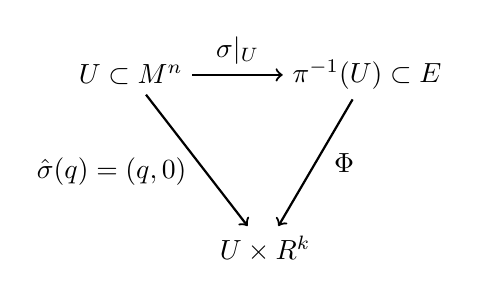
\begin{tikzpicture}[scale=0.7][node distance=3cm, auto, >=Stealth]
			% Nodos
			\node (U) {$U \subset M^n$};
			\node (E) [right of=U, xshift=2cm] {$\pi^{-1}(U) \subset E$};
			\node (R) [below right of=U, xshift=1cm, yshift=-1.5cm] {$U \times \mathbb{R}^k$};
			
			% Setas
			\draw[->, thick] (U) -- node[above] {$\sigma|_U$} (E);
			\draw[->, thick] (E) -- node[right, xshift=3pt] {$\Phi$} (R);
			\draw[->, thick] (U) -- node[left, swap, yshift=-4pt] {$\hat{\sigma}(q) = (q, 0)$} (R);
		\end{tikzpicture}
		\caption{Diagrama comutativo da representação local da seção zero $\sigma$ no fibrado trivializado.}
	\end{figure}
	
	\textbf{3. Conclusão da Suavidade Global da Seção Zero}
	
	Temos estabelecida a relação de composição $\Phi \circ \sigma|_U = \hat{\sigma}$. Uma vez que a trivialização local $\Phi$ é um difeomorfismo entre $\pi^{-1}(U)$ e $U \times \mathbb{R}^k$ (conforme a definição de fibrado vetorial no Capítulo 5 do Lee), ela possui uma inversa $\Phi^{-1} : U \times \mathbb{R}^k \to \pi^{-1}(U)$ que é estritamente suave. 
	
	Podemos então isolar a restrição da seção zero compondo ambos os lados à esquerda por esta inversa suave:
	\begin{equation*}
		\sigma|_U = \Phi^{-1} \circ \hat{\sigma}.
	\end{equation*}
	Pelo Teorema da Composição de Funções Suaves (Lee, Cap. 2), a composição de duas aplicações suaves ($\Phi^{-1}$ e $\hat{\sigma}$) resulta necessariamente em uma aplicação suave. Assim, demonstramos conclusivamente que $\sigma|_U$ é suave. 
	
	Visto que o ponto $p$ foi tomado arbitrariamente em $M^n$, a aplicação $\sigma$ é localmente suave na vizinhança de absolutamente todos os pontos de $M^n$. Logo, a seção zero $\sigma: M^n \to E$ é globalmente suave em todo o fibrado.
}

%%%% QUESTÃO 03 %%%%	
\questao{Seja $\pi:E\rightarrow M^{n}$ um fibrado vetorial suave de posto k. Mostre que todo referencial local suave $(\sigma_{1},...,\sigma_{k})$ para E em U é associado com alguma trivialização local $\Phi:\pi^{-1}(U)\rightarrow U\times\mathbb{R}^{k}$.
}
\solucao{
	
	\textbf{Análise do Enunciado}
	\begin{itemize}
		\item \textbf{Hipóteses:} $\pi: E \to M^n$ é um fibrado vetorial suave de posto $k$. Temos um conjunto aberto $U \subset M^n$ e uma coleção de $k$ seções locais suaves $\sigma_1, \dots, \sigma_k : U \to \pi^{-1}(U)$ que formam um referencial local. Isso significa que, para todo ponto $p \in U$, o conjunto de vetores $\{\sigma_1(p), \dots, \sigma_k(p)\}$ constitui uma base para a fibra vetorial $E_p = \pi^{-1}(p)$.
		\item \textbf{Tese:} Demonstrar a existência de uma trivialização local suave $\Phi: \pi^{-1}(U) \to U \times \mathbb{R}^k$ que corresponda a este referencial.
	\end{itemize}
	
	\textbf{Desenvolvimento Formal}
	
	A demonstração consiste em construir uma parametrização local $\Psi$ a partir do referencial dado, provar que ela é bijetora e suave e, em seguida, mostrar que a sua inversa $\Phi = \Psi^{-1}$ é a trivialização suave procurada.
	
	\textbf{1. Construção da Parametrização Trivializante $\Psi$}
	
	Definimos uma aplicação $\Psi: U \times \mathbb{R}^k \to \pi^{-1}(U)$. Para qualquer par $(p, v) \in U \times \mathbb{R}^k$, onde o vetor $v$ é dado por suas coordenadas $v = (v^1, \dots, v^k) \in \mathbb{R}^k$, definimos $\Psi$ utilizando a \textbf{Notação de Einstein}:
	\begin{equation*}
		\Psi(p, v) = v^i \sigma_i(p).
	\end{equation*}
	
	Para verificar a suavidade de $\Psi$, tomamos um ponto arbitrário $p_0 \in U$. Como $\pi: E \to M^n$ é um fibrado vetorial suave, existe por definição um aberto $W \subset U$ contendo $p_0$ e uma trivialização local suave $\Theta: \pi^{-1}(W) \to W \times \mathbb{R}^k$. Na trivialização $\Theta$, cada seção suave $\sigma_i$ restrita a $W$ é expressa como $\Theta(\sigma_i(p)) = (p, s_i(p))$, onde $s_i: W \to \mathbb{R}^k$ são aplicações suaves. 
	
	Avaliando $\Psi$ nesta trivialização local e usando a linearidade nas fibras:
	\begin{equation*}
		\Theta \circ \Psi(p, v) = \Theta( v^i \sigma_i(p) ) = ( p, v^i s_i(p) ).
	\end{equation*}
	Como as componentes $v^i$ são projeções suaves e as aplicações $s_i(p)$ são suaves, a combinação linear acima é suave em $W \times \mathbb{R}^k$. Logo, $\Psi$ é suave.
	
	\textbf{2. Bijectividade e Definição de $\Phi$}
	
	Para cada $p \in U$, a restrição $\Psi_p : \mathbb{R}^k \to E_p$ é dada por $\Psi_p(v) = v^i \sigma_i(p)$. Como $\{\sigma_i(p)\}$ é uma base de $E_p$, $\Psi_p$ é um isomorfismo linear. Assim, $\Psi$ é uma bijeção e definimos a trivialização como:
	\begin{equation*}
		\Phi = \Psi^{-1} : \pi^{-1}(U) \to U \times \mathbb{R}^k.
	\end{equation*}
	
	\textbf{3. Demonstração da Suavidade da Inversa $\Phi$}
	
	Para provar que $\Phi$ é suave, analisamos sua representação local em $W$. Definimos a matriz $A(p)$ cujas colunas são os vetores $s_1(p), \dots, s_k(p)$. A componente $j$ do vetor $v^i s_i(p)$ é escrita em notação de Einstein como $A^j_i(p) v^i$. Assim, a representação local de $\Phi$ é $(p, w) \mapsto (p, [A(p)]^{-1} w)$. Apresentamos agora duas formas de concluir a suavidade desta inversão:
	
	\textit{\textbf{Via I: Abordagem por Grupos de Lie (Elegância Estrutural)}}
	\solucaoalt{
		A suavidade de $\Phi$ é garantida pois a representação local da aplicação $\Psi$ em uma trivialização pré-existente $\Theta$ é dada por $\Theta \circ \Psi(p, v) = (p, A(p)v)$. Conforme demonstrado na \textbf{Questão 35 da Lista 01}, o conjunto $GL(k, \mathbb{R})$ das matrizes inversíveis é um \textbf{Grupo de Lie}. Como tal, a aplicação de inversão $\text{Inv}: GL(k, \mathbb{R}) \to GL(k, \mathbb{R})$, dada por $A \mapsto A^{-1}$, é comprovadamente suave. 
		
		Visto que as seções $\sigma_i$ são suaves, a aplicação $A: W \to GL(k, \mathbb{R})$ é suave. Portanto, a representação de $\Phi$ via $\Theta$, dada por $(p, w) \mapsto (p, A(p)^{-1}w)$, é a composição de aplicações suaves entre variedades. Esta estrutura assegura que a inversão matricial preserva a suavidade, tornando $\Phi$ um difeomorfismo local.
	}
		
	\textit{\textbf{Via II: Abordagem Analítica (Regra de Cramer)}}
	Pela Regra de Cramer, as entradas da matriz inversa são dadas por:
	\begin{equation*}
		(A^{-1})^j_i(p) = \frac{1}{\det(A(p))} \text{Adj}(A(p))^j_i.
	\end{equation*}
	O determinante e a matriz adjunta são polinômios nas entradas $A^a_b(p)$. Como as entradas são suaves e $\det(A(p)) \neq 0$, o quociente é suave. O produto $[A(p)]^{-1} w$ em notação de Einstein é $(A^{-1})^j_i(p) w^i$, que é uma soma de produtos de funções suaves, logo, suave.
	
	\textbf{4. Conclusão}
	
	Em ambas as abordagens, $\Phi: \pi^{-1}(U) \to U \times \mathbb{R}^k$ é um difeomorfismo suave que preserva as fibras e age como isomorfismo linear nelas. Portanto, $\Phi$ é a trivialização local associada ao referencial $(\sigma_i)$.
}

%%%% QUESTÃO 04 %%%%
\questao{Seja $M^n$ uma $n$-variedade suave. Então a estrutura suave já construída no fibrado tangente $TM$ é a única com respeito a qual $\pi : TM \to M^n$ é um fibrado vetorial suave de posto $n$ sobre $M^n$ e cujos campos vetoriais coordenados são seções locais suaves.}

\solucao{
	
	\textbf{Análise do Enunciado:}
	\begin{itemize}
		\item \textbf{Hipóteses:} $M^n$ é uma $n$-variedade suave; $TM$ é o seu fibrado tangente; $\pi: TM \to M^n$ é a projeção natural.
		\item \textbf{Tese:} A estrutura suave de fibrado vetorial em $TM$ é única sob a condição de que os campos coordenados $\tfrac{\partial}{\partial x^i}$ sejam seções locais suaves.
	\end{itemize}
	
	\textbf{Fundamentação Teórica}
	\begin{enumerate}
		\item \textbf{Referenciais e Trivializações (Questão 3, Lista 03):} Estabelecemos que qualquer referencial local suave $(\sigma_1, \dots, \sigma_k)$ em um fibrado vetorial induz univocamente uma trivialização local suave $\Phi: \pi^{-1}(U) \to U \times \mathbb{R}^k$.
		\item \textbf{Unicidade de Atlas (Questão 1, Lista 01):} A estrutura suave de uma variedade é univocamente determinada por seu atlas maximal. Dois atlas suavemente compatíveis definem a mesma estrutura.
	\end{enumerate}
	
	\textbf{Desenvolvimento Formal}
	
	Seja $\mathcal{E}$ qualquer estrutura de variedade suave em $TM$ que satisfaça as condições do enunciado. Consideremos uma carta coordenada $(U, (x^1, \dots, x^n))$ em $M^n$. 
	
	Por definição de espaço tangente, os campos vetoriais coordenados $\left\{ \tfrac{\partial}{\partial x^1}, \dots, \tfrac{\partial}{\partial x^n} \right\}$ formam uma base de $T_p M$ para todo $p \in U$. Pela hipótese do enunciado, esses campos são seções locais suaves sob a estrutura $\mathcal{E}$. Portanto, eles constituem, rigorosamente, um \textbf{referencial local suave} para o fibrado vetorial $(TM, \mathcal{E})$ sobre o aberto $U$.
	
	Aplicando o resultado da \textbf{Questão 3 desta Lista}, a existência deste referencial local suave implica a existência de uma única trivialização local suave $\Phi : \pi^{-1}(U) \to U \times \mathbb{R}^n$ associada a ele, tal que:
	\begin{equation*}
		\Phi\left( \sum_{i=1}^n v^i \tfrac{\partial}{\partial x^i} \right) = (p, (v^1, \dots, v^n)).
	\end{equation*}
	Esta aplicação $\Phi$ é precisamente a trivialização canônica utilizada na construção da estrutura suave padrão de $TM$ (conforme detalhado na Questão 13 da Lista 02 e reafirmado na Questão 1 desta Lista). 
	
	Sendo assim, para qualquer carta de $M^n$, a estrutura $\mathcal{E}$ deve admitir as mesmas trivializações locais que a estrutura canônica. Isso implica que o atlas de trivializações de $\mathcal{E}$ é suavemente compatível com o atlas canônico de $TM$, pois as funções de transição serão idênticas.
	
	Pela \textbf{Questão 1 da Lista 01}, dois atlas suavemente compatíveis pertencem ao mesmo atlas maximal. Portanto, a estrutura suave $\mathcal{E}$ deve coincidir com a estrutura suave canônica de $TM$. Esta prova demonstra a rigidez da estrutura do fibrado tangente: ela é inteiramente determinada pela suavidade dos campos coordenados da base.
}

%%%% QUESTÃO 05 %%%%
\questao{
	Seja $\pi : E \to M$ um fibrado vetorial suave de posto $k$ e suponha que $\sigma_{1}, \dots, \sigma_{m}$ sejam seções locais suaves independentes sobre um conjunto aberto $U \subset M$. Mostre que, para cada $p \in U$, existem seções suaves $\sigma_{m+1}, \dots, \sigma_{k}$ definidas em alguma vizinhança $V$ de $p$ tal que $(\sigma_{1}, \dots, \sigma_{k})$ é um referencial local suave para $E$ em $U \cap V$.
}
\solucao{
	
	\textbf{Análise do Enunciado}
	\begin{itemize}
		\item \textbf{Hipóteses:} $\pi: E \to M$ é um fibrado vetorial suave de posto $k$. As seções locais $\sigma_1, \dots, \sigma_m \in \Gamma(U, E)$ são linearmente independentes em cada fibra $E_q$ para todo $q \in U$.
		\item \textbf{Tese:} Para cada ponto $p \in U$, provar a existência de seções suaves $\sigma_{m+1}, \dots, \sigma_k$ em uma vizinhança $V \ni p$ tais que o conjunto total $\{\sigma_1, \dots, \sigma_k\}$ constitua um referencial local suave (base suave) para $E$ sobre $U \cap V$.
	\end{itemize}
	
	\textbf{Fundamentação Teórica}
	\begin{enumerate}
		\item \textbf{Completamento de Base (Álgebra Linear):} Dado que $E_p$ é um espaço vetorial de dimensão $k$, qualquer conjunto de $m < k$ vetores linearmente independentes pode ser estendido a uma base de $E_p$.
		\item \textbf{Estrutura de Fibrados (Lee, Cap. 5):} A existência de trivializações locais garante que podemos expressar qualquer seção suave como uma combinação linear de seções de um referencial local pré-existente com coeficientes suaves.
		\item \textbf{Estabilidade da Independência Linear:} A condição de que um conjunto de vetores seja linearmente independente é equivalente a a não-anulação do determinante de sua matriz de representação. Como o determinante é uma função contínua, a independência linear é uma propriedade aberta.
	\end{enumerate}
	
	\textbf{Desenvolvimento Formal}
	
	\textbf{1. Extensão Pontual em $p$}
	Seja $p \in U$. Por hipótese, o conjunto $\{\sigma_1(p), \dots, \sigma_m(p)\}$ é linearmente independente no espaço vetorial $E_p$. Pelo Teorema do Completamento de Base, existem vetores $v_{m+1}, \dots, v_k \in E_p$ tais que o conjunto $\{\sigma_1(p), \dots, \sigma_m(p), v_{m+1}, \dots, v_k\}$ seja uma base de $E_p$.
	
	\textbf{2. Construção de Seções Suaves Globais}
	Para propagar esses vetores $v_j$ para a vizinhança de $p$, utilizamos a estrutura de fibrado. Seja $(\tau_1, \dots, \tau_k)$ um referencial local suave definido em um aberto $W \ni p$. Cada vetor $v_j$ pode ser escrito univocamente como:
	\begin{equation*}
		v_j = \sum_{i=1}^k C_j^i \tau_i(p), \quad \text{com } C_j^i \in \mathbb{R}.
	\end{equation*}
	Definimos as seções $\sigma_j : W \to E$ para $j = m+1, \dots, k$ por:
	\begin{equation*}
		\sigma_j(q) = \sum_{i=1}^k C_j^i \tau_i(q), \quad \forall q \in W.
	\end{equation*}
	Visto que cada $\tau_i$ é uma seção suave e os $C_j^i$ são constantes, as seções $\sigma_j$ são, por definição, suaves em $W$. Note que, por construção, $\sigma_j(p) = v_j$.
	
	\textbf{3. Verificação da Independência Linear na Vizinhança}
	Seja $\mathcal{S}(q) = (\sigma_1(q), \dots, \sigma_k(q))$ o conjunto de seções em $U \cap W$. Para analisar a independência linear, expressamos cada $\sigma_\alpha$ em termos do referencial $\tau_\beta$:
	\begin{equation*}
		\sigma_\alpha(q) = A^\beta_\alpha(q) \tau_\beta(q), \quad \alpha, \beta \in \{1, \dots, k\}.
	\end{equation*}
	As funções $A^\beta_\alpha : U \cap W \to \mathbb{R}$ são as componentes coordenadas das seções $\sigma_\alpha$, logo são suaves. A matriz $[A^\beta_\alpha(q)]$ é a matriz de transição entre os referenciais. 
	
	No ponto $p$, o conjunto $\{\sigma_\alpha(p)\}$ é uma base de $E_p$, o que implica que $\det[A^\beta_\alpha(p)] \neq 0$. Sendo a função $\det[A^\beta_\alpha(\cdot)]$ contínua, existe uma vizinhança aberta $V \subset U \cap W$ de $p$ tal que $\det[A^\beta_\alpha(q)] \neq 0$ para todo $q \in V$. 
	
	Nesse aberto $V$, o determinante não nulo garante que as seções $\{\sigma_1(q), \dots, \sigma_k(q)\}$ permanecem linearmente independentes em cada fibra $E_q$. Como são $k$ vetores independentes em um espaço de dimensão $k$, eles formam um referencial local suave para $E$ em $V$.
}
\solucaoalt{
	\textbf{Demonstração via Topologia do Grupo de Lie $GL(k, \mathbb{R})$}
	
	A matriz de transição define uma aplicação suave $\mathcal{A}: U \cap W \to M(k, \mathbb{R})$ dada por $q \mapsto [A^\beta_\alpha(q)]$. O conjunto das matrizes inversíveis $GL(k, \mathbb{R})$ é um Grupo de Lie e, portanto, um subconjunto aberto de $M(k, \mathbb{R})$.
	
	Como $\{\sigma_\alpha(p)\}$ é base, temos $\mathcal{A}(p) \in GL(k, \mathbb{R})$. Pela continuidade de $\mathcal{A}$, a pré-imagem $\mathcal{A}^{-1}(GL(k, \mathbb{R}))$ é um aberto em $U \cap W$. Definindo $V$ como esse aberto, garantimos que $\mathcal{A}(q)$ é invertível para todo $q \in V$, o que assegura que as seções formam um referencial local suave.
}

%%% DEFINIÇÃO %%%
Antes de procedermos à resolução da Questão, convém notar que a análise de certos problemas geométricos pode ser significativamente enriquecida se abordada sob uma perspectiva estrutural. Para viabilizar as \textbf{soluções alternativas} que apresentaremos a seguir, e para evitar a redundância de definições algébricas no corpo das provas, estabelecemos previamente o seguinte resultado fundamental. Este servirá como o suporte teórico necessário para que a transição entre a álgebra e a geometria ocorra de forma natural e rigorosa.

%%%% RESULTADO EXTRA %%%%
\resultadoextra{Álgebra dos Quatérnios ($\mathbb{H}$)}{
	O corpo dos quatérnios $\mathbb{H}$ é uma álgebra de divisão sobre os reais com 4 dimensões. Um quatérnio $q \in \mathbb{H}$ é escrito como:
	\begin{equation*}
		q = a + b\mathbf{i} + c\mathbf{j} + d\mathbf{k}, \quad a, b, c, d \in \mathbb{R}
	\end{equation*}
	
	As unidades imaginárias $\mathbf{i}$, $\mathbf{j}$, $\mathbf{k}$ obedecem às regras fundamentais:
	\begin{equation*}
		\mathbf{i}^2 = \mathbf{j}^2 = \mathbf{k}^2 = \mathbf{i}\mathbf{j}\mathbf{k} = -1
	\end{equation*}
	Desta definição, derivam-se as relações de anticomutatividade: $\mathbf{ij} = \mathbf{k}, \mathbf{jk} = \mathbf{i}, \mathbf{ki} = \mathbf{j}$ e $\mathbf{ji} = -\mathbf{k}, \mathbf{kj} = -\mathbf{i}, \mathbf{ik} = -\mathbf{j}$.
	
	A norma de um quatérnio é definida por $|q|^2 = a^2 + b^2 + c^2 + d^2$. Uma propriedade fundamental é que a norma é multiplicativa: $|q \cdot p| = |q| \cdot |p|$ para quaisquer $q, p \in \mathbb{H}$.
	
	Consequentemente, o conjunto de quatérnios unitários $\mathbb{S}^3 = \{q \in \mathbb{H} : |q| = 1\}$ forma um grupo sob a multiplicação de quatérnios, sendo, portanto, um Grupo de Lie de dimensão 3.
}

%%%% QUESTÃO 06 %%%%
\questao{
	Considere os seguintes campos vetoriais em $\mathbb{R}^{4}$:
	$$X_{1}=-x^{2}t\frac{\partial}{\partial x^{1}}+x^{1}\tfrac{\partial}{\partial x^{2}}+x^{4}\tfrac{\partial}{\partial x^{3}}-x^{3}\tfrac{\partial}{\partial x^{4}}$$
	$$X_{2}=-x^{3}\tfrac{\partial}{\partial x^{1}}-x^{4}\tfrac{\partial}{\partial x^{2}}+x^{1}\tfrac{\partial}{\partial x^{3}}+x^{2}\tfrac{\partial}{\partial x^{4}}$$
	$$X_{3}=-x^{4}\tfrac{\partial}{\partial x^{1}}+x^{3}\tfrac{\partial}{\partial x^{2}}-x^{2}\tfrac{\partial}{\partial x^{3}}+x^{1}\tfrac{\partial}{\partial x^{4}}$$
	Mostre que existem campos vetoriais suaves $V_{1}, V_{2}, V_{3}$ em $\mathbb{S}^{3}$ tais que $V_{j}$ é $\iota$-relacionado a $X_{j}$ para $j=1,2,3,$ onde $\iota:\mathbb{S}^{3}\rightarrow\mathbb{R}^{4}$ é a aplicação inclusão.
	Conclua que $\mathbb{S}^{3}$ é paralelizável.
}
\solucao{
	
	\textbf{Análise do Enunciado}
	\begin{itemize}
		\item \textbf{Hipóteses:} $X_1, X_2, X_3 \in \mathfrak{X}(\mathbb{R}^4)$. $\mathbb{S}^3 \subset \mathbb{R}^4$ é a subvariedade mergulhada definida pela inclusão $\iota$.
		\item \textbf{Tese 1:} Provar que $X_j$ são tangentes a $\mathbb{S}^3$, garantindo a existência de $V_j \in \mathfrak{X}(\mathbb{S}^3)$.
		\item \textbf{Tese 2:} Provar que $\{V_1, V_2, V_3\}$ formam um referencial global suave para $\mathbb{S}^3$.
	\end{itemize}
	
	\textbf{Fundamentação Teórica}
	\begin{enumerate}
		\item \textbf{Tangencialidade:} Um campo $X \in \mathfrak{X}(\mathbb{R}^4)$ é tangente a $\mathbb{S}^3$ se, para todo $p \in \mathbb{S}^3$, $\langle X(p), p \rangle = 0$.
		\item \textbf{Paralelizabilidade:} $\mathbb{S}^3$ é paralelizável se admite 3 campos suaves globais que são linearmente independentes em cada ponto.
	\end{enumerate}
	
	\textbf{Desenvolvimento Formal}
	
	\textbf{1. Verificação da Tangencialidade}
	Seja $p = (x^1, x^2, x^3, x^4) \in \mathbb{S}^3$. O produto escalar entre $p$ e os campos $X_j$ é:
	\begin{align*}
		\langle X_1, p \rangle &= (-x^2)(x^1) + (x^1)(x^2) + (x^4)(x^3) + (-x^3)(x^4) = 0. \\
		\langle X_2, p \rangle &= (-x^3)(x^1) + (-x^4)(x^2) + (x^1)(x^3) + (x^2)(x^4) = 0. \\
		\langle X_3, p \rangle &= (-x^4)(x^1) + (x^3)(x^2) + (-x^2)(x^3) + (x^1)(x^4) = 0.
	\end{align*}
	Como $\langle X_j, p \rangle = 0$ para todo $j \in \{1, 2, 3\}$, os campos $X_j$ são tangentes a $\mathbb{S}^3$. Logo, existem campos $V_j \in \mathfrak{X}(\mathbb{S}^3)$ tais que $\iota_* V_j = X_j$.
	
	\textbf{2. Independência Linear Global}
	Calculamos a ortogonalidade dos campos no ambiente $\mathbb{R}^4$:
	\begin{align*}
		\langle X_1, X_2 \rangle &= (-x^2)(-x^3) + (x^1)(-x^4) + (x^4)(x^1) + (-x^3)(x^2) = 0. \\
		\langle X_1, X_3 \rangle &= (-x^2)(-x^4) + (x^1)(x^3) + (x^4)(-x^2) + (-x^3)(x^1) = 0. \\
		\langle X_2, X_3 \rangle &= (-x^3)(-x^4) + (-x^4)(x^3) + (x^1)(-x^2) + (x^2)(x^1) = 0.
	\end{align*}
	As normas são $\|X_1\|^2 = \|X_2\|^2 = \|X_3\|^2 = \sum (x^i)^2 = 1$ para $p \in \mathbb{S}^3$.
	
	Visto que $\{V_1(p), V_2(p), V_3(p)\}$ formam um conjunto ortonormal em $T_p\mathbb{S}^3$ para todo $p$, eles são linearmente independentes. Como $\dim(\mathbb{S}^3) = 3$, eles constituem um referencial global suave. Portanto, $\mathbb{S}^3$ é paralelizável.
}

\solucaoalt{
	\textbf{Abordagem via Estrutura de Grupo de Lie ($\mathbb{H}$)}
	
	Utilizando a estrutura de Quatérnios definida no \textbf{Resultado Extra anterior}, identificamos $\mathbb{S}^3$ como o Grupo de Lie dos quatérnios unitários.
	
	Os campos $X_j$ são gerados pela translação à direita de $x \in \mathbb{S}^3$ pelas unidades imaginárias $\{\mathbf{i}, \mathbf{j}, \mathbf{k}\}$ da base de $\mathbb{H}$:
	\begin{align*}
		X_1(x) &= x \cdot \mathbf{i} = (-x^2, x^1, x^4, -x^3) \\
		X_2(x) &= x \cdot \mathbf{j} = (-x^3, -x^4, x^1, x^2) \\
		X_3(x) &= x \cdot \mathbf{k} = (-x^4, x^3, -x^2, x^1)
	\end{align*}
	Sendo a multiplicação de quatérnios uma operação suave, os campos $X_j$ são suaves. Como a multiplicação por unidades imaginárias preserva a norma ($|x \cdot \mathbf{i}| = |x| \cdot 1 = 1$), os vetores $X_j(x)$ são tangentes a $\mathbb{S}^3$ (pois a derivada de $\|x\|^2=1$ em qualquer direção de translação de grupo é nula).
	
	Como $\{\mathbf{i}, \mathbf{j}, \mathbf{k}\}$ é uma base para o espaço tangente à identidade $T_1\mathbb{S}^3$, e a translação à direita em um Grupo de Lie é um difeomorfismo que preserva a independência linear, os campos $\{V_1, V_2, V_3\}$ formam obrigatoriamente um referencial global suave para $T\mathbb{S}^3$. Assim, a paralelizabilidade de $\mathbb{S}^3$ decorre da sua estrutura de Grupo de Lie.
}

%%%% QUESTÃO 07 %%%%
\questao{Seja $M^{n}$ uma n-variedade suave e $T^{*}M$ seu fibrado cotangente. Com sua projeção natural e com a estrutura vetorial de cada fibra, mostre que TM é o único fibrado vetorial suave de posto n sobre $M^{n}$ para o qual todos os campos de covetores coordenados são seções locais suaves.}

\solucao{
	
	\textbf{Análise do Enunciado}
	\begin{itemize}
		\item \textbf{Hipóteses:} $M^n$ é uma variedade suave. O conjunto $T^*M = \coprod_{p \in M} T_p^*M$ é o fibrado cotangente munido de sua projeção natural $\pi: T^*M \to M^n$. (Nota analítica: o enunciado original grafa "TM" na segunda proposição, mas o contexto de "campos de covetores coordenados" e a premissa inicial definem inequivocamente que a tese se refere ao espaço total $T^*M$).
		\item \textbf{Tese:} Provar que a estrutura suave padrão de $T^*M$ é a única estrutura de variedade que torna $\pi$ um fibrado vetorial suave sob a condição de que, para qualquer carta, os diferenciais coordenados $(dx^1, \dots, dx^n)$ atuem como seções locais suaves.
	\end{itemize}
	
	\textbf{Fundamentação Teórica}
	\begin{enumerate}
		\item \textbf{Atlas do Fibrado Cotangente:} A estrutura suave padrão de $T^*M$ é fundamentada nas cartas naturais $(T^*U, \tilde{\phi})$. Para uma carta $(U, \phi)$ de $M^n$ com coordenadas $(x^1, \dots, x^n)$, um covetor $\omega_p \in T_p^*M$ escreve-se, em notação de Einstein, como $\omega_p = \omega_i dx^i|_p$. A carta natural é dada por $\tilde{\phi}(\omega_p) = (x^1(p), \dots, x^n(p), \omega_1, \dots, \omega_n)$.
		\item \textbf{Referenciais e Trivializações (Questão 3):} Todo referencial local suave determina univocamente uma trivialização local suave para o fibrado.
		\item \textbf{Atlas Maximal (Questão 1 da Lista 01):} Atlas suavemente compatíveis definem uma única estrutura suave.
	\end{enumerate}
	
	\textbf{Desenvolvimento Formal}
	
	Suponha que exista uma estrutura de variedade suave $\mathcal{E}$ no conjunto $T^*M$ com respeito à qual $\pi: T^*M \to M^n$ seja um fibrado vetorial suave e tal que, para qualquer carta suave $(U, (x^1, \dots, x^n))$ da variedade base $M^n$, os campos de covetores coordenados $(dx^1, \dots, dx^n)$ sejam seções locais estritamente suaves.
	
	Para cada ponto $p \in U$, os covetores $dx^1|_p, \dots, dx^n|_p$ formam a base dual do espaço cotangente $T_p^*M$. Como assumimos por hipótese que estas seções são suaves na estrutura $\mathcal{E}$, a coleção ordenada $(dx^1, \dots, dx^n)$ constitui um referencial local suave para $T^*M$ sobre o aberto $U$.
	
	Pela equivalência demonstrada rigorosamente na \textbf{Questão 3}, este referencial local suave induz uma única trivialização local suave na estrutura $\mathcal{E}$. Denotemos esta trivialização por $\Phi: \pi^{-1}(U) \to U \times \mathbb{R}^n$. Atuando sobre um covetor genérico $\omega_p = \omega_i dx^i|_p$, a trivialização extrai as coordenadas:
	\begin{equation*}
		\Phi(\omega_i dx^i|_p) = (p, (\omega_1, \dots, \omega_n)).
	\end{equation*}
	
	Sendo $\mathcal{E}$ uma estrutura de fibrado vetorial, $\Phi$ é um difeomorfismo local em relação a $\mathcal{E}$.
	
	Analisemos a relação desta trivialização $\Phi$ com a carta padrão $\tilde{\phi}$ do fibrado cotangente. A aplicação de transição é dada por:
	\begin{equation*}
		\tilde{\phi} \circ \Phi^{-1}(p, (\omega_1, \dots, \omega_n)) = \tilde{\phi}(\omega_i dx^i|_p) = (\phi(p), \omega_1, \dots, \omega_n).
	\end{equation*}
	Esta composição é essencialmente o produto direto $\phi \times \text{Id}_{\mathbb{R}^n}$. Sendo $\phi: U \to \mathbb{R}^n$ um difeomorfismo suave da variedade base, a aplicação produto preserva o difeomorfismo.
	
	Logo, as cartas geradas pelas trivializações na estrutura $\mathcal{E}$ são suavemente compatíveis com as cartas naturais que definem a estrutura padrão de $T^*M$. Conclui-se, pelo Lema do Atlas Maximal, que as estruturas são idênticas. A estrutura suave padrão é, portanto, única.
}
\solucaoalt{
	
	\textbf{Demonstração via Transições no Grupo de Lie $GL(n, \mathbb{R})$}
	
	A unicidade da estrutura do fibrado pode ser atestada analisando o comportamento das funções de transição no Grupo de Lie associado ao fibrado.
	
	Sejam $(U, (x^i))$ e $(V, (y^j))$ duas cartas coordenadas suaves superpostas em $M^n$. Na interseção $U \cap V$, a mudança de base no espaço cotangente é regida pela matriz Jacobiana transposta inversa. Em notação de Einstein, a transição entre os referenciais é:
	\begin{equation*}
		dy^j = \tfrac{\partial y^j}{\partial x^i} dx^i.
	\end{equation*}
	A matriz de transição $\mathcal{A}(p)$ cujas entradas são $A^j_i(p) = \tfrac{\partial y^j}{\partial x^i}(p)$ é, em cada ponto, não-singular. Portanto, a aplicação $p \mapsto \mathcal{A}(p)$ mapeia pontos da variedade no Grupo de Lie $GL(n, \mathbb{R})$.
	
	Como as cartas da base são difeomorfismos, as derivadas parciais $\tfrac{\partial y^j}{\partial x^i}$ são funções de classe $C^\infty$. Assim, a aplicação de transição para $GL(n, \mathbb{R})$ é estritamente suave.
	
	Qualquer estrutura de fibrado vetorial $\mathcal{E}$ em $T^*M$ que torne as seções coordenadas $(dx^i)$ suaves será obrigatoriamente \textbf{colada} pelas mesmas funções de transição suaves avaliadas em $GL(n, \mathbb{R})$. Como provamos na \textbf{Questão 1}, a identidade dessas funções de transição dita uma única estrutura de fibrado vetorial suave. Portanto, a estrutura $\mathcal{E}$ coincide topológica e algebricamente com a estrutura padrão.
}

%%%% QUESTÃO 08 %%%%
\questao{Sejam $M^{n}$ uma $n$-variedade suave e $\omega:M^{n}\rightarrow T^{*}M$ uma seção áspera.
	\begin{enumerate}[label=(\alph*)]
		\item Se $\omega=\sum_{i=1}^{n}\omega_{i}dx^{i}$ é a representação coordenada para $\omega$ em uma carta coordenada suave arbitrária $(U,(x^{i}))$, então mostre que $\omega$ é suave em $U$ se, e somente se, suas funções componentes são suaves.
		\item Mostre que $\omega$ é suave se, e somente se, para qualquer campo de vetores suave $X$ sobre um conjunto aberto $U\subset M^{n}$, a função $\omega(X): U \to \mathbb{R}$, definida por $\omega(X)(p)=\omega_{p}(X_{p})$ para todo $p\in U$, é suave.
	\end{enumerate}
}
\solucao{
	
	\textbf{Análise Detalhada do Enunciado}
	\begin{itemize}
		\item \textbf{Configuração Geométrica:} $M^n$ é uma variedade suave e $T^*M$ é o seu fibrado cotangente. Uma seção áspera $\omega$ associa a cada ponto $p \in M$ um covetor $\omega_p \in T_p^*M$, sem assumir a priori a suavidade da aplicação $\omega: M \to T^*M$.
		\item \textbf{Objetivo:} Estabelecer a equivalência entre a suavidade da seção (como mapa entre variedades) e a suavidade de suas componentes locais (a) e a suavidade de sua contração com campos vetoriais (b).
	\end{itemize}
	
	\textbf{Fundamentação Teórica}
	\begin{enumerate}
		\item \textbf{Trivializações do Fibrado Cotangente:} A estrutura suave de $T^*M$ é definida por cartas $\tilde{\phi}$ que mapeia $\omega_p = \omega_i dx^i|_p$ para $(x(p), \omega_1, \dots, \omega_n)$. Uma seção é suave se sua representação local $\hat{\omega} = \tilde{\phi} \circ \omega$ for suave (Lee, Cap. 5).
		\item \textbf{Referenciais Suaves (Questão 3, Lista 03):} a coleção $\{dx^i\}$ constitui um referencial local suave para $T^*M$. Qualquer seção $\omega$ pode ser escrita como combinação linear deste referencial.
		\item \textbf{Dualidade e Contrações:} A função $\omega(X)$ é a avaliação do covetor $\omega_p$ no vetor $X_p$, denotada pelo pareamento dual $\langle \omega_p, X_p \rangle$.
	\end{enumerate}
	
	\textbf{Desenvolvimento Formal - Parte (a)}
	
	Seja $(U, (x^i))$ uma carta coordenada suave. A trivialização canônica $\Phi: T^*U \to \varphi(U) \times \mathbb{R}^n$ associa a cada covetor $\xi_p = \xi_i dx^i|_p$ o par $(\phi(p), (\xi_1, \dots, \xi_n))$.
	
	A seção $\omega$ é suave se, e somente se, a aplicação $\hat{\omega} = \Phi \circ \omega : U \to \varphi(U) \times \mathbb{R}^n$ for suave. A representação de $\hat{\omega}$ é:
	\begin{equation*}
		\hat{\omega}(p) = (\phi(p), \omega_1(p), \dots, \omega_n(p)).
	\end{equation*}
	As primeiras $n$ componentes são as coordenadas da própria variedade $M$, que são suaves por definição. Portanto, a suavidade de $\hat{\omega}$ depende exclusivamente da suavidade das funções componentes $\omega_i : U \to \mathbb{R}$. Assim, $\omega$ é suave em $U$ se, e somente se, cada $\omega_i$ é de classe $C^\infty$.
	
	\textbf{Desenvolvimento Formal - Parte (b)}
	
	\textbf{Condição Necessária ($\implies$):} Assumimos que $\omega$ é uma seção suave. Seja $X$ um campo de vetores suave em $U$, expresso na base coordenada como $X = X^j \tfrac{\partial}{\partial x^j}$. A função $\omega(X): U \to \mathbb{R}$ é definida pela avaliação do covetor $\omega_p$ sobre o vetor $X_p$ para cada $p \in U$:
	
	\begin{equation*}
		\omega(X)(p) = \omega_p(X_p) = \left( \omega_i(p) dx^i|_p \right) \left( X^j(p) \tfrac{\partial}{\partial x^j} \Big|_p \right) = \omega_i(p) X^j(p) \delta^i_j = \omega_i(p) X^i(p),
	\end{equation*}
	
	onde utilizamos a convenção de soma de Einstein e o fato de que $\{dx^i\}$ e $\left\{\tfrac{\partial}{\partial x^j}\right\}$ são bases duais, satisfazendo $dx^i \left( \tfrac{\partial}{\partial x^j} \right) = \delta^i_j$. Como as funções componentes $\omega_i$ e $X^i$ são suaves em $U$, o produto $\omega_i X^i$ também é uma função suave, provando que $\omega(X)$ é suave.
	
	\textbf{Condição Suficiente ($\impliedby$):} Assumimos que, para qualquer campo de vetores suave $X$ em $U$, a função $\omega(X): U \to \mathbb{R}$ é suave. Para extrair a suavidade das funções componentes $\omega_j$, consideramos os campos de vetores coordenados $\tfrac{\partial}{\partial x^j}$ para cada $j \in \{1, \dots, n\}$. Como estes são campos suaves por construção, a hipótese garante que a função $\omega\left(\tfrac{\partial}{\partial x^j}\right)$ é suave em $U$. Calculando a sua representação em cada ponto $p \in U$, temos:
	
	\begin{equation*}
		\omega\left(\tfrac{\partial}{\partial x^j}\right)(p) = \omega_p \left( \left. \tfrac{\partial}{\partial x^j} \right|_p \right) = \left( \omega_i(p) dx^i|_p \right) \left( \left. \tfrac{\partial}{\partial x^j} \right|_p \right) = \omega_i(p) \delta^i_j = \omega_j(p).
	\end{equation*}
	
	Como $\omega\left(\tfrac{\partial}{\partial x^j}\right)$ é uma função suave, conclui-se que cada função componente $\omega_j$ é suave em $U$. Pela fundamentação estabelecida na \textbf{Parte (a)}, a suavidade de todas as funções componentes $\omega_j$ é a condição necessária e suficiente para que a seção $\omega$ seja suave.
}
\solucaoalt{
	\textbf{Justificativa Estrutural via Dualidade de Fibrados}
	
	A suavidade de $\omega$ pode ser interpretada como uma propriedade da estrutura de fibrados. Como $M$ é suave, o fibrado tangente $TM$ possui funções de transição suaves (Jacobianas). O fibrado $T^*M$ é o dual de $TM$, e suas funções de transição são as transpostas das inversas das Jacobianas de $M$.
	
	A equivalência $\omega \text{ suave} \iff \omega(X) \text{ suave}$ reflete o fato de que a dualidade entre $TM$ e $T^*M$ é um isomorfismo suave de feixes. Em termos concretos, a avaliação de uma seção do fibrado dual em seções do fibrado original recupera a topologia da variedade base, permitindo a caracterização da suavidade de $\omega$ através da sua ação em campos vetoriais.
}

%%%% QUESTÃO 09 %%%%
\questao{Se $M^{n}$ é uma $n$-variedade suave, mostre que $T^*M$ é trivial se, e somente se, $TM$ é trivial.}
\solucao{
	
	\textbf{Análise do Enunciado}
	\begin{itemize}
		\item \textbf{Hipóteses:} $M^n$ é uma variedade suave. $TM$ é o fibrado tangente e $T^*M$ é o seu fibrado dual (cotangente).
		\item \textbf{Tese:} Provar a equivalência $\text{Trivialidade}(TM) \iff \text{Trivialidade}(T^*M)$.
	\end{itemize}
	
	\textbf{Fundamentação Teórica}
	\begin{enumerate}
		\item \textbf{Trivialidade de Fibrados (Lee, Cap. 5):} Um fibrado vetorial de posto $n$ é trivial se, e somente se, admite um referencial global suave, isto é, um conjunto de $n$ seções suaves $\{\sigma_1, \dots, \sigma_n\}$ que formam uma base de cada fibra em todo o domínio.
		\item \textbf{Base Dual (Álgebra Linear):} Para qualquer base $\{X_i\}$ de um espaço vetorial $V$, existe uma única base dual $\{\omega^j\}$ de $V^*$ tal que $\omega^j(X_i) = \delta^j_i$.
		\item \textbf{Reflexividade:} Para espaços vetoriais de dimensão finita, existe um isomorfismo canônico $\Psi : V \to V^{**}$.
	\end{enumerate}
	
	\textbf{Desenvolvimento Formal}
	
	\textit{Ida ($\impliedby$):} Assuma que $TM$ é trivial. Então, existe um referencial global suave $\{X_1, \dots, X_n\}$ para $TM$. Para cada $p \in M$, definimos a base dual $\{\omega^1(p), \dots, \omega^n(p)\}$ em $T_p^*M$ tal que $\omega^j(p)(X_i(p)) = \delta^j_i$.
	
	Para provar que cada $\omega^j$ é uma seção suave de $T^*M$, tomemos um campo vetorial suave qualquer $Y \in \mathfrak{X}(M)$. Podemos escrever $Y$ na base $\{X_i\}$ como $Y = \sum_{k=1}^n Y^k X_k$, onde as funções $Y^k: M \to \mathbb{R}$ são suaves, pois $X_i$ formam um referencial suave. A ação de $\omega^j$ sobre $Y$ é:
	\begin{equation*}
		\omega^j(Y) = \omega^j(\sum_{k=1}^n Y^k X_k) = \sum_{k=1}^n Y^k \omega^j(X_k) = \sum_{k=1}^n Y^k \delta^j_k = Y^j.
	\end{equation*}
	Visto que $\omega^j(Y) = Y^j$ e $Y^j$ é uma função suave para qualquer $Y \in \mathfrak{X}(M)$, segue da caracterização de suavidade de seções do fibrado cotangente (\textbf{Questão 8b da Lista 03}) que $\omega^j$ é uma seção suave. Logo, $\{\omega^j\}$ é um referencial global suave para $T^*M$, tornando-o trivial.
	
	\textit{Volta ($\implies$):} Assuma que $T^*M$ é trivial com referencial global suave $\{\theta^1, \dots, \theta^n\}$. Pela reflexividade de espaços de dimensão finita, cada $\theta^i(p) \in T_p^*M$ pode ser vista como um elemento de $(T_p^*M)^* \cong T_p M$.
	
	Definimos os campos vetoriais $V_j$ tais que $\theta^i(V_j) = \delta^i_j$. De forma análoga à prova anterior, para qualquer 1-forma suave $\omega = \sum \omega_k \theta^k$, temos que a contração $\omega(V_j) = \omega_j$. Como as componentes $\omega_j$ são suaves por hipótese de suavidade de $\omega$, a aplicação $p \mapsto V_j(p)$ é uma seção suave de $TM$. Assim, $\{V_j\}$ é um referencial global suave para $TM$, tornando-o trivial.
}
\solucaoalt{
	\textbf{Demonstração via Funções de Transição e Grupos de Lie}
	
	Um fibrado vetorial é trivial se, e somente se, suas funções de transição podem ser reduzidas à identidade $I \in GL(n, \mathbb{R})$ através de uma mudança de referencial.
	
	Sejam $\tau_{\alpha\beta}: U_\alpha \cap U_\beta \to GL(n, \mathbb{R})$ as funções de transição de $TM$. As funções de transição $\tilde{\tau}_{\alpha\beta}$ de $T^*M$ são dadas pela transposta da inversa:
	\begin{equation*}
		\tilde{\tau}_{\alpha\beta}(p) = (\tau_{\alpha\beta}(p)^{-1})^T.
	\end{equation*}
	Se $TM$ é trivial, existe um atlas cujas transições são $\tau_{\alpha\beta} = I$. Substituindo na fórmula acima:
	\begin{equation*}
		\tilde{\tau}_{\alpha\beta} = (I^{-1})^T = I^T = I.
	\end{equation*}
	A identidade das matrizes de transição implica que $T^*M$ também é trivial. Como a operação de inversão e transposição em $GL(n, \mathbb{R})$ é um difeomorfismo (Questão 35, Lista 01), a trivialidade de um fibrado implica a do seu dual.
}

%%%% QUESTÃO 10 %%%%
\questao{
	Considere $f : \mathbb{R}^3 \to \mathbb{R}$, $f(x,y,z) = x^2 + y^2 + z^2$ e a aplicação $F : \mathbb{R}^2 \to \mathbb{R}^3$ (inversa da projeção estereográfica). Calcule $F^* df$ e $d(f \circ F)$ separadamente, e verifique que são iguais.
}
\solucao{
	
	\textbf{Análise do Enunciado}
	\begin{itemize}
		\item \textbf{Hipóteses:} $f$ é uma função suave em $\mathbb{R}^3$ definida por $f(x,y,z) = x^2 + y^2 + z^2$. $F$ é a aplicação inversa da projeção estereográfica, que mapeia o plano $\mathbb{R}^2$ na esfera unitária $\mathbb{S}^2 \subset \mathbb{R}^3$.
		\item \textbf{Tese:} Calcular analiticamente a diferencial da composição $d(f \circ F)$ e o pullback $F^* df$, demonstrando a igualdade entre ambos.
	\end{itemize}
	
	\textbf{Fundamentação Teórica}
	Conforme a teoria de variedades suaves (Lee, Cap. 3 e 8), utilizamos:
	\begin{enumerate}
		\item \textbf{Diferencial de uma função (Lista 02):} Para $f \in C^\infty(M)$, a diferencial $df$ é a 1-forma única que, em cada ponto $p \in M$, atua sobre um vetor tangente $X \in T_p M$ como a derivação de $f$ na direção de $X$, isto é, $df_p(X) = X(f)$.
		\item \textbf{Pullback de diferenciais:} Seja $F : M \to N$ uma aplicação suave. O pullback $F^* df$ é definido tal que, para qualquer vetor $X \in T_p M$, temos $(F^* df)_p(X) = df_{F(p)}(dF_p X)$.
		\item \textbf{Diferencial como Derivação (Lista 02):} A ação da diferencial de $F$ no ponto $p$, $dF_p X$, sobre uma função $f$ é dada por $(dF_p X)(f) = X(f \circ F)$.
		\item \textbf{Inversa da Aplicação $F$ (Questão 3, Lista 01):} A inversa da projeção estereográfica é dada por:
		\begin{equation*}
			F(u, v) = \left( \frac{2u}{u^2+v^2+1}, \frac{2v}{u^2+v^2+1}, \frac{u^2+v^2-1}{u^2+v^2+1} \right).
		\end{equation*}
	\end{enumerate}
	\textbf{Desenvolvimento Formal:}
	
	Primeiro, calculamos a função composta $f \circ F$. Definindo $S = u^2 + v^2 + 1$, temos:
	\begin{align*}
		(f \circ F)(u,v) &=\left( \tfrac{2u}{S} \right)^2 + \left( \tfrac{2v}{S} \right)^2 + \left( \tfrac{u^2+v^2-1 \color{red}{+1-1}}{S} \right)^2 = \left( \tfrac{2u}{S} \right)^2 + \left( \tfrac{2v}{S} \right)^2 + \left( \tfrac{S-2}{S} \right)^2 \\
		& = \tfrac{4(u^2+v^2) + S^2 - 4S + 4}{S^2} = \tfrac{4(S-1) + S^2 - 4S + 4}{S^2} = \tfrac{S^2}{S^2} \\ 
		& = 1.
	\end{align*}
	Como a composta é a função constante $1$, sua diferencial é $d(f \circ F) = 0$.
	
	Para provar que $F^* df = 0$, tomamos um vetor tangente qualquer $X \in T_p \mathbb{R}^2$. Utilizando as definições de pullback e push-forward (estudadas na \textbf{Lista 02}), temos:
	\begin{align*}
		(F^* df)_p(X) = df_{F(p)}(dF_p X) = (dF_p X)(f) = X(f \circ F) = X(1) = 0.
	\end{align*}
	Como a igualdade $(F^* df)_p(X) = 0$ vale para qualquer ponto $p$ e qualquer vetor $X$, concluímos que $F^* df = 0$. Portanto, $F^* df = d(f \circ F)$.
}

%%%% RESULTADO EXTRA %%%%
\resultadoextra{Propriedades da Diferencial e Funções com Diferencial Nula}{
	
	\textbf{Proposição 6.9 (Propriedades da Diferencial).} Sejam $f, g \in C^\infty(M)$. Para provar as identidades abaixo, tomamos um ponto $p \in M$ e um vetor tangente $X \in T_p M$ qualquer. Utilizaremos a definição de diferencial: $df_p(X) = X(f)$.
	
	\begin{enumerate}[label=(\alph*)]
		\item \textbf{Linearidade:} $d(af + bg) = a \, df + b \, dg$.
		\begin{align*}
			(d(af + bg))_p(X) &= X(af + bg) \\
			&= a X(f) + b X(g) \quad \text{(pela linearidade de $X$ como derivação)} \\
			&= a \, df_p(X) + b \, dg_p(X) = (a \, df + b \, dg)_p(X).
		\end{align*}
		
		\item \textbf{Regra do Produto (Leibniz):} $d(fg) = f \, dg + g \, df$.
		\begin{align*}
			(d(fg))_p(X) &= X(fg) \\
			&= f(p) X(g) + g(p) X(f) \quad \text{(pela regra do produto para derivações)} \\
			&= f(p) dg_p(X) + g(p) df_p(X) = (f \, dg + g \, df)_p(X).
		\end{align*}
		
		\item \textbf{Regra do Quociente:} $d(f/g) = (g \, df - f \, dg)/g^2$ onde $g \neq 0$.
		\begin{align*}
			(d(f/g))_p(X) &= X(f/g) \\
			&= \frac{g(p) X(f) - f(p) X(g)}{(g(p))^2} \quad \text{(pela regra do quociente para derivações)} \\
			&= \frac{g(p) df_p(X) - f(p) dg_p(X)}{(g(p))^2} = \left( \frac{g \, df - f \, dg}{g^2} \right)_p(X).
		\end{align*}
		
		\item \textbf{Regra da Cadeia:} $d(h \circ f) = (h' \circ f) \, df$.
		\begin{align*}
			(d(h \circ f))_p(X) &= X(h \circ f) \\
			&= h'(f(p)) X(f) \quad \text{(pela regra da cadeia para derivações)} \\
			&= (h' \circ f)(p) \, df_p(X) = ((h' \circ f) \, df)_p(X).
		\end{align*}
		
		\item \textbf{Função Constante:} Se $f$ é constante, então $df = 0$.
		
		Como $f$ é constante, para qualquer curva $\gamma$ tal que $\gamma(0)=p$ e $\gamma'(0)=X$, a função $(f \circ \gamma)(t)$ é constante. Logo, $X(f) = \tfrac{d}{dt}(f \circ \gamma)(t) \big|_{t=0} = 0$. Assim, $df_p(X) = 0$ para todo $X$, logo $df = 0$.
	\end{enumerate}
	\textbf{Proposição 6.10 (Funções com Diferenciais Nulas).} Se $f$ é uma função suave em $M$, então $df = 0$ se, e somente se, $f$ é constante em cada componente conexa de $M$.
	
	\textbf{Prova:}
	
	$(\impliedby)$ Se $f$ é constante em uma componente conexa, então pela Proposição 6.9(e), $df = 0$ nessa componente. Como a diferencial é definida pontualmente, se $f$ é constante em todas as componentes, $df = 0$ em todo $M$.
	
	$(\implies)$ Suponha que $df = 0$. Seja $C$ uma componente conexa de $M$. Queremos mostrar que $f$ é constante em $C$. 
	Sejam $p, q \in C$. Como as componentes conexas de uma variedade suave são conexas por caminhos (\textbf{Questão 02 da Lista 01}), existe uma curva suave $\gamma : [0,1] \to C$ tal que $\gamma(0)=p$ e $\gamma(1)=q$.
	
	Considere a função real $h(t) = f(\gamma(t))$. Pela regra da cadeia (Proposição 6.9(d)), temos que	$\tfrac{dh}{dt} = df_{\gamma(t)}(\gamma'(t))$.
	
	Como, por hipótese, $df = 0$, temos $\tfrac{dh}{dt} = 0$ para todo $t \in [0,1]$. Do cálculo elementar, sabemos que uma função com derivada nula em um intervalo é constante. Logo, $h(0) = h(1)$, ou seja, $f(p) = f(q)$. Como $p$ e $q$ foram escolhidos arbitrariamente em $C$, $f$ é constante em $C$.\hfill\cqd
	
	\vspace{0.3cm}
	\textbf{\underline{Observação}:} Vale ressaltar que qualquer variedade suave $M$ pode ser decomposta como a união disjunta de suas componentes conexas, $M = \sqcup_{i \in I} C_i$. Como $M$ é localmente conexa, cada componente $C_i$ é, simultaneamente, um subconjunto aberto e fechado de $M$, herdando a estrutura de variedade suave. Portanto, a conclusão de que $f$ é constante em cada componente conexa $C_i$ estende a validade do resultado para a totalidade de $M$.
}


%%%% QUESTÃO 11 %%%%
\questao{Sejam $[a, b] \subset \mathbb{R}$ e $\omega$ um campo de covetores suave em $[a, b]$. Se $t$ denota a coordenada padrão em $[a, b]$, então $\omega = f(t)dt$ para alguma função suave $f : [a, b] \to \mathbb{R}$. Definimos a integral de $\omega$ em $[a, b]$ por $\int_{[a,b]} \omega = \int_a^b f(t)dt$. Mostre que:
	\begin{enumerate}[label=(\alph*)]
		\item Se $\varphi : [c, d] \to [a, b]$ é um difeomorfismo crescente, então $\int_{[c,d]} \varphi^* \omega = \int_{[a,b]} \omega$.
		\item Se $\varphi : [c, d] \to [a, b]$ é um difeomorfismo decrescente, então $\int_{[c,d]} \varphi^* \omega = -\int_{[a,b]} \omega$.
\end{enumerate}}

\solucao{
	
	\textbf{Análise do Enunciado:}
	\begin{itemize}
		\item \textbf{Hipóteses:} $\omega = f(t)dt$ é um campo de covetores suave em $[a,b]$. $\varphi : [c,d] \to [a,b]$ é um difeomorfismo (aplicação suave, bijetiva, com inversa suave). 
		\item \textbf{Tese:} Provar que a integral do pullback $\varphi^* \omega$ sobre $[c,d]$ coincide com a integral de $\omega$ sobre $[a,b]$ se $\varphi$ for crescente, e é a negativa desta se $\varphi$ for decrescente.
	\end{itemize}
	
	\textbf{Fundamentação Teórica:}
	\begin{enumerate}
		\item \textbf{Pullback de campos de covetores (Lee, Cap. 6):} Se $\omega = f dt$ é um campo de covetores em $\mathbb{R}$ e $\varphi : M \to \mathbb{R}$ é uma aplicação suave, o pullback é dado por $\varphi^* \omega = (f \circ \varphi) d\varphi$. Em coordenadas locais $t$ para $[c,d]$, temos $d\varphi = \tfrac{d\varphi}{dt} dt$.
		\item \textbf{Teorema de Mudança de Variável (Cálculo):} Para funções integráveis, $\int_{\varphi(c)}^{\varphi(d)} f(u) du = \int_c^d f(\varphi(t)) \varphi'(t) dt$.
	\end{enumerate}
	
	\textbf{Desenvolvimento Formal:}
	
	Primeiramente, determinamos a expressão do pullback $\varphi^* \omega$. Como $\omega = f(t)dt$, temos:
	\begin{equation*}
		\varphi^* \omega = \varphi^*(f(t)dt) = (f \circ \varphi)(t) d(\varphi(t)) = f(\varphi(t)) \varphi'(t) dt.
	\end{equation*}
	A integral de $\varphi^* \omega$ sobre o intervalo $[c,d]$ é, por definição:
	\begin{equation*}
		\int_{[c,d]} \varphi^* \omega = \int_c^d f(\varphi(t)) \varphi'(t) dt.
	\end{equation*}
	
	\textit{Análise do caso (a): $\varphi$ é um difeomorfismo crescente.}
	Como $\varphi$ é crescente e bijetiva de $[c,d]$ para $[a,b]$, temos obrigatoriamente $\varphi(c) = a$ e $\varphi(d) = b$. Aplicando o Teorema de Mudança de Variável com a substituição $u = \varphi(t)$:
	\begin{equation*}
		\int_c^d f(\varphi(t)) \varphi'(t) dt = \int_{\varphi(c)}^{\varphi(d)} f(u) du = \int_a^b f(u) du = \int_{[a,b]} \omega.
	\end{equation*}
	
	\textit{Análise do caso (b): $\varphi$ é um difeomorfismo decrescente.}
	Como $\varphi$ é decrescente e bijetiva de $[c,d]$ para $[a,b]$, temos obrigatoriamente $\varphi(c) = b$ e $\varphi(d) = a$. Aplicando novamente o Teorema de Mudança de Variável:
	\begin{equation*}
		\int_c^d f(\varphi(t)) \varphi'(t) dt = \int_{\varphi(c)}^{\varphi(d)} f(u) du = \int_b^a f(u) du.
	\end{equation*}
	Utilizando a propriedade de inversão dos limites de integração $\int_b^a = -\int_a^b$, obtemos:
	\begin{equation*}
		\int_b^a f(u) du = - \int_a^b f(u) du = - \int_{[a,b]} \omega.
	\end{equation*}
	Ambos os casos foram demonstrados exaustivamente.
}

%%%% QUESTÃO 12 %%%%
\questao{Seja $M^n$ uma variedade suave. Se $\gamma : [a, b] \to M^n$ é uma curva suave em $M^n$ e $\omega$ é um campo de covetores em $M^n$, então definimos a integral de linha de $\omega$ sobre $\gamma$ por $\int_\gamma \omega = \int_{[a,b]} \gamma^* \omega$. Mostre que $\int_\gamma \omega = \int_a^b \omega_{\gamma(t)}(\gamma'(t)) dt$.}

\solucao{
	
	\textbf{Análise do Enunciado:}
	\begin{itemize}
		\item \textbf{Hipóteses:} $M^n$ é uma $n$-variedade suave; $\gamma : [a, b] \to M^n$ é uma curva suave; $\omega \in \mathfrak{X}^*(M^n)$ é um campo de covetores suave.
		\item \textbf{Tese:} Provar que a definição de integral de linha via pullback, $\int_{[a,b]} \gamma^* \omega$, coincide com a integral de Riemann da função $t \mapsto \omega_{\gamma(t)}(\gamma'(t))$ sobre o intervalo $[a,b]$.
	\end{itemize}
	
	\textbf{Fundamentação Teórica:}
	\begin{enumerate}
		\item \textbf{Definição de Integral em Intervalos (Questão 11, Lista 03):} Estabelecemos que, para qualquer campo de covetores $\eta$ em $[a,b]$, se $\eta = f(t) dt$, então $\int_{[a,b]} \eta = \int_a^b f(t) dt$.
		\item \textbf{Pullback de campos de covetores (Lee, Cap. 6):} O pullback $\gamma^* \omega$ é o campo de covetores em $[a,b]$ definido por $(\gamma^* \omega)_t(X) = \omega_{\gamma(t)}(d\gamma_t X)$ para todo $X \in T_t [a,b]$.
		\item \textbf{Vetor Velocidade (Lee, Cap. 6):} Para uma curva suave $\gamma$, o vetor velocidade $\gamma'(t)$ é definido como a imagem do vetor base $\tfrac{\partial}{\partial t} \in T_t [a,b]$ pela diferencial de $\gamma$, ou seja, $\gamma'(t) = d\gamma_t(\tfrac{\partial}{\partial t})$.
	\end{enumerate}
	
	\textbf{Desenvolvimento Formal:}
	
	Seja $\eta = \gamma^* \omega$. Como $\eta$ é um campo de covetores em $[a,b]$, ele pode ser escrito na forma $\eta = f(t) dt$, onde $f(t)$ é a função obtida ao avaliar $\eta$ no campo de vetores coordenado $\tfrac{\partial}{\partial t}$. Calculamos então essa função:
	\begin{align*}
		f(t) &= \eta_t \left( \left. \tfrac{\partial}{\partial t} \right|_t \right) \\
		&= (\gamma^* \omega)_t \left( \left. \tfrac{\partial}{\partial t} \right|_t \right) \\
		&= \omega_{\gamma(t)} \left( d\gamma_t \left( \left. \tfrac{\partial}{\partial t} \right|_t \right) \right).
	\end{align*}
	
	Pela definição de vetor velocidade $\gamma'(t)$ citada na fundamentação, temos que $d\gamma_t(\tfrac{\partial}{\partial t}) = \gamma'(t)$. Substituindo este resultado na expressão acima, obtemos:
	\begin{equation*}
		f(t) = \omega_{\gamma(t)}(\gamma'(t)).
	\end{equation*}
	
	Portanto, o campo de covetores $\gamma^* \omega$ em $[a,b]$ é dado por:
	\begin{equation*}
		\gamma^* \omega = \omega_{\gamma(t)}(\gamma'(t)) dt.
	\end{equation*}
	
	Agora, aplicando a definição de integral em intervalos estabelecida na \textbf{Questão 11}, temos:
	\begin{align*}
		\int_\gamma \omega &= \int_{[a,b]} \gamma^* \omega \\
		&= \int_{[a,b]} \omega_{\gamma(t)}(\gamma'(t)) dt \\
		&= \int_a^b \omega_{\gamma(t)}(\gamma'(t)) dt.
	\end{align*}
	A igualdade está demonstrada.
}

%%%% QUESTÃO 13 %%%%
\questao{Sejam $M = \mathbb{R}^2 \setminus \{0\}$, $\omega = \frac{xdy - ydx}{x^2 + y^2} \in \mathfrak{X}^*(M)$ e $\gamma(t) = (\cos t, \sin t)$, $t \in [0, 2\pi]$. Calcule $\int_\gamma \omega$.}

\solucao{
	\textbf{Análise do Enunciado:}
	\begin{itemize}
		\item \textbf{Hipóteses:} A variedade é o plano menos a origem $M = \mathbb{R}^2 \setminus \{0\}$; o campo de covetores é $$\omega = \frac{x}{x^2+y^2}dy - \frac{y}{x^2+y^2}dx;$$ a curva é o círculo unitário $\gamma : [0, 2\pi] \to M$ dada por $\gamma(t) = (\cos t, \sin t)$.
		\item \textbf{Tese:} Calcular o valor real da integral de linha $\int_\gamma \omega$.
	\end{itemize}
	
	\textbf{Fundamentação Teórica:}
	\begin{enumerate}
		\item \textbf{Cálculo da Integral de Linha (Questão 12, Lista 03):} Para calcular a integral de linha de um campo de covetores $\omega$ sobre uma curva $\gamma$, utilizamos a fórmula:
		\begin{equation*}
			\int_\gamma \omega = \int_a^b \omega_{\gamma(t)}(\gamma'(t)) dt.
		\end{equation*}
		\item \textbf{Avaliação de Covetores em $\mathbb{R}^n$:} Se $\omega = A(x,y)dx + B(x,y)dy$ e $X = X^1 \frac{\partial}{\partial x} + X^2 \frac{\partial}{\partial y}$, então $$\omega_p(X_p) = A(p)X^1(p) + B(p)X^2(p).$$
	\end{enumerate}
	
	\textbf{Desenvolvimento Formal:}
	
	Primeiramente, identificamos as componentes do campo de covetores $\omega$ e a parametrização da curva $\gamma$. Temos:
	\begin{equation*}
		\omega = \underbrace{\left( \frac{-y}{x^2+y^2} \right)}_{A(x,y)} dx + \underbrace{\left( \frac{x}{x^2+y^2} \right)}_{B(x,y)} dy.
	\end{equation*}
	
	Para a curva $\gamma(t) = (\cos t, \sin t)$, as coordenadas são $x(t) = \cos t$ e $y(t) = \sin t$. O vetor velocidade $\gamma'(t)$ é dado por:
	\begin{equation*}
		\gamma'(t) = \frac{d}{dt}(\cos t) \frac{\partial}{\partial x} + \frac{d}{dt}(\sin t) \frac{\partial}{\partial y} = -\sin t \frac{\partial}{\partial x} + \cos t \frac{\partial}{\partial y}.
	\end{equation*}
	
	Agora, avaliamos o campo de covetores $\omega$ no ponto $\gamma(t)$ e o aplicamos ao vetor $\gamma'(t)$. Note que, sobre a curva $\gamma$, temos $x^2+y^2 = \cos^2 t + \sin^2 t = 1$. Assim:
	\begin{align*}
		\omega_{\gamma(t)}(\gamma'(t)) &= A(x(t), y(t)) \cdot x'(t) + B(x(t), y(t)) \cdot y'(t) \\
		&= \left( \frac{-\sin t}{1} \right)(-\sin t) + \left( \frac{\cos t}{1} \right)(\cos t) \\
		&= \sin^2 t + \cos^2 t \\
		&= 1.
	\end{align*}
	
	Finalmente, substituímos este resultado na fórmula da integral de linha:
	\begin{align*}
		\int_\gamma \omega &= \int_0^{2\pi} \omega_{\gamma(t)}(\gamma'(t)) dt \\
		&= \int_0^{2\pi} 1 \, dt \\
		&= \left[ t \right]_0^{2\pi} \\
		&= 2\pi.
	\end{align*}
	O valor da integral de linha é $2\pi$.
}

%%%% QUESTÃO 14 %%%%
\questao{Sejam $\gamma : [a, b] \to M^n$ e $\tilde{\gamma} : [c, d] \to M^n$ segmentos de curvas suaves em $M^n$. Dizemos que $\tilde{\gamma}$ é uma reparametrização de $\gamma$ se $\tilde{\gamma} = \gamma \circ \varphi$, para algum difeomorfismo $\varphi : [c, d] \to [a, b]$. Se $\varphi$ é crescente (decrescente), dizemos que $\tilde{\gamma}$ é uma reparametrização para frente (para trás). Mostre que, se $\omega \in \mathfrak{X}^*(M)$, então para qualquer reparametrização $\tilde{\gamma}$ de $\gamma$ temos:
	\begin{enumerate}[label=(\alph*)]
		\item $\int_{\tilde{\gamma}} \omega = \int_{\gamma} \omega$, se $\varphi$ é reparametrização para frente.
		\item $\int_{\tilde{\gamma}} \omega = -\int_{\gamma} \omega$, se $\varphi$ é reparametrização para trás.
\end{enumerate}}

\solucao{
	\textbf{Análise do Enunciado:}
	\begin{itemize}
		\item \textbf{Hipóteses:} $\gamma$ e $\tilde{\gamma}$ são curvas suaves; $\omega$ é um campo de covetores suave em $M^n$; $\tilde{\gamma}$ é definida pela composição $\gamma \circ \varphi$, onde $\varphi : [c, d] \to [a, b]$ é um difeomorfismo.
		\item \textbf{Tese:} Provar a invariância da integral de linha sob reparametrizações, distinguindo os casos de preservação (crescente) e inversão (decrescente) de orientação.
	\end{itemize}
	
	\textbf{Fundamentação Teórica:}
	\begin{enumerate}
		\item \textbf{Definição de Integral de Linha (Questão 12, Lista 03):} $\int_{\gamma} \omega = \int_{[a,b]} \gamma^* \omega$.
		\item \textbf{Composição de Pullbacks (Lee, Cap. 6):} Para aplicações suaves $F$ e $G$, temos $(F \circ G)^* \omega = G^* (F^* \omega)$. No nosso caso, $\tilde{\gamma}^* \omega = (\gamma \circ \varphi)^* \omega = \varphi^* (\gamma^* \omega)$.
		\item \textbf{Invariância da Integral em Intervalos (Questão 11, Lista 03):} Se $\eta$ é um campo de covetores em $[a,b]$ e $\varphi : [c,d] \to [a,b]$ é um difeomorfismo, então $\int_{[c,d]} \varphi^* \eta = \int_{[a,b]} \eta$ se $\varphi$ for crescente, e $\int_{[c,d]} \varphi^* \eta = -\int_{[a,b]} \eta$ se $\varphi$ for decrescente.
	\end{enumerate}
	
	\textbf{Desenvolvimento Formal:}
	
	Iniciamos aplicando a definição de integral de linha para a curva $\tilde{\gamma}$:
	\begin{equation*}
		\int_{\tilde{\gamma}} \omega = \int_{[c,d]} \tilde{\gamma}^* \omega.
	\end{equation*}
	Utilizando a hipótese de que $\tilde{\gamma} = \gamma \circ \varphi$ e a propriedade de composição de pullbacks citada na fundamentação, temos:
	\begin{equation*}
		\tilde{\gamma}^* \omega = (\gamma \circ \varphi)^* \omega = \varphi^* (\gamma^* \omega).
	\end{equation*}
	Seja $\eta = \gamma^* \omega$ o campo de covetores resultante do pullback de $\omega$ por $\gamma$. Note que $\eta$ é um campo de covetores suave definido no intervalo $[a,b]$. Substituindo $\eta$ na expressão da integral, obtemos:
	\begin{equation*}
		\int_{\tilde{\gamma}} \omega = \int_{[c,d]} \varphi^* \eta.
	\end{equation*}
	
	Agora, aplicamos o resultado provado na \textbf{Questão 11} para a integral de $\eta$ sob o difeomorfismo $\varphi$:
	
	\textit{Caso (a): $\varphi$ é uma reparametrização para frente (crescente).}
	Pela Questão 11(a), sabemos que $\int_{[c,d]} \varphi^* \eta = \int_{[a,b]} \eta$. Logo:
	\begin{equation*}
		\int_{\tilde{\gamma}} \omega = \int_{[a,b]} \gamma^* \omega = \int_{\gamma} \omega.
	\end{equation*}
	
	\textit{Caso (b): $\varphi$ é uma reparametrização para trás (decrescente).}
	Pela Questão 11(b), sabemos que $\int_{[c,d]} \varphi^* \eta = -\int_{[a,b]} \eta$. Logo:
	\begin{equation*}
		\int_{\tilde{\gamma}} \omega = -\int_{[a,b]} \gamma^* \omega = -\int_{\gamma} \omega.
	\end{equation*}
	A demonstração está completa.
}

%%%% QUESTÃO 15 %%%%
\questao{(Teorema Fundamental das integrais de linha) Sejam $M^n$ uma variedade suave, $f \in C^\infty(M)$ e $\gamma : [a, b] \to M^n$ um segmento de curva suave em $M^n$. Mostre que $\int_\gamma df = f(\gamma(b)) - f(\gamma(a))$.}

\solucao{
	\textbf{Análise do Enunciado:}
	\begin{itemize}
		\item \textbf{Hipóteses:} $M^n$ é uma $n$-variedade suave; $f$ é uma função suave em $M^n$ (logo, $df \in \mathfrak{X}^*(M)$ é um campo de covetores suave); $\gamma : [a, b] \to M^n$ é um segmento de curva suave.
		\item \textbf{Tese:} Provar que a integral de linha do campo de covetores $df$ ao longo de $\gamma$ é igual à diferença dos valores de $f$ nos pontos extremidades da curva.
	\end{itemize}
	
	\textbf{Fundamentação Teórica:}
	\begin{enumerate}
		\item \textbf{Definição de Integral de Linha (Questão 12, Lista 03):} Para um campo de covetores $\omega$, temos $\int_\gamma \omega = \int_a^b \omega_{\gamma(t)}(\gamma'(t)) dt$. Aplicando ao caso $\omega = df$, temos $\int_\gamma df = \int_a^b df_{\gamma(t)}(\gamma'(t)) dt$.
		\item \textbf{A Diferencial como Derivação (Lista 02):} Por definição, a diferencial $df$ atua sobre um vetor tangente $X \in T_p M$ como a derivada de $f$ na direção de $X$. Assim, para o vetor velocidade $\gamma'(t) \in T_{\gamma(t)} M$, temos:
		\begin{equation*}
			df_{\gamma(t)}(\gamma'(t)) = \gamma'(t)(f).
		\end{equation*}
		\item \textbf{Regra da Cadeia para Curvas (Lee, Cap. 3):} A ação do vetor velocidade $\gamma'(t)$ sobre uma função suave $f$ é exatamente a derivada da composição $f \circ \gamma$ em relação ao parâmetro $t$:
		\begin{equation*}
			\gamma'(t)(f) = \frac{d}{dt}(f \circ \gamma)(t).
		\end{equation*}
		\item \textbf{Teorema Fundamental do Cálculo (TFC):} Para qualquer função $h : [a,b] \to \mathbb{R}$ com derivada contínua, $\int_a^b h'(t) dt = h(b) - h(a)$.
	\end{enumerate}
	
	\textbf{Desenvolvimento Formal:}
	
	Partimos da definição de integral de linha para o campo de covetores $df$:
	\begin{equation*}
		\int_\gamma df = \int_a^b df_{\gamma(t)}(\gamma'(t)) dt.
	\end{equation*}
	
	Utilizando a fundamentação teórica (item 2), substituímos a avaliação do covetor $df$ pelo operador de derivação $\gamma'(t)$:
	\begin{equation*}
		\int_\gamma df = \int_a^b \gamma'(t)(f) dt.
	\end{equation*}
	
	Agora, aplicamos a Regra da Cadeia (item 3), reconhecendo que a expressão $\gamma'(t)(f)$ é a derivada da função escalar $h(t) = (f \circ \gamma)(t)$ definida no intervalo $[a,b]$:
	\begin{equation*}
		\int_\gamma df = \int_a^b \frac{d}{dt}(f \circ \gamma)(t) dt.
	\end{equation*}
	
	Finalmente, aplicando o Teorema Fundamental do Cálculo à função $h(t) = f(\gamma(t))$, obtemos:
	\begin{align*}
		\int_\gamma df &= (f \circ \gamma)(b) - (f \circ \gamma)(a) \\
		&= f(\gamma(b)) - f(\gamma(a)).
	\end{align*}
	A tese está provada.
}

%%%% QUESTÃO 16 %%%%
\questao{Sejam $M^n$ e $N^m$ variedades suaves, $F : M^n \to N^m$ uma aplicação suave, $\omega \in \mathfrak{X}^*(N)$ e $\gamma : [a, b] \to M^n$ um segmento de curva suave por partes em $M^n$. Mostre que $\int_{\gamma} F^* \omega = \int_{F \circ \gamma} \omega$.}

\solucao{
	\textbf{Análise do Enunciado:}
	\begin{itemize}
		\item \textbf{Hipóteses:} $M^n$ e $N^m$ são variedades suaves; $F : M^n \to N^m$ é uma aplicação suave; $\omega \in \mathfrak{X}^*(N)$ é um campo de covetores suave em $N$; $\gamma : [a, b] \to M^n$ é um segmento de curva suave por partes.
		\item \textbf{Tese:} Provar que a integral de linha do pullback $F^* \omega$ ao longo de $\gamma$ é igual à integral de linha de $\omega$ ao longo da curva composta $\sigma = F \circ \gamma$ em $N$.
	\end{itemize}
	
	\textbf{Fundamentação Teórica:}
	\begin{enumerate}
		\item \textbf{Definição de Integral de Linha (Questão 12, Lista 03):} Para qualquer campo de covetores $\eta$ e curva $\gamma$, $\int_{\gamma} \eta = \int_a^b \eta_{\gamma(t)}(\gamma'(t)) dt$.
		\item \textbf{Definição de Pullback de Campos de Covetores (Lee, Cap. 6):} O pullback $F^* \omega$ é o campo de covetores em $M$ definido pontualmente por $(F^* \omega)_p(X) = \omega_{F(p)}(dF_p X)$ para todo $X \in T_p M$.
		\item \textbf{Diferencial de Composição (Regra da Cadeia):} Seja $\sigma = F \circ \gamma$ a imagem de $\gamma$ em $N$. O vetor velocidade de $\sigma$ no ponto $t$ é dado por:
		\begin{equation*}
			\sigma'(t) = dF_{\gamma(t)}(\gamma'(t)).
		\end{equation*}
		\item \textbf{Aditividade da Integral:} Como a integral de linha é a soma das integrais sobre cada segmento suave de $\gamma$, basta provar a igualdade para um único segmento suave $\gamma : [a,b] \to M^n$.
	\end{enumerate}
	
	\textbf{Desenvolvimento Formal:}
	
	Seja $\gamma : [a,b] \to M^n$ um segmento suave. Aplicamos a definição de integral de linha ao campo de covetores $F^* \omega$ ao longo de $\gamma$:
	\begin{equation*}
		\int_{\gamma} F^* \omega = \int_a^b (F^* \omega)_{\gamma(t)}(\gamma'(t)) dt.
	\end{equation*}
	
	Agora, utilizamos a definição de pullback citada na fundamentação (item 2), avaliando o covetor $(F^* \omega)$ no ponto $p = \gamma(t)$ e aplicando-o ao vetor $X = \gamma'(t)$:
	\begin{equation*}
		(F^* \omega)_{\gamma(t)}(\gamma'(t)) = \omega_{F(\gamma(t))} \left( dF_{\gamma(t)} (\gamma'(t)) \right).
	\end{equation*}
	
	Definimos a curva $\sigma : [a,b] \to N^m$ como $\sigma = F \circ \gamma$. Pela regra da cadeia (item 3), o vetor velocidade de $\sigma$ é precisamente $\sigma'(t) = dF_{\gamma(t)}(\gamma'(t))$. Substituindo estas expressões na integral, obtemos:
	\begin{equation*}
		\int_{\gamma} F^* \omega = \int_a^b \omega_{\sigma(t)}(\sigma'(t)) dt.
	\end{equation*}
	
	Reconhecemos que a expressão à direita é, por definição (Questão 12), a integral de linha do campo de covetores $\omega$ ao longo da curva $\sigma = F \circ \gamma$:
	\begin{equation*}
		\int_a^b \omega_{\sigma(t)}(\sigma'(t)) dt = \int_{\sigma} \omega = \int_{F \circ \gamma} \omega.
	\end{equation*}
	
	Assim, provamos que $\int_{\gamma} F^* \omega = \int_{F \circ \gamma} \omega$ para um segmento suave. Pela aditividade da integral, o resultado estende-se a qualquer curva suave por partes.
}

%%%% QUESTÃO 17 %%%%
\questao{Mostre que a composição de submersões é uma submersão, a composição de imersões é uma imersão e que a composição de mergulhos suaves é um mergulho suave.}

\solucao{
	\textbf{Análise do Enunciado:}
	\begin{itemize}
		\item \textbf{Hipóteses:} Sejam $M, N, P$ variedades suaves. Consideremos aplicações suaves $F : M \to N$ e $G : N \to P$. 
		\item \textbf{Tese:} 
		\begin{enumerate}[label=(\roman*)]
			\item Se $F$ e $G$ são submersões, então $G \circ F$ é uma submersão.
			\item Se $F$ e $G$ são imersões, então $G \circ F$ é uma imersão.
			\item Se $F$ e $G$ são mergulhos suaves, então $G \circ F$ é um mergulho suave.
		\end{enumerate}
	\end{itemize}
	
	\textbf{Fundamentação Teórica:}
	\begin{enumerate}
		\item \textbf{Definições (Lee, Cap. 7):}
		\begin{itemize}
			\item Uma aplicação $F: M \to N$ é uma \textbf{imersão} se $dF_p : T_p M \to T_{F(p)} N$ é injetiva para todo $p \in M$.
			\item Uma aplicação $F: M \to N$ é uma \textbf{submersão} se $dF_p : T_p M \to T_{F(p)} N$ é sobrejetiva para todo $p \in M$.
			\item Uma aplicação $F: M \to N$ é um \textbf{mergulho suave} se é uma imersão e um homeomorfismo sobre sua imagem $F(M)$ (munida da topologia de subespaço de $N$).
		\end{itemize}
		\item \textbf{Regra da Cadeia (Lee, Cap. 3):} Para a composição $G \circ F$, a diferencial no ponto $p \in M$ é dada pela composição das diferenciais:
		\begin{equation*}
			d(G \circ F)_p = dG_{F(p)} \circ dF_p.
		\end{equation*}
		\item \textbf{Álgebra Linear:} A composição de duas aplicações lineares injetivas é injetiva; a composição de duas aplicações lineares sobrejetivas é sobrejetiva.
	\end{enumerate}
	
	\textbf{Desenvolvimento Formal:}
	
	\textit{Parte (i): Composição de Submersões.}
	Sejam $F: M \to N$ e $G: N \to P$ submersões. Por definição, para qualquer $p \in M$, a aplicação $dF_p : T_p M \to T_{F(p)} N$ é sobrejetiva, e para qualquer $q \in N$ (incluindo $q = F(p)$), a aplicação $dG_q : T_q N \to T_{G(q)} P$ é sobrejetiva. 
	Pela Regra da Cadeia:
	\begin{equation*}
		d(G \circ F)_p = dG_{F(p)} \circ dF_p.
	\end{equation*}
	Como a composição de duas aplicações lineares sobrejetivas é sobrejetiva, $d(G \circ F)_p$ é sobrejetiva para todo $p \in M$. Portanto, $G \circ F$ é uma submersão.
	
	\textit{Parte (ii): Composição de Imersões.}
	Sejam $F: M \to N$ e $G: N \to P$ imersões. Por definição, $dF_p$ é injetiva para todo $p \in M$ e $dG_{F(p)}$ é injetiva para todo $p \in M$. 
	Novamente, pela Regra da Cadeia:
	\begin{equation*}
		d(G \circ F)_p = dG_{F(p)} \circ dF_p.
	\end{equation*}
	Como a composição de duas aplicações lineares injetivas é injetiva, $d(G \circ F)_p$ é injetiva para todo $p \in M$. Portanto, $G \circ F$ é uma imersão.
	
	\textit{Parte (iii): Composição de Mergulhos Suaves.}
	Sejam $F: M \to N$ e $G: N \to P$ mergulhos suaves.
	1. Pela Parte (ii), como $F$ e $G$ são imersões, a composição $G \circ F$ é uma imersão.
	2. Sobre a topologia: $F$ é um homeomorfismo entre $M$ e $F(M) \subseteq N$, e $G$ é um homeomorfismo entre $N$ e $G(N) \subseteq P$. A restrição de $G$ ao subespaço $F(M)$ é, portanto, um homeomorfismo entre $F(M)$ e $G(F(M))$. 
	A composição de dois homeomorfismos é um homeomorfismo. Logo, $G \circ F$ é um homeomorfismo entre $M$ e a sua imagem $(G \circ F)(M) \subseteq P$.
	
	Sendo $G \circ F$ uma imersão e um homeomorfismo sobre sua imagem, conclui-se que $G \circ F$ é um mergulho suave.
}

%%%% QUESTÃO 18 %%%%
\questao{Seja $F : M \to N$ uma imersão injetiva. Se alguma das seguintes condições é satisfeita:
	\begin{enumerate}[label=(\roman*)]
		\item $M$ é compacta;
		\item $F$ é uma aplicação própria.
	\end{enumerate}
	Mostre que $F$ é um mergulho suave com imagem fechada.}

\solucao{
	\textbf{Análise do Enunciado:}
	\begin{itemize}
		\item \textbf{Hipóteses:} $F: M \to N$ é uma imersão injetiva. Temos duas condições alternativas: (i) $M$ é compacta ou (ii) $F$ é uma aplicação própria.
		\item \textbf{Tese:} Provar que, sob qualquer uma dessas condições, $F$ é um mergulho suave (ou seja, $F$ é um homeomorfismo sobre sua imagem $F(M)$) e que $F(M)$ é um subconjunto fechado de $N$.
	\end{itemize}
	
	\textbf{Fundamentação Teórica:}
	\begin{enumerate}
		\item \textbf{Definição de Mergulho Suave (Lee, Cap. 7):} Uma imersão injetiva $F: M \to N$ é um mergulho suave se a aplicação $F : M \to F(M)$ é um homeomorfismo, onde $F(M)$ possui a topologia de subespaço de $N$.
		\item \textbf{Propriedade de Espaços Compactos:} Se $X$ é um espaço compacto e $Y$ é um espaço Hausdorff, qualquer aplicação contínua bijetiva $f: X \to Y$ é, necessariamente, um homeomorfismo.
		\item \textbf{Definição de Aplicação Própria (Lee, Cap. 2):} Uma aplicação $F: M \to N$ é própria se, para todo subconjunto compacto $K \subset N$, a imagem inversa $F^{-1}(K)$ é compacta em $M$.
		\item \textbf{Propriedade de Aplicações Próprias:} Toda aplicação própria entre variedades suaves é uma aplicação fechada (ou seja, leva conjuntos fechados em $M$ a conjuntos fechados em $N$). Além disso, a imagem de uma aplicação própria é sempre um subconjunto fechado do contradomínio.
	\end{enumerate}
	
	\textbf{Desenvolvimento Formal:}
	
	\textit{Análise do caso (i): $M$ é compacta.}
	Como $F$ é uma imersão injetiva, ela é, por definição, uma aplicação contínua e bijetiva entre $M$ e sua imagem $F(M)$. 
	Como $M$ é compacta e $N$ é uma variedade suave (logo, é um espaço Hausdorff), a imagem $F(M)$ também é compacta. Em qualquer espaço Hausdorff, um subconjunto compacto é obrigatoriamente fechado. Portanto, $F(M)$ é fechado em $N$.
	
	Quanto à topologia, aplicamos a propriedade fundamental dos espaços compactos: como $F : M \to F(M)$ é uma bijecão contínua de um espaço compacto para um espaço Hausdorff, ela é automaticamente um homeomorfismo. Sendo $F$ uma imersão e um homeomorfismo sobre sua imagem, conclui-se que $F$ é um mergulho suave com imagem fechada.
	
	\textit{Análise do caso (ii): $F$ é uma aplicação própria.}
	Suponhamos que $F$ seja uma aplicação própria. Como $M$ é uma variedade suave, $M$ é fechado em si mesma. Como $F$ é uma aplicação própria, ela é uma aplicação fechada. Portanto, a imagem $F(M)$ é um subconjunto fechado de $N$.
	
	Para provar que $F$ é um homeomorfismo sobre sua imagem, devemos mostrar que $F$ é uma aplicação aberta de $M$ para $F(M)$, ou equivalentemente, que $F$ leva conjuntos fechados de $M$ a conjuntos fechados em $F(M)$. Como $F$ é uma aplicação própria, ela é uma aplicação fechada em relação a $N$. Se $C \subset M$ é fechado, então $F(C)$ é fechado em $N$. Como $F(C) \subset F(M)$, então $F(C)$ também é fechado na topologia de subespaço de $F(M)$.
	
	Sendo assim, $F : M \to F(M)$ é uma bijecão contínua e fechada, o que a caracteriza como um homeomorfismo. Como $F$ é também uma imersão, conclui-se que $F$ é um mergulho suave com imagem fechada.
}

%%%% QUESTÃO 19 %%%%
\questao{Mostre que a aplicação $f : (1, +\infty) \to \mathbb{R}^2$ dada por $f(t) = \left( \tfrac{1}{t} \cos(2\pi t), \tfrac{1}{t} \sin(2\pi t) \right)$ é um mergulho suave.}

\solucao{
	\textbf{Análise do Enunciado:}
	\begin{itemize}
		\item \textbf{Hipóteses:} O domínio é o intervalo aberto $I = (1, +\infty) \subset \mathbb{R}$; o contradomínio é $\mathbb{R}^2$; a aplicação $f$ é definida por componentes trigonométricas e racionais.
		\item \textbf{Tese:} Provar que $f$ é um mergulho suave, o que exige demonstrar que: (i) $f$ é suave, (ii) $f$ é uma imersão, (iii) $f$ é injetiva e (iv) $f$ é um homeomorfismo sobre sua imagem $f(I) \subset \mathbb{R}^2$.
	\end{itemize}
	
	\textbf{Fundamentação Teórica:}
	\begin{enumerate}
		\item \textbf{Definição de Mergulho Suave (Lee, Cap. 7):} Uma aplicação $f: M \to N$ é um mergulho suave se é uma imersão injetiva e se $f : M \to f(M)$ é um homeomorfismo, onde $f(M)$ possui a topologia de subespaço de $N$.
		\item \textbf{Imersão:} $f$ é uma imersão se a diferencial $df_t : T_t I \to T_{f(t)} \mathbb{R}^2$ é injetiva para todo $t \in I$. Como $\dim(I) = 1$, isso equivale a dizer que o vetor velocidade $f'(t) \neq (0,0)$.
		\item \textbf{Topologia de Subespaço:} Para provar que $f$ é um homeomorfismo sobre sua imagem, basta mostrar que a aplicação inversa $f^{-1} : f(I) \to I$ é contínua.
	\end{enumerate}
	
	\textbf{Desenvolvimento Formal:}
	
	\textit{1. Suavidade:} As componentes de $f$ são compostas por funções suaves em $(1, +\infty)$. Logo, $f$ é suave.
	
	\textit{2. Imersão:} Calculamos a diferencial $df_t$, representada pelo vetor velocidade $f'(t)$:
	\begin{align*}
		f'(t) &= \left( -\tfrac{1}{t^2} \cos(2\pi t) - \tfrac{2\pi}{t} \sin(2\pi t), -\tfrac{1}{t^2} \sin(2\pi t) + \tfrac{2\pi}{t} \cos(2\pi t) \right).
	\end{align*}
	Analisando a norma ao quadrado:
	\begin{equation*}
		\|f'(t)\|^2 = \tfrac{1}{t^4} + \tfrac{4\pi^2}{t^2}.
	\end{equation*}
	Como $t \in (1, +\infty)$, $\|f'(t)\|^2 > 0$, logo $f$ é uma imersão.
	
	\textit{3. Injetividade:} Se $f(t_1) = f(t_2)$, então a norma $\|f(t)\|=1/t$ implica $\tfrac{1}{t_1} = \tfrac{1}{t_2} \implies t_1 = t_2$. Logo, $f$ é injetiva.
	
	\textit{4. Homeomorfismo sobre a imagem:} Para provar que $f : I \to f(I)$ é um homeomorfismo, devemos mostrar que a aplicação inversa $f^{-1} : f(I) \to I$ é contínua. 
	Seja $p = (x,y) \in f(I)$. Pela definição de $f(t)$, temos que a norma do vetor é $\|f(t)\| = \sqrt{\tfrac{1}{t^2}(\cos^2(2\pi t) + \sin^2(2\pi t))} = \tfrac{1}{t}$. 
	Portanto, para qualquer ponto $p \in f(I)$, o valor do parâmetro $t$ é univocamente determinado por:
	\begin{equation*}
		t = \frac{1}{\|p\|} = \frac{1}{\sqrt{x^2+y^2}}.
	\end{equation*}
	Assim, a aplicação inversa $f^{-1} : f(I) \to I$ é dada explicitamente por $f^{-1}(x,y) = (x^2+y^2)^{-1/2}$. 
	Como a função norma $\|p\| = \sqrt{x^2+y^2}$ é contínua em $\mathbb{R}^2 \setminus \{0\}$ e a função inversão $z \mapsto 1/z$ é contínua em $(0, \infty)$, a aplicação $f^{-1}$ é uma composição de funções contínuas, sendo, portanto, contínua em todo o seu domínio $f(I)$.
	Sendo $f$ uma bijecão contínua com inversa contínua, conclui-se que $f$ é um homeomorfismo sobre sua imagem.
	\begin{center}
		\begin{tikzpicture}[
			scale=2.5,
			>=Stealth, % Setas elegantes padrão
			% Seta de direção automática integrada na curva
			direcao/.style={
				postaction={decorate},
				decoration={
					markings,
					mark=at position 0.12 with {\arrow{>}}
				}
			}
			]
			% 1. Eixos finos e pretos (sem o quadriculado)
			\draw[->, thin, black] (-1.2,0) -- (1.2,0) node[right, black] {$x$};
			\draw[->, thin, black] (0,-1.2) -- (0,1.2) node[above, black] {$y$};
			\node[below left, black, font=\footnotesize] at (0,0) {$0$};
			
			% 2. A Espiral em Azul
			\draw[thick, blue!70!black, direcao, samples=250, domain=1:6, variable=\t, smooth] 
			plot ({1/\t * cos(360*\t)}, {1/\t * sin(360*\t)});
			
			% 3. Ponto Inicial Aberto f(1) com contorno em azul
			\filldraw[fill=white, draw=blue!70!black, thick] (1,0) circle (1pt);
			\node[above right, font=\footnotesize, black] at (1,0) {$f(1)$};
			
			% 4. Centro da espiral (indicação de convergência assintótica)
			\fill[blue!20] (0,0) circle (0.02);
			
			% 5. Legenda
				% Legenda
			\node at (0, -1.3) {\small $\gamma(t) = \left( \frac{1}{t}\cos(2\pi t), \frac{1}{t}\sin(2\pi t) \right)$};
			
		\end{tikzpicture}
	\end{center}
	
	Sendo $f$ uma imersão injetiva e um homeomorfismo sobre sua imagem, conclui-se que $f$ é um mergulho suave.
}

%%%% QUESTÃO 20 %%%%
\questao{Mostre que a aplicação $g : \mathbb{R} \to \mathbb{R}^2$ dada por $g(t) = (t^3 - 4t, t^2 - 4)$ é uma imersão, mas não é mergulho suave.}

\solucao{
	\textbf{Análise do Enunciado:}
	\begin{itemize}
		\item \textbf{Hipóteses:} $g$ é uma aplicação de $\mathbb{R}$ em $\mathbb{R}^2$ definida por componentes polinomiais.
		\item \textbf{Tese:} Provar que $g$ satisfaz a condição de imersão (diferencial injetiva), mas não satisfaz as condições de mergulho suave (falha na injetividade e/ou na homeomorfia com a imagem).
	\end{itemize}
	
	\textbf{Fundamentação Teórica:}
	\begin{enumerate}
		\item \textbf{Definição de Imersão (Lee, Cap. 7):} $g$ é uma imersão se $dg_t : T_t \mathbb{R} \to T_{g(t)} \mathbb{R}^2$ é injetiva para todo $t \in \mathbb{R}$. Para curvas, isso equivale a $g'(t) \neq (0,0)$ para todo $t$.
		\item \textbf{Definição de Mergulho Suave (Lee, Cap. 7):} Para ser um mergulho suave, $g$ deve ser, obrigatoriamente, uma imersão injetiva e um homeomorfismo sobre sua imagem $g(\mathbb{R})$.
	\end{enumerate}
	
	\textbf{Desenvolvimento Formal:}
	
	\textit{1. Verificação da Imersão:} Calculamos o vetor velocidade $g'(t)$:
	\begin{equation*}
		g'(t) = \left( \frac{d}{dt}(t^3 - 4t), \frac{d}{dt}(t^2 - 4) \right) = (3t^2 - 4, 2t).
	\end{equation*}
	Para que $g'(t) = (0,0)$, deveríamos ter $2t = 0 \implies t = 0$. No entanto, avaliando a primeira componente em $t=0$, temos $3(0)^2 - 4 = -4 \neq 0$. Portanto, $g'(t)$ nunca é o vetor nulo para qualquer $t \in \mathbb{R}$. Logo, $g$ é uma imersão.
	
	\textit{2. Verificação do Mergulho (Injetividade):} Para que $g$ seja um mergulho, ela deve ser injetiva. Vamos testar se existem $t_1 \neq t_2$ tais que $g(t_1) = g(t_2)$:
	\begin{align*}
		t_1^2 - 4 &= t_2^2 - 4 \implies t_1^2 = t_2^2 \implies t_1 = -t_2 \\
		t_1^3 - 4t_1 &= t_2^3 - 4t_2.
	\end{align*}
	Substituindo $t_1 = -t_2$ na segunda equação:
	\begin{equation*}
		(-t_2)^3 - 4(-t_2) = t_2^3 - 4t_2 \implies -t_2^3 + 4t_2 = t_2^3 - 4t_2 \implies 2t_2^3 - 8t_2 = 0.
	\end{equation*}
	Isso implica $2t_2(t_2^2 - 4) = 0$, resultando em $t_2 = 0, 2, -2$. 
	Se tomarmos $t_1 = -2$ e $t_2 = 2$, observamos que:
	\begin{equation*}
		g(-2) = ((-2)^3 - 4(-2), (-2)^2 - 4) = (0,0) \quad \text{e} \quad g(2) = (2^3 - 4(2), 2^2 - 4) = (0,0).
	\end{equation*}
	Como $g(-2) = g(2)$ mas $-2 \neq 2$, a aplicação $g$ não é injetiva.
	
	\textit{3. Conclusão:} Uma aplicação que não é injetiva não pode ser um homeomorfismo sobre sua imagem. Sendo assim, embora $g$ seja uma imersão, ela não é um mergulho suave.
	\begin{center}
		\begin{tikzpicture}[
			% Escala ideal para caber na página
			scale=0.8, 
			>=Stealth
			]
			% --- 1. Eixos finos e pretos ---
			\draw[->, thin, black] (-4.5,0) -- (4.5,0) node[right, black, font=\footnotesize] {$x$};
			\draw[->, thin, black] (0,-4.5) -- (0,2.5) node[above, black, font=\footnotesize] {$y$};
			\node[below left, black, font=\footnotesize, shift={(0.1,-0.1)}] at (0,0) {$0$};
			
			% --- 2. A Curva g(t) em Azul Estilizado ---
			% Sem a dependência de 'direcao' (decorations), eliminando o erro de tamanho permanentemente
			\draw[thick, blue!70!black, samples=200, domain=-2.3:2.3, variable=\t, smooth] 
			plot ({\t*\t*\t - 4*\t}, {\t*\t - 4});
			
			% --- 3. Seta de Direção Perfeita (Desenhada sobre a própria equação) ---
			% Plota um micro-segmento na subida do lado esquerdo garantindo alinhamento e toque perfeitos
			\draw[->, thick, blue!70!black, domain=-1.25:-1.22, variable=\t] 
			plot ({\t*\t*\t - 4*\t}, {\t*\t - 4});
			
			% --- 4. Pontos Chave para Rigor Matemático e Pedagógico ---
			
			% Ponto de Autointersecção 
			\filldraw[black] (0,0) circle (1.5pt); 
			\node[above, font=\footnotesize, black, shift={(0, 0.3)}] at (0,0) {$g(2)=g(-2)$};
			
			% Ponto mais baixo do loop
			\filldraw[black] (0,-4) circle (1.5pt);
			\node[below right, font=\footnotesize, black] at (0,-4) {$g(0)$};
			
			% --- 5. Legenda ---
			\node at (0, -5.5) {\small $g(t) = (t^3 - 4t, \, t^2 - 4)$};
			
		\end{tikzpicture}
	\end{center}
}

%%%% QUESTÃO 21 %%%%
\questao{Considere a aplicação suave $X : \mathbb{R}^2 \to \mathbb{R}^3$ dada por $X(\varphi, \theta) = ( (2 + \cos \varphi) \cos \theta, (2 + \cos \varphi) \sin \theta, \sin \varphi )$. Mostre que $X$ é uma imersão cuja imagem é a superfície obtida pela rotação do círculo $(y-2)^2 + z^2 = 1$, contido no plano $yz$, ao redor do eixo $z$.}

\solucao{
	\textbf{Análise do Enunciado:}
	\begin{itemize}
		\item \textbf{Hipóteses:} $X$ é uma aplicação de $\mathbb{R}^2$ em $\mathbb{R}^3$; as componentes são funções suaves envolvendo senos e cossenos.
		\item \textbf{Tese:} 
		\begin{enumerate}[label=(\roman*)]
			\item Provar que $X$ é uma imersão (a diferencial $dX_p$ é injetiva para todo $p \in \mathbb{R}^2$).
			\item Provar que a imagem $X(\mathbb{R}^2)$ coincide com a superfície de revolução do círculo $(y-2)^2 + z^2 = 1$ no plano $yz$ em torno do eixo $z$.
		\end{enumerate}
	\end{itemize}
	
	\textbf{Fundamentação Teórica:}
	\begin{enumerate}
		\item \textbf{Definição de Imersão (Lee, Cap. 7):} Uma aplicação $X: M \to N$ é uma imersão se a diferencial $dX_p : T_p M \to T_{X(p)} N$ é injetiva para todo $p \in M$. Para aplicações entre espaços euclidianos, isso equivale a verificar que a matriz Jacobiana possui posto igual à dimensão do domínio ($\text{posto} = 2$).
		\item \textbf{Superfícies de Revolução:} Uma superfície obtida pela rotação de uma curva $\mathcal{C}$ no plano $yz$ ao redor do eixo $z$ é dada por pontos $(x,y,z)$ tais que $\sqrt{x^2+y^2}$ e $z$ satisfaçam a equação da curva $\mathcal{C}$ no plano $yz$ (onde $y$ é substituído por $\sqrt{x^2+y^2}$).
	\end{enumerate}
	
	\textbf{Desenvolvimento Formal:}
	
	\textit{1. Prova da Imersão:}
	Calculamos a matriz Jacobiana de $X(\varphi, \theta)$ em relação às coordenadas $(\varphi, \theta)$:
	\begin{equation*}
		dX = \begin{pmatrix} 
			\tfrac{\partial X_1}{\partial \varphi} & \tfrac{\partial X_1}{\partial \theta} \\ 
			\tfrac{\partial X_2}{\partial \varphi} & \tfrac{\partial X_2}{\partial \theta} \\ 
			\tfrac{\partial X_3}{\partial \varphi} & \tfrac{\partial X_3}{\partial \theta} 
		\end{pmatrix} = 
		\begin{pmatrix} 
			-\sin \varphi \cos \theta & -(2 + \cos \varphi) \sin \theta \\ 
			-\sin \varphi \sin \theta & (2 + \cos \varphi) \cos \theta \\ 
			\cos \varphi & 0 
		\end{pmatrix}.
	\end{equation*}
	Para que $X$ seja uma imersão, as duas colunas da matriz devem ser linearmente independentes para todo $(\varphi, \theta)$. Consideremos o produto vetorial das colunas $\mathbf{v}_1$ e $\mathbf{v}_2$:
	\begin{align*}
		\mathbf{v}_1 \times \mathbf{v}_2 &= 
		\begin{vmatrix} 
			\mathbf{i} & \mathbf{j} & \mathbf{k} \\ 
			-\sin \varphi \cos \theta & -\sin \varphi \sin \theta & \cos \varphi \\ 
			-(2 + \cos \varphi) \sin \theta & (2 + \cos \varphi) \cos \theta & 0 
		\end{vmatrix} \\
		&= \left( -(2 + \cos \varphi)\cos \varphi \cos \theta, -(2 + \cos \varphi)\cos \varphi \sin \theta, -(2 + \cos \varphi)\sin \varphi (\cos^2 \theta + \sin^2 \theta) \right) \\
		&= -(2 + \cos \varphi) \left( \cos \varphi \cos \theta, \cos \varphi \sin \theta, \sin \varphi \right).
	\end{align*}
	A norma desse vetor é $\|\mathbf{v}_1 \times \mathbf{v}_2\| = |2 + \cos \varphi| \sqrt{\cos^2 \varphi (\cos^2 \theta + \sin^2 \theta) + \sin^2 \varphi} = |2 + \cos \varphi|$.
	Como $-1 \leq \cos \varphi \leq 1$, temos que $2 + \cos \varphi \geq 1 > 0$ para todo $\varphi$. Logo, o produto vetorial nunca é nulo, as colunas são linearmente independentes e $X$ é, portanto, uma imersão.
	
	\textit{2. Análise da Imagem:}
	Sejam $(x,y,z)$ as coordenadas de um ponto na imagem de $X$. Temos:
	\begin{equation*}
		x = (2 + \cos \varphi) \cos \theta, \quad y = (2 + \cos \varphi) \sin \theta, \quad z = \sin \varphi.
	\end{equation*}
	Calculamos a distância do ponto ao eixo $z$:
	\begin{equation*}
		\sqrt{x^2 + y^2} = \sqrt{(2 + \cos \varphi)^2 (\cos^2 \theta + \sin^2 \theta)} = |2 + \cos \varphi| = 2 + \cos \varphi.
	\end{equation*}
	Agora, observemos a relação entre $\sqrt{x^2+y^2}$ e $z$:
	\begin{equation*}
		(\sqrt{x^2+y^2} - 2)^2 + z^2 = (\cos \varphi)^2 + (\sin \varphi)^2 = 1.
	\end{equation*}
	Esta equação descreve exatamente a superfície obtida ao rotacionar o círculo $(\rho - 2)^2 + z^2 = 1$ (onde $\rho$ é a distância ao eixo $z$) ao redor do eixo $z$. No plano $yz$ (onde $x=0$), a distância $\rho$ é simplesmente $|y|$. Assim, a curva geradora é $(|y|-2)^2 + z^2 = 1$, que corresponde ao círculo $(y-2)^2 + z^2 = 1$ e sua imagem refletida. Portanto, a imagem de $X$ é o toro de revolução descrito.
}

%%%% QUESTÃO 22 %%%%
\questao{Considere a aplicação suave $F : \mathbb{R}^3 \to \mathbb{R}^3$ dada por $F(\rho, \varphi, \theta) = (\rho \sin \varphi \cos \theta, \rho \sin \varphi \sin \theta, \rho \cos \varphi)$.
	\begin{enumerate}[label=(\alph*)]
		\item Encontre um conjunto aberto $U \subset \mathbb{R}^3$ de tal forma que $F : U \to \mathbb{R}^3$ seja um difeomorfismo local.
		\item Encontre um conjunto aberto $U_0 \subset U$ de tal forma que $F : U_0 \to F(U_0)$ seja um difeomorfismo.
\end{enumerate}}

\solucao{
	\textbf{Análise do Enunciado:}
	\begin{itemize}
		\item \textbf{Hipóteses:} $F$ é a aplicação de coordenadas esféricas de $\mathbb{R}^3$ em $\mathbb{R}^3$. O domínio original é $\mathbb{R}^3$ com coordenadas $(\rho, \varphi, \theta)$.
		\item \textbf{Tese:} 
		\begin{enumerate}[label=(\alph*)]
			\item Determinar um aberto $U$ onde a diferencial $dF_p$ seja inversível para todo $p \in U$.
			\item Determinar um subconjunto $U_0 \subset U$ onde $F$ seja injetiva e a inversa $F^{-1}$ seja suave.
		\end{enumerate}
	\end{itemize}
	
	\textbf{Fundamentação Teórica:}
	\begin{enumerate}
		\item \textbf{Teorema da Função Inversa (Lee, Cap. 7):} Uma aplicação suave $F : M \to N$ entre variedades de mesma dimensão é um difeomorfismo local no ponto $p \in M$ se, e somente se, a diferencial $dF_p : T_p M \to T_{F(p)} N$ é um isomorfismo (ou seja, se a matriz Jacobiana $\det(JF_p) \neq 0$).
		\item \textbf{Difeomorfismo:} Uma aplicação $F : U \to V$ é um difeomorfismo se for suave, bijetiva e possuir inversa suave. Se $F$ é um difeomorfismo local em todo ponto de $U$ e é injetiva em $U$, então $F$ é um difeomorfismo sobre sua imagem.
	\end{enumerate}
	
	\textbf{Desenvolvimento Formal:}
	
	\textit{Parte (a): Condição para Difeomorfismo Local.}
	Para determinar onde $F$ é um difeomorfismo local, calculamos a matriz Jacobiana de $F$ em relação às coordenadas $(\rho, \varphi, \theta)$:
	\begin{equation*}
		JF = \begin{pmatrix} 
			\tfrac{\partial x}{\partial \rho} & \tfrac{\partial x}{\partial \varphi} & \tfrac{\partial x}{\partial \theta} \\ 
			\tfrac{\partial y}{\partial \rho} & \tfrac{\partial y}{\partial \varphi} & \tfrac{\partial y}{\partial \theta} \\ 
			\tfrac{\partial z}{\partial \rho} & \tfrac{\partial z}{\partial \varphi} & \tfrac{\partial z}{\partial \theta} 
		\end{pmatrix} = 
		\begin{pmatrix} 
			\sin \varphi \cos \theta & \rho \cos \varphi \cos \theta & -\rho \sin \varphi \sin \theta \\ 
			\sin \varphi \sin \theta & \rho \cos \varphi \sin \theta & \rho \sin \varphi \cos \theta \\ 
			\cos \varphi & -\rho \sin \varphi & 0 
		\end{pmatrix}.
	\end{equation*}
	Calculamos o determinante $\det(JF)$ expandindo pela terceira linha:
	\begin{align*}
		\det(JF) &= \cos \varphi \left[ (\rho \cos \varphi \cos \theta)(\rho \sin \varphi \cos \theta) - (-\rho \sin \varphi \sin \theta)(\rho \cos \varphi \sin \theta) \right] \\
		&\quad - (-\rho \sin \varphi) \left[ (\sin \varphi \cos \theta)(\rho \sin \varphi \cos \theta) - (-\rho \sin \varphi \sin \theta)(\sin \varphi \sin \theta) \right] \\
		&= \cos \varphi \left[ \rho^2 \sin \varphi \cos \varphi (\cos^2 \theta + \sin^2 \theta) \right] + \rho \sin \varphi \left[ \rho \sin^2 \varphi (\cos^2 \theta + \sin^2 \theta) \right] \\
		&= \rho^2 \sin \varphi \cos^2 \varphi + \rho^2 \sin^3 \varphi \\
		&= \rho^2 \sin \varphi (\cos^2 \varphi + \sin^2 \varphi) = \rho^2 \sin \varphi.
	\end{align*}
	Pelo Teorema da Função Inversa, $F$ é um difeomorfismo local onde $\det(JF) \neq 0$. Isso ocorre quando $\rho \neq 0$ e $\sin \varphi \neq 0$ (ou seja, $\varphi \neq k\pi, k \in \mathbb{Z}$). Definimos, portanto, o conjunto aberto:
	\begin{equation*}
		U = \{ (\rho, \varphi, \theta) \in \mathbb{R}^3 \mid \rho \in (0, \infty), \varphi \in (0, \pi) \cup (\pi, 2\pi), \theta \in \mathbb{R} \}.
	\end{equation*}
	
	\textit{Parte (b): Condição para Difeomorfismo Global.}
	Para que $F$ seja um difeomorfismo sobre sua imagem, ela deve ser, além de um difeomorfismo local, uma aplicação injetiva. Analisamos as redundâncias de $F$:
	
	\begin{enumerate}
		\item \textbf{Periodicidade de $\theta$:} Note que as funções $\cos \theta$ e $\sin \theta$ são $2\pi$-periódicas. Assim, para qualquer $k \in \mathbb{Z}$, temos $F(\rho, \varphi, \theta) = F(\rho, \varphi, \theta + 2\pi k)$. Para garantir a injetividade, devemos restringir $\theta$ a um intervalo de comprimento $2\pi$, como $(0, 2\pi)$.
		
		\item \textbf{Simetria de $\varphi$:} A coordenada $\varphi$ define o ângulo com o eixo $z$. Se tomarmos $\overline{\varphi} = 2\pi - \varphi$, temos $\sin \overline{\varphi} = -\sin \varphi$ e $\cos \overline{\varphi} = \cos \varphi$. Note que:
		\begin{align*}
			F(\rho, 2\pi - \varphi, \theta + \pi) &= (\rho \sin(2\pi - \varphi) \cos(\theta + \pi), \rho \sin(2\pi - \varphi) \sin(\theta + \pi), \rho \cos(2\pi - \varphi)) \\
			&= (\rho (-\sin \varphi) (-\cos \theta), \rho (-\sin \varphi) (-\sin \theta), \rho \cos \varphi) \\
			&= (\rho \sin \varphi \cos \theta, \rho \sin \varphi \sin \theta, \rho \cos \varphi) = F(\rho, \varphi, \theta).
		\end{align*}
		Portanto, valores de $\varphi$ fora do intervalo $(0, \pi)$ podem gerar a mesma imagem que valores dentro desse intervalo, mudando-se $\theta$. Para evitar isso, restringimos $\varphi \in (0, \pi)$.
	\end{enumerate}
	
	Definimos, portanto, o domínio restringido:
	\begin{equation*}
		U_0 = \{ (\rho, \varphi, \theta) \in \mathbb{R}^3 \mid \rho \in (0, \infty), \varphi \in (0, \pi), \theta \in (0, 2\pi) \}.
	\end{equation*}
	
	\textbf{Verificação da Injetividade e Difeomorfismo Global:}
	
	Consideremos a restrição da aplicação ao domínio $U_0$.
	\begin{enumerate}
		\item Como $U_0 \subset U$, e já provamos que $F$ é um difeomorfismo local em todo ponto de $U$, segue que $F$ permanece um difeomorfismo local em cada ponto de $U_0$.
		
		\item Para provar a injetividade, sejam $p = (\rho, \varphi, \theta)$ e $p' = (\rho', \varphi', \theta')$ dois pontos em $U_0$ tais que $F(p) = F(p')$. Denotemos a imagem por $(x,y,z)$. Analisamos as componentes:
		
		Primeiro, calculamos a norma euclidiana da imagem:
		\begin{align*}
			\|F(p)\|^2 &= x^2 + y^2 + z^2 \\
			&= (\rho \sin \varphi \cos \theta)^2 + (\rho \sin \varphi \sin \theta)^2 + (\rho \cos \varphi)^2 \\
			&= \rho^2 \sin^2 \varphi (\cos^2 \theta + \sin^2 \theta) + \rho^2 \cos^2 \varphi \\
			&= \rho^2 (\sin^2 \varphi + \cos^2 \varphi) = \rho^2.
		\end{align*}
		Como $\rho, \rho' > 0$, a igualdade $F(p) = F(p')$ implica $\rho^2 = (\rho')^2$, logo $\rho = \rho'$.
		
		Em seguida, utilizamos a terceira componente $z$:
		\begin{equation*}
			z = \rho \cos \varphi \implies \cos \varphi = \tfrac{z}{\rho}.
		\end{equation*}
		Dado que $\varphi \in (0, \pi)$, a função cosseno é estritamente decrescente e, portanto, injetiva neste intervalo. Assim, $\cos \varphi = \cos \varphi' \implies \varphi = \varphi'$.
		
		Finalmente, analisamos as componentes $x$ e $y$:
		\begin{equation*}
			x = \rho \sin \varphi \cos \theta, \quad y = \rho \sin \varphi \sin \theta.
		\end{equation*}
		Como $\rho > 0$ e $\sin \varphi > 0$ para $\varphi \in (0, \pi)$, a razão entre as componentes é:
		\begin{equation*}
			\frac{y}{x} = \frac{\rho \sin \varphi \sin \theta}{\rho \sin \varphi \cos \theta} = \tan \theta.
		\end{equation*}
		Visto que $\theta \in (0, 2\pi)$ e temos os sinais de $\sin \theta$ e $\cos \theta$ definidos por $y$ e $x$, o valor de $\theta$ é univocamente determinado. Logo, $\theta = \theta'$.
	\end{enumerate}
	
	Sendo $F$ injetiva em $U_0$ e um difeomorfismo local em cada ponto de $U_0$, conclui-se, pelo Teorema da Função Inversa, que $F : U_0 \to F(U_0)$ é um difeomorfismo.
}

%%%% QUESTÃO 23 %%%%
\questao{Seja $\pi : M \to N$ uma submersão.
	\begin{enumerate}[label=(\alph*)]
		\item Mostre que $\pi$ é uma aplicação aberta.
		\item Mostre que qualquer ponto de $M$ está na imagem de uma seção local suave de $\pi$.
\end{enumerate}}

\solucao{
	\textbf{Análise do Enunciado:}
	\begin{itemize}
		\item \textbf{Hipóteses:} $\pi: M \to N$ é uma submersão entre variedades suaves.
		
		Isso implica que a diferencial $d\pi_p : T_p M \to T_{\pi(p)} N$ é sobrejetiva para todo $p \in M$.
		\item \textbf{Tese:} 
		\begin{enumerate}[label=(\alph*)]
			\item Provar que, para qualquer aberto $W \subset M$, a imagem $\pi(W)$ é um aberto em $N$.
			\item Para qualquer $p \in M$, provar a existência de um aberto $U \subset N$ contendo $\pi(p)$ e uma aplicação suave $s : U \to M$ tal que $\pi \circ s = \text{id}_U$ e $s(U)$ contenha $p$.
		\end{enumerate}
	\end{itemize}
	
	\textbf{Fundamentação Teórica:}
	\begin{enumerate}
		\item \textbf{Teorema da Forma Canônica Local para Submersões (Lee, Cap. 7):} Seja $\pi : M \to N$ uma submersão com $\dim M = m$ e $\dim N = n$. Para cada $p \in M$, existem cartas coordenadas $(U, \varphi)$ em torno de $p$ e $(V, \psi)$ em torno de $\pi(p)$ tais que a representação local de $\pi$ é a projeção canônica:
		\begin{equation*}
			\hat{\pi}(x^1, \dots, x^m) = (x^1, \dots, x^n).
		\end{equation*}
		\item \textbf{Propriedades de Projeções:} A projeção canônica $\text{proj} : \mathbb{R}^m \to \mathbb{R}^n$ é uma aplicação aberta.
		\item \textbf{Definição de Seção Local:} Uma aplicação suave $s : U \to M$ é uma seção local de $\pi$ se $\pi \circ s = \text{id}_U$.
	\end{enumerate}
	
	\textbf{Desenvolvimento Formal:}
	
	\textit{Parte (a): $\pi$ é uma aplicação aberta.}
	Seja $W \subset M$ um conjunto aberto. Para mostrar que $\pi(W)$ é aberto em $N$, devemos mostrar que para cada $q \in \pi(W)$, existe uma vizinhança aberta de $q$ contida em $\pi(W)$.
	Seja $p \in W$ tal que $\pi(p) = q$. Pelo Teorema da Forma Canônica Local, existem cartas coordenadas $\varphi : U \to \mathbb{R}^m$ e $\psi : V \to \mathbb{R}^n$ tais que a representação local de $\pi$ é a projeção $\hat{\pi} : \mathbb{R}^m \to \mathbb{R}^n$. 
	
	Podemos escolher $U$ pequeno o suficiente para que $U \subset W$. A imagem de $U$ sob $\pi$ é $\pi(U) = \psi^{-1}(\hat{\pi}(\varphi(U)))$. Como $\varphi(U)$ é um aberto em $\mathbb{R}^m$ e $\hat{\pi}$ é uma projeção canônica (que é uma aplicação aberta), $\hat{\pi}(\varphi(U))$ é um aberto em $\mathbb{R}^n$. Como $\psi^{-1}$ é um difeomorfismo, $\pi(U)$ é, portanto, um aberto em $N$.
	Como $q \in \pi(U) \subset \pi(W)$, provamos que cada ponto de $\pi(W)$ possui uma vizinhança aberta contida em $\pi(W)$. Logo, $\pi(W)$ é aberto.
	
	\textit{Parte (b): Existência de Seções Locais.}
	Seja $p \in M$ e denote $q = \pi(p)$. Utilizando novamente o Teorema da Forma Canônica Local, escolhemos cartas $\varphi : U \to \mathbb{R}^m$ e $\psi : V \to \mathbb{R}^n$ centradas em $p$ e $q$, respectivamente, tais que a representação local de $\pi$ seja:
	\begin{equation*}
		\hat{\pi}(x^1, \dots, x^m) = (x^1, \dots, x^n).
	\end{equation*}
	Definimos a aplicação $\hat{s} : \psi(V) \to \varphi(U)$ no espaço euclidiano da seguinte forma:
	\begin{equation*}
		\hat{s}(y^1, \dots, y^n) = (y^1, \dots, y^n, 0, \dots, 0).
	\end{equation*}
	Esta aplicação é claramente suave e satisfaz $\hat{\pi} \circ \hat{s} = \text{id}_{\mathbb{R}^n}$. Agora, definimos a seção local $s : V \to M$ através da composição:
	\begin{equation*}
		s = \varphi^{-1} \circ \hat{s} \circ \psi.
	\end{equation*}
	Como $s$ é a composição de aplicações suaves, $s$ é suave. Além disso:
	\begin{equation*}
		\pi \circ s = \pi \circ (\varphi^{-1} \circ \hat{s} \circ \psi) = (\pi \circ \varphi^{-1}) \circ \hat{s} \circ \psi = (\psi^{-1} \circ \hat{\pi}) \circ \hat{s} \circ \psi = \psi^{-1} \circ (\hat{\pi} \circ \hat{s}) \circ \psi = \psi^{-1} \circ \text{id} \circ \psi = \text{id}_V.
	\end{equation*}
	Visto que as cartas estão centradas em $p$ e $q$, temos $\psi(q) = 0$ e $\hat{s}(0) = 0$, logo $s(q) = \varphi^{-1}(0) = p$. Assim, $p$ está na imagem da seção local suave $s$.
}

%%%% QUESTÃO 24 %%%%
\questao{Sejam $M, N$ e $P$ variedades suaves, $\pi : M \to N$ uma submersão sobrejetiva e $F : N \to P$ qualquer aplicação. Mostre que $F$ é suave se, e somente se, $F \circ \pi$ é suave.}

\solucao{
	\textbf{Análise do Enunciado:}
	\begin{itemize}
		\item \textbf{Hipóteses:} $M, N, P$ são variedades suaves; $\pi: M \to N$ é uma submersão sobrejetiva; $F: N \to P$ é uma aplicação.
		\item \textbf{Tese:} Provar a equivalência lógica: $F \in C^\infty(N, P) \iff F \circ \pi \in C^\infty(M, P)$.
	\end{itemize}
	
	\textbf{Fundamentação Teórica:}
	\begin{enumerate}
		\item \textbf{Composição de Aplicações Suaves (Lee, Cap. 2):} Se $f: M \to N$ e $g: N \to P$ são aplicações suaves, então a composição $g \circ f: M \to P$ é suave.
		\item \textbf{Teorema da Forma Canônica Local para Submersões (Lee, Cap. 7):} Para qualquer $p \in M$, existem cartas coordenadas $(U, \varphi)$ em torno de $p$ e $(V, \psi)$ em torno de $q = \pi(p)$ tais que a representação local de $\pi$ é a projeção canônica:
		\begin{equation*}
			\hat{\pi}(x^1, \dots, x^m) = (x^1, \dots, x^n).
		\end{equation*}
		\item \textbf{Suavidade Local:} Uma aplicação $F: N \to P$ é suave se, e somente se, para cada $q \in N$, existe uma carta $(V, \psi)$ em torno de $q$ tal que a representação local $\hat{F} = \eta \circ F \circ \psi^{-1}$ seja suave (onde $\eta$ é uma carta em $P$).
	\end{enumerate}
	
	\textbf{Desenvolvimento Formal:}
	
	\textit{Direção ($\implies$):} 
	Suponhamos que $F$ seja suave. Como $\pi$ é uma submersão, ela é, por definição, uma aplicação suave. Pela propriedade da composição de aplicações suaves (item 1 da fundamentação), a composição $F \circ \pi$ é necessariamente suave.
	
	\textit{Direção ($\impliedby$):}
	Suponhamos que $F \circ \pi$ seja suave. Para provar que $F$ é suave, devemos mostrar que ela é suave localmente em cada ponto $q \in N$. 
	Como $\pi$ é sobrejetiva, para qualquer $q \in N$, existe $p \in M$ tal que $\pi(p) = q$. Pelo Teorema da Forma Canônica Local (item 2), existem cartas coordenadas $\varphi: U \to \mathbb{R}^m$ e $\psi: V \to \mathbb{R}^n$ centradas em $p$ e $q$, respectivamente, tais que a representação local de $\pi$ é a projeção $\hat{\pi}(x^1, \dots, x^m) = (x^1, \dots, x^n)$.
	
	Seja $\eta: W \to \mathbb{R}^p$ uma carta coordenada em $P$ centrada em $F(q)$. Consideremos a representação local de $F$ em $V$:
	\begin{equation*}
		\hat{F} = \eta \circ F \circ \psi^{-1} : \psi(V) \to \mathbb{R}^p.
	\end{equation*}
	Agora, analisemos a representação local da composição $F \circ \pi$ em $U$:
	\begin{align*}
		\widehat{F \circ \pi} &= \eta \circ (F \circ \pi) \circ \varphi^{-1} \\
		&= \eta \circ F \circ (\pi \circ \varphi^{-1}) \\
		&= (\eta \circ F \circ \psi^{-1}) \circ (\psi \circ \pi \circ \varphi^{-1}) \\
		&= \hat{F} \circ \hat{\pi}.
	\end{align*}
	Sabemos, por hipótese, que $F \circ \pi$ é suave, portanto $\widehat{F \circ \pi}$ é uma aplicação suave de $\mathbb{R}^m$ em $\mathbb{R}^p$. Explicitamente, para qualquer $(x^1, \dots, x^m) \in \varphi(U)$:
	\begin{equation*}
		\widehat{F \circ \pi}(x^1, \dots, x^m) = \hat{F}(x^1, \dots, x^n).
	\end{equation*}
	Note que o valor da aplicação $\widehat{F \circ \pi}$ depende apenas das primeiras $n$ coordenadas. Como $\widehat{F \circ \pi}$ é suave em $\mathbb{R}^m$, sua restrição ao subespaço $\mathbb{R}^n \times \{0\}^{m-n}$, que coincide exatamente com a aplicação $\hat{F}$, também deve ser suave.
	
	Como $\hat{F}$ é suave para qualquer escolha de $q \in N$, a aplicação $F$ é suave em toda a variedade $N$.
}

%%%% QUESTÃO 25 %%%%
\questao{(Teorema do Posto) Sejam $U \subset \mathbb{R}^m$ e $V \subset \mathbb{R}^n$ subconjuntos abertos e $F : U \to V$ uma aplicação suave com posto constante $k$. Mostre que, para cada $p \in U$, existem cartas coordenadas suaves $(U_0, \varphi)$ para $\mathbb{R}^m$ centrada em $p$ e $(V_0, \psi)$ para $\mathbb{R}^n$, com $U_0 \subset U$ e $F(U_0) \subset V_0 \subset V$, tal que
	\begin{equation*}
		\psi \circ F \circ \varphi^{-1}(x^1, \dots, x^k, x^{k+1}, \dots, x^m) = (x^1, \dots, x^k, 0, \dots, 0).
	\end{equation*}
}

\solucao{
	\textbf{Análise do Enunciado:}
	\begin{itemize}
		\item \textbf{Hipóteses:} $F: U \to V$ é uma aplicação suave entre abertos de espaços euclidianos; o posto da diferencial $dF_q$ é constante e igual a $k$ para todo $q \in U$.
		\item \textbf{Tese:} A existência de coordenadas locais (difeomorfismos $\varphi$ e $\psi$) que transformam $F$ na projeção linear canônica de $\mathbb{R}^m$ em $\mathbb{R}^n$ sobre as primeiras $k$ componentes.
	\end{itemize}
	
	\textbf{Fundamentação Teórica:}
	\begin{enumerate}
		\item \textbf{Teorema da Função Inversa (Lee, Cap. 7):} Se a diferencial de uma aplicação suave em um ponto é um isomorfismo, então a aplicação é um difeomorfismo local em torno desse ponto.
		\item \textbf{Mudança de Base Linear:} Se uma aplicação linear $L: \mathbb{R}^m \to \mathbb{R}^n$ possui posto $k$, existem bases de $\mathbb{R}^m$ e $\mathbb{R}^n$ tais que a representação matricial de $L$ é a matriz bloco $\begin{pmatrix} I_k & 0 \\ 0 & 0 \end{pmatrix}$, onde $I_k$ é a identidade de ordem $k$.
	\end{enumerate}
	
	\textbf{Desenvolvimento Formal:}
	
	Seja $p \in U$ e $q = F(p)$. Sem perda de generalidade, podemos assumir que $p=0$ e $q=0$ através de translações. Pela hipótese de posto constante $k$, a diferencial $dF_0 : \mathbb{R}^m \to \mathbb{R}^n$ possui posto $k$. Pela álgebra linear, podemos escolher bases de $\mathbb{R}^m$ e $\mathbb{R}^n$ tais que a representação matricial de $dF_0$ seja a projeção canônica. Assim, após uma mudança de coordenadas linear, podemos assumir que:
	\begin{equation*}
		dF_0(v^1, \dots, v^m) = (v^1, \dots, v^k, 0, \dots, 0).
	\end{equation*}
	
	Agora, definimos uma nova aplicação $\Phi : U \to \mathbb{R}^m$ para construir a carta $\varphi$. Seja:
	\begin{equation*}
		\Phi(x^1, \dots, x^m) = (F^1(x), \dots, F^k(x), x^{k+1}, \dots, x^m),
	\end{equation*}
	onde $F^i$ são as primeiras $k$ componentes de $F$. Calculamos a matriz Jacobiana de $\Phi$ no ponto $0$:
	\begin{equation*}
		J\Phi_0 = \begin{pmatrix} 
			\tfrac{\partial F^1}{\partial x^1} & \dots & \tfrac{\partial F^1}{\partial x^m} \\ 
			\vdots & \ddots & \vdots \\ 
			\tfrac{\partial F^k}{\partial x^k} & \dots & \tfrac{\partial F^k}{\partial x^m} \\ 
			0 & \dots & 1 & \dots & 0 \\
			\vdots & \ddots & \vdots & \ddots & \vdots \\
			0 & \dots & 0 & \dots & 1
		\end{pmatrix} = \begin{pmatrix} 
			I_k & A \\ 
			0 & I_{m-k} 
		\end{pmatrix}.
	\end{equation*}
	O determinante de $J\Phi_0$ é $1 \neq 0$. Pelo Teorema da Função Inversa, $\Phi$ é um difeomorfismo local em torno de $0$. Definimos, portanto, a carta $\varphi = \Phi$ em um aberto $U_0$ pequeno o suficiente.
	
	Agora, analisamos a composição $F \circ \varphi^{-1}$. Seja $y = (y^1, \dots, y^m)$ a coordenada em $\varphi(U_0)$. Por definição de $\Phi$, temos:
	\begin{equation*}
		F(\varphi^{-1}(y^1, \dots, y^m)) = (y^1, \dots, y^k, F^{k+1}(\varphi^{-1}(y)), \dots, F^n(\varphi^{-1}(y))).
	\end{equation*}
	Seja $G : \varphi(U_0) \to \mathbb{R}^n$ a aplicação $F \circ \varphi^{-1}$. O posto de $G$ é $k$ (pois o posto de $F$ é $k$), mas as primeiras $k$ componentes de $G$ são a identidade. Isso implica que as componentes $G^{k+1}, \dots, G^n$ devem ser constantes. Como $F(0)=0$, essas constantes são todas zero. Assim:
	\begin{equation*}
		G(y^1, \dots, y^m) = (y^1, \dots, y^k, 0, \dots, 0).
	\end{equation*}
	
	Para finalizar, se as componentes de $G$ já estão na forma canônica, a carta $\psi$ em $V$ pode ser a própria identidade $\psi = \text{id}_{\mathbb{R}^n}$ (ou qualquer difeomorfismo que preserve a origem). Logo:
	\begin{equation*}
		\psi \circ F \circ \varphi^{-1}(x^1, \dots, x^m) = (x^1, \dots, x^k, 0, \dots, 0).
	\end{equation*}
	A tese está provada.
}

%%%% QUESTÃO 26 %%%%
\questao{(Teorema do Posto para Variedades) Sejam $M^m$ e $N^n$ variedades suaves e $F : M^m \to N^n$ uma aplicação suave de posto constante $k$. Mostre que, para cada $p \in M$, existem coordenadas suaves $(x^1, \dots, x^m)$ centrada em $p$ e $(y^1, \dots, y^n)$ centrada em $F(p)$ tais que $F$ admite a seguinte representação coordenada:
	\begin{equation*}
		F(x^1, \dots, x^k, x^{k+1}, \dots, x^m) = (x^1, \dots, x^k, 0, \dots, 0).
	\end{equation*}
}

\solucao{
	\textbf{Análise do Enunciado:}
	\begin{itemize}
		\item \textbf{Hipóteses:} $M^m$ e $N^n$ são variedades suaves; $F: M \to N$ é uma aplicação suave; o posto da diferencial $dF_q$ é constante e igual a $k$ para todo $q \in M$.
		\item \textbf{Tese:} Provar a existência de cartas coordenadas locais em $p \in M$ e $F(p) \in N$ tais que a representação local da aplicação seja a projeção canônica sobre as primeiras $k$ coordenadas.
	\end{itemize}
	
	\textbf{Fundamentação Teórica:}
	\begin{enumerate}
		\item \textbf{Definição de Coordenadas Locais (Lee, Cap. 1):} Por definição de variedade suave, para qualquer ponto $p \in M$, existe uma carta coordenada $(U, \varphi)$ tal que $\varphi : U \to \mathbb{R}^m$ é um difeomorfismo sobre um aberto de $\mathbb{R}^m$.
		\item \textbf{Representação Local de uma Aplicação (Lee, Cap. 2):} Dada uma aplicação $F: M \to N$ e cartas coordenadas $\varphi: U \to \mathbb{R}^m$ e $\psi: V \to \mathbb{R}^n$ com $F(U) \subset V$, a representação local de $F$ é a aplicação suave $\hat{F} = \psi \circ F \circ \varphi^{-1} : \varphi(U) \to \psi(V)$.
		\item \textbf{Posto de uma Aplicação (Lee, Cap. 7):} O posto de $F$ no ponto $p$ é definido como o posto da aplicação linear $dF_p$. A representação local $\hat{F}$ preserva o posto, ou seja, $\text{posto}(dF_p) = \text{posto}(d\hat{F}_{\varphi(p)})$.
		\item \textbf{Teorema do Posto para Espaços Euclidianos (Questão 25, Lista 03):} Se $\hat{F} : \mathbb{R}^m \to \mathbb{R}^n$ é uma aplicação suave de posto constante $k$, existem difeomorfismos locais $\alpha: \mathbb{R}^m \to \mathbb{R}^m$ e $\beta: \mathbb{R}^n \to \mathbb{R}^n$ tais que $\beta \circ \hat{F} \circ \alpha^{-1}$ é a projeção canônica.
	\end{enumerate}
	
	\textbf{Desenvolvimento Formal:}
	
	Sejam $p \in M$ e $q = F(p) \in N$. Escolhemos cartas coordenadas arbitrárias $\varphi : U \to \mathbb{R}^m$ centradas em $p$ e $\psi : V \to \mathbb{R}^n$ centradas em $q$, com $F(U) \subset V$. Definimos a representação local de $F$ como:
	\begin{equation*}
		\hat{F} = \psi \circ F \circ \varphi^{-1} : \varphi(U) \to \psi(V).
	\end{equation*}
	Como $F$ possui posto constante $k$ em $M$, a aplicação $\hat{F}$ possui posto constante $k$ em $\varphi(U) \subset \mathbb{R}^m$. Aplicamos agora o resultado da \textbf{Questão 25 desta Lista}. Para o ponto $\varphi(p) \in \mathbb{R}^m$, existem abertos $\tilde{U} \subset \varphi(U)$ e $\tilde{V} \subset \psi(V)$ e difeomorfismos locais $\alpha : \tilde{U} \to \mathbb{R}^m$ e $\beta : \tilde{V} \to \mathbb{R}^n$ tais que:
	\begin{equation*}
		\beta \circ \hat{F} \circ \alpha^{-1}(x^1, \dots, x^m) = (x^1, \dots, x^k, 0, \dots, 0).
	\end{equation*}
	
	Agora, definimos as novas cartas coordenadas para $M$ e $N$. Para $M$, definimos a nova carta $\overline{\varphi} : \overline{U} \to \mathbb{R}^m$ como a composição:
	\begin{equation*}
		\overline{\varphi} = \alpha \circ \varphi, \quad \text{onde } \overline{U} = \varphi^{-1}(\tilde{U}).
	\end{equation*}
	Para $N$, definimos a nova carta $\overline{\psi} : \overline{V} \to \mathbb{R}^n$ como a composição:
	\begin{equation*}
		\overline{\psi} = \beta \circ \psi, \quad \text{onde } \overline{V} = \psi^{-1}(\tilde{V}).
	\end{equation*}
	Ambas são composições de difeomorfismos, logo são cartas coordenadas suaves. Verificamos a representação de $F$ sob estas novas cartas:
	\begin{align*}
		\overline{\psi} \circ F \circ \overline{\varphi}^{-1} &= (\beta \circ \psi) \circ F \circ (\varphi^{-1} \circ \alpha^{-1}) \\
		&= \beta \circ (\psi \circ F \circ \varphi^{-1}) \circ \alpha^{-1} \\
		&= \beta \circ \hat{F} \circ \alpha^{-1}.
	\end{align*}
	
	Pelo resultado da Questão 25, a expressão acima é precisamente a projeção canônica:
	\begin{equation*}
		\overline{\psi} \circ F \circ \overline{\varphi}^{-1}(x^1, \dots, x^m) = (x^1, \dots, x^k, 0, \dots, 0).
	\end{equation*}
	A tese está provada.
}

%%%% QUESTÃO 27 %%%%
\questao{Sejam $\pi : M \to N$ uma submersão e $X \in \mathfrak{X}(N)$. Mostre que existe um campo vetorial suave em $M$ (chamada levantamento de $X$) que é $\pi$-relacionado com $X$. Este campo é único?}

\solucao{
	\textbf{Análise do Enunciado:}
	\begin{itemize}
		\item \textbf{Hipóteses:} $\pi: M \to N$ é uma submersão; $X$ é um campo de vetores suave em $N$.
		\item \textbf{Tese:} 
		\begin{enumerate}[label=(\roman*)]
			\item Provar a existência de um campo $Y \in \mathfrak{X}(M)$ tal que $d\pi_p(Y_p) = X_{\pi(p)}$ para todo $p \in M$ (condição de ser $\pi$-relacionado).
			\item Determinar se tal campo $Y$ é único.
		\end{enumerate}
	\end{itemize}
	
	\textbf{Fundamentação Teórica:}
	\begin{enumerate}
		\item \textbf{Campos $\pi$-relacionados (Lee, Cap. 4):} Um campo $Y \in \mathfrak{X}(M)$ é $\pi$-relacionado a $X \in \mathfrak{X}(N)$ se, para todo $p \in M$, a diferencial $d\pi_p$ mapeia o vetor $Y_p$ no vetor $X_{\pi(p)}$, ou seja, $d\pi_p(Y_p) = X_{\pi(p)}$.
		\item \textbf{Teorema da Forma Canônica Local para Submersões (Lee, Cap. 7):} Para qualquer $p \in M$, existem cartas coordenadas $(U, \varphi)$ e $(V, \psi)$ tais que $\pi$ é representada pela projeção canônica $\hat{\pi}(x^1, \dots, x^m) = (x^1, \dots, x^n)$.
		\item \textbf{Existência de Partição da Unidade (Lista 01):} Conforme provado anteriormente na Lista 01, para qualquer cobertura aberta $\{U_\alpha\}$ de $M$, existe uma família de funções suaves $\rho_\alpha : M \to [0,1]$ tal que $\text{supp}(\rho_\alpha) \subset U_\alpha$ e $\sum \rho_\alpha = 1$.
	\end{enumerate}
	
	\textbf{Desenvolvimento Formal:}
	
	\textit{1. Existência Local:}
	Seja $p \in M$. Pela Forma Canônica Local, existem cartas $\varphi: U \to \mathbb{R}^m$ e $\psi: V \to \mathbb{R}^n$ tais que a representação de $\pi$ é $\hat{\pi}(x^1, \dots, x^m) = (x^1, \dots, x^n)$. No aberto $V$, o campo $X$ pode ser escrito como $X = \sum_{i=1}^n X^i \frac{\partial}{\partial y^i}$. 
	Definimos um campo de vetores local $Y_U$ em $U$ como:
	\begin{equation*}
		Y_U = \sum_{i=1}^n (X^i \circ \pi) \frac{\partial}{\partial x^i}.
	\end{equation*}
	Calculando a ação da diferencial $d\pi$ sobre $Y_U$:
	\begin{equation*}
		d\pi(Y_U) = \sum_{i=1}^n (X^i \circ \pi) d\pi \left( \frac{\partial}{\partial x^i} \right) = \sum_{i=1}^n (X^i \circ \pi) \frac{\partial}{\partial y^i} = X.
	\end{equation*}
	Assim, $Y_U$ é um levantamento local de $X$ em $U$.
	
	\textit{2. Existência Global:}
	Seja $\{U_\alpha\}$ uma cobertura de $M$ por abertos onde existam levantamentos locais $Y_\alpha \in \mathfrak{X}(U_\alpha)$. Seja $\{\rho_\alpha\}$ uma partição da unidade subordinada a $\{U_\alpha\}$. Definimos o campo global $Y$ por:
	\begin{equation*}
		Y = \sum_\alpha \rho_\alpha Y_\alpha.
	\end{equation*}
	Verificamos que $Y$ é $\pi$-relacionado a $X$:
	\begin{align*}
		d\pi_p(Y_p) &= d\pi_p \left( \sum_\alpha \rho_\alpha(p) (Y_\alpha)_p \right) \\
		&= \sum_\alpha \rho_\alpha(p) d\pi_p((Y_\alpha)_p) \\
		&= \sum_\alpha \rho_\alpha(p) X_{\pi(p)} \\
		&= \left( \sum_\alpha \rho_\alpha(p) \right) X_{\pi(p)} = X_{\pi(p)}.
	\end{align*}
	Logo, $Y \in \mathfrak{X}(M)$ é um levantamento suave de $X$.
	
	\textit{3. Análise da Unicidade:}
	O campo $Y$ não é único. Suponha que $Y$ seja um levantamento de $X$. Seja $Z \in \mathfrak{X}(M)$ qualquer campo de vetores tal que $Z_p \in \ker(d\pi_p)$ para todo $p \in M$ (ou seja, $Z$ é um campo vertical). Então, o campo $Y' = Y + Z$ também é um levantamento, pois:
	\begin{equation*}
		d\pi_p(Y'_p) = d\pi_p(Y_p) + d\pi_p(Z_p) = X_{\pi(p)} + 0 = X_{\pi(p)}.
	\end{equation*}
	Como $\pi$ é uma submersão, $\dim(\ker d\pi_p) = m - n$. Se $m > n$, o núcleo é não trivial, e existem infinitos campos vetoriais $Z$, tornando o levantamento não único.
}
%%%%%%%%%%%%%%%%%%%%
%%%% OBSERVAÇÃO %%%%
%%%%%%%%%%%%%%%%%%%%
Diferente do caso de difeomorfismos locais (\textbf{Questão 26, Lista 02}), onde a injetividade da diferencial garante a unicidade do levantamento, aqui a submersão permite a existência de múltiplos levantamentos devido ao núcleo não trivial de $d\pi_p$.

%%%% QUESTÃO 28 %%%%
\questao{Sejam $S_1$ e $S_2$ subvariedades mergulhadas das variedades suaves $M_1$ e $M_2$, respectivamente. Mostre que $S_1 \times S_2$ é uma subvariedade mergulhada da variedade produto $M_1 \times M_2$.}

\solucao{
	\textbf{Análise do Enunciado:}
	\begin{itemize}
		\item \textbf{Hipóteses:} $M_1, M_2$ são variedades suaves; $S_1 \subset M_1$ é uma subvariedade mergulhada de dimensão $k_1$; $S_2 \subset M_2$ é uma subvariedade mergulhada de dimensão $k_2$.
		\item \textbf{Tese:} Provar que o produto $S_1 \times S_2$ é uma subvariedade mergulhada de $M_1 \times M_2$ de dimensão $k_1 + k_2$.
	\end{itemize}
	
	\textbf{Fundamentação Teórica:}
	\begin{enumerate}
		\item \textbf{Variedades Produto (Questão 18, Lista 01):} Se $M_1$ e $M_2$ são variedades suaves de dimensão $m_1$ e $m_2$, então $M_1 \times M_2$ é uma variedade suave de dimensão $m_1 + m_2$. Se $(U, \varphi)$ e $(V, \psi)$ são cartas em $M_1$ e $M_2$, então $(U \times V, \varphi \times \psi)$ é uma carta em $M_1 \times M_2$.
		\item \textbf{Caracterização de Subvariedades Mergulhadas (Lee, Cap. 8):} Um subconjunto $S \subset M$ é uma subvariedade mergulhada de dimensão $k$ se, e somente se, para cada $p \in S$, existe uma carta coordenada $(U, \varphi)$ de $M$ centrada em $p$ tal que:
		\begin{equation*}
			\varphi(S \cap U) = \{ (x^1, \dots, x^m) \in \varphi(U) \mid x^{k+1} = \dots = x^m = 0 \}.
		\end{equation*}
		Tais cartas são chamadas de \textit{cartas adaptadas} ou \textit{fatias} (slices).
	\end{enumerate}
	
	\textbf{Desenvolvimento Formal:}
	
	Seja $(p, q)$ um ponto qualquer de $S_1 \times S_2$, onde $p \in S_1$ e $q \in S_2$. 
	Como $S_1$ é uma subvariedade mergulhada de $M_1$, existe uma carta adaptada (slice) $(U, \varphi)$ para $M_1$ centrada em $p$ tal que $\varphi : U \to \mathbb{R}^{m_1}$ satisfaz:
	\begin{equation*}
		\varphi(S_1 \cap U) = \{ (x^1, \dots, x^{m_1}) \in \varphi(U) \mid x^{k_1+1} = \dots = x^{m_1} = 0 \}.
	\end{equation*}
	Analogamente, como $S_2$ é uma subvariedade mergulhada de $M_2$, existe uma carta adaptada (slice) $(V, \psi)$ para $M_2$ centrada em $q$ tal que $\psi : V \to \mathbb{R}^{m_2}$ satisfaz:
	\begin{equation*}
		\psi(S_2 \cap V) = \{ (y^1, \dots, y^{m_2}) \in \psi(V) \mid y^{k_2+1} = \dots = y^{m_2} = 0 \}.
	\end{equation*}
	
	Consideremos agora a carta produto $(U \times V, \Phi)$ em $M_1 \times M_2$, onde $\Phi = \varphi \times \psi$. O domínio $\Phi(U \times V) = \varphi(U) \times \psi(V)$ é um aberto em $\mathbb{R}^{m_1} \times \mathbb{R}^{m_2} \cong \mathbb{R}^{m_1+m_2}$.
	Analisamos a imagem do conjunto $(S_1 \times S_2) \cap (U \times V)$ sob a aplicação $\Phi$:
	\begin{align*}
		\Phi((S_1 \times S_2) \cap (U \times V)) &= \Phi((S_1 \cap U) \times (S_2 \cap V)) \\
		&= \varphi(S_1 \cap U) \times \psi(S_2 \cap V) \\
		&= \{ (x^1, \dots, x^{m_1}) \mid x^{k_1+1} = \dots = x^{m_1} = 0 \} \times \{ (y^1, \dots, y^{m_2}) \mid y^{k_2+1} = \dots = y^{m_2} = 0 \} \\
		&= \{ (x^1, \dots, x^{m_1}, y^1, \dots, y^{m_2}) \in \Phi(U \times V) \mid x^{k_1+1} = \dots = x^{m_1} = 0, y^{k_2+1} = \dots = y^{m_2} = 0 \}.
	\end{align*}
	
	O conjunto resultante é precisamente a definição de uma \textbf{fatia (slice)} em $\mathbb{R}^{m_1+m_2}$ de dimensão $k_1 + k_2$, onde as coordenadas a partir da posição $k_1+1$ até a posição $m_1$ e a partir de $m_1+k_2+1$ até $m_1+m_2$ são nulas. 
	
	Reordenando as coordenadas (o que constitui um difeomorfismo linear de $\mathbb{R}^{m_1+m_2}$), podemos escrever a imagem como:
	\begin{equation*}
		\{ (z^1, \dots, z^{m_1+m_2}) \in \Phi(U \times V) \mid z^{k_1+k_2+1} = \dots = z^{m_1+m_2} = 0 \}.
	\end{equation*}
	Assim, para qualquer ponto $(p, q) \in S_1 \times S_2$, encontramos uma carta adaptada (slice) em $M_1 \times M_2$. Pela caracterização de subvariedades mergulhadas, concluímos que $S_1 \times S_2$ é uma subvariedade mergulhada de $M_1 \times M_2$.
}

%%%% QUESTÃO 29 %%%%
\questao{Seja $S \subset M^n$ uma $k$-subvariedade mergulhada. Com a topologia induzida, mostre que $S$ é uma variedade topológica de dimensão $k$ e possui uma única estrutura suave tal que a inclusão $\iota : S \hookrightarrow M^n$ seja um mergulho suave.}

\solucao{
	\textbf{Análise do Enunciado:}
	\begin{itemize}
		\item \textbf{Hipóteses:} $M^n$ é uma $n$-variedade suave; $S \subset M^n$ é um subconjunto que satisfaz a condição de subvariedade mergulhada de dimensão $k$. $S$ é munido da topologia de subespaço de $M^n$.
		\item \textbf{Tese:} 
		\begin{enumerate}[label=(\roman*)]
			\item Provar que $S$ é uma variedade topológica de dimensão $k$.
			\item Provar que existe uma única estrutura suave em $S$ tal que a inclusão $\iota : S \to M^n$ seja um mergulho suave.
		\end{enumerate}
	\end{itemize}
	
	\textbf{Fundamentação Teórica:}
	\begin{enumerate}
		\item \textbf{Definição de Variedade Topológica (Lee, Cap. 1):} Um espaço $S$ é uma variedade topológica de dimensão $k$ se for Hausdorff, possuir uma base enumerável e for localmente homeomorfo a $\mathbb{R}^k$.
		\item \textbf{Subvariedade Mergulhada (Lee, Cap. 8):} Um subconjunto $S \subset M^n$ é uma subvariedade mergulhada de dimensão $k$ se, para cada $p \in S$, existe uma carta adaptada (\textit{slice chart}) $(U, \varphi)$ de $M^n$ centrada em $p$ tal que $\varphi(S \cap U) = \{ (x^1, \dots, x^n) \in \varphi(U) \mid x^{k+1} = \dots = x^n = 0 \}$.
		\item \textbf{Mergulho Suave (Lee, Cap. 7):} Uma aplicação $\iota : S \to M$ é um mergulho suave se é uma imersão injetiva e um homeomorfismo sobre sua imagem $\iota(S)$.
	\end{enumerate}
	
	\textbf{Desenvolvimento Formal:}
	
	\textit{1. Prova de que $S$ é uma variedade topológica.}
	Como $S$ é um subespaço de $M^n$ e $M^n$ é Hausdorff e possui base enumerável, $S$ herda automaticamente essas propriedades. Para a homeomorfia local, seja $p \in S$. Pela definição de subvariedade mergulhada, existe uma carta adaptada $(U, \varphi)$ de $M^n$ centrada em $p$. 
	Definimos a aplicação $\psi : S \cap U \to \mathbb{R}^k$ como a composição da carta $\varphi$ com a projeção canônica $\pi : \mathbb{R}^n \to \mathbb{R}^k$:
	\begin{equation*}
		\psi(q) = \pi(\varphi(q)) = (x^1, \dots, x^k).
	\end{equation*}
	Como $\varphi(S \cap U) = \mathbb{R}^k \times \{0\}$, a aplicação $\psi$ é um homeomorfismo entre $S \cap U$ e um aberto de $\mathbb{R}^k$. Assim, $S$ é localmente homeomorfo a $\mathbb{R}^k$, provando que $S$ é uma variedade topológica de dimensão $k$.
	
	\textit{2. Existência de Estrutura Suave.}
	As aplicações $\psi$ definidas acima formam um atlas para $S$. Se $(U_\alpha, \varphi_\alpha)$ e $(U_\beta, \varphi_\beta)$ são duas cartas adaptadas para $M^n$, a função de transição entre as respectivas projeções $\psi_\alpha$ e $\psi_\beta$ em $S$ é a restrição da função de transição de $M^n$ (que é suave) ao subespaço $\mathbb{R}^k \times \{0\}$. Como a restrição de uma função suave a um subespaço linear é suave, as funções de transição de $S$ são suaves. Portanto, $S$ admite uma estrutura suave.
	Sob esta estrutura, a inclusão $\iota : S \to M^n$ é localmente representada por $\iota(x^1, \dots, x^k) = (x^1, \dots, x^k, 0, \dots, 0)$, que é claramente uma imersão injetiva. Como $S$ possui a topologia de subespaço, $\iota$ é por definição um homeomorfismo sobre sua imagem. Logo, $\iota$ é um mergulho suave.
	
	\textit{3. Unicidade da Estrutura Suave.}
	Suponhamos que exista outra estrutura suave $\mathcal{A}'$ em $S$ tal que a inclusão $\iota : (S, \mathcal{A}') \to M^n$ seja um mergulho suave. Seja $\mathcal{A}_{ind}$ a estrutura induzida pelas cartas adaptadas construídas anteriormente.
	A aplicação identidade $\text{id} : (S, \mathcal{A}_{ind}) \to (S, \mathcal{A}')$ pode ser escrita como a composição:
	\begin{equation*}
		\text{id} = \iota^{-1} \circ \iota.
	\end{equation*}
	Sendo $\iota : (S, \mathcal{A}_{ind}) \to M^n$ um mergulho suave e $\iota^{-1} : \iota(S) \to (S, \mathcal{A}')$ a inversa de um mergulho suave, a composição $\text{id}$ é suave. Como a identidade é um difeomorfismo, as estruturas suaves $\mathcal{A}_{ind}$ e $\mathcal{A}'$ coincidem.
}

%%%% QUESTÃO 30 %%%%
\questao{Seja $M(m \times n, \mathbb{R})$ a variedade suave (com sua estrutura suave natural) de todas as matrizes reais de ordem $m \times n$. Considere o subconjunto $M_k(m \times n, \mathbb{R})$ das matrizes de posto igual a $k$. Mostre que $M_k(m \times n, \mathbb{R})$ é uma subvariedade mergulhada de $M(m \times n, \mathbb{R})$ de dimensão $k(m+n-k)$.}

\solucao{
	\textbf{Análise do Enunciado:}
	\begin{itemize}
		\item \textbf{Hipóteses:} $M = M(m \times n, \mathbb{R}) \cong \mathbb{R}^{mn}$ é a variedade de todas as matrizes e $$ = M_k(m \times n, \mathbb{R}) = \{ A \in M \mid \text{posto}(A) = k \}.$$
		\item \textbf{Tese:} Provar que $S$ é uma subvariedade mergulhada de $M$ e que sua dimensão é $k(m+n-k)$ (com codimensão $(m-k)(n-k)$).
	\end{itemize}
	
	\textbf{Fundamentação Teórica:}
	\begin{enumerate}
		\item \textbf{Caracterização de Subvariedades Mergulhadas (Lee, Cap. 8):} Um subconjunto $S \subset M$ é uma subvariedade mergulhada de dimensão $d$ se, para cada $A \in S$, existe uma carta adaptada (\textit{slice chart}) $(U, \varphi)$ tal que $\varphi(S \cap U) = \{ (x^1, \dots, x^{mn}) \in \varphi(U) \mid x^{d+1} = \dots = x^{mn} = 0 \}$.
		\item \textbf{Teorema do Posto (Questão 26, Lista 03):} Para qualquer matriz $A$ de posto $k$, existem mudanças de base (difeomorfismos lineares) nos espaços de domínio e contradomínio que transformam $A$ na forma canônica $\begin{pmatrix} I_k & 0 \\ 0 & 0 \end{pmatrix}$.
		\item \textbf{Complemento de Schur:} Para uma matriz em blocos $\begin{pmatrix} A_{11} & A_{12} \\ A_{21} & A_{22} \end{pmatrix}$, se $A_{11}$ é inversível, o posto da matriz é $k$ se, e somente se, $A_{22} = A_{21} A_{11}^{-1} A_{12}$.
	\end{enumerate}
	
	\textbf{Desenvolvimento Formal:}
	
	Seja $A \in M_k$. Pelo Teorema do Posto, existem matrizes inversíveis $P \in GL(m, \mathbb{R})$ e $Q \in GL(n, \mathbb{R})$ tais que $P A Q = \begin{pmatrix} I_k & 0 \\ 0 & 0 \end{pmatrix}$. A aplicação $B \mapsto PBQ$ é um difeomorfismo de $M(m \times n, \mathbb{R})$ sobre si mesmo. Portanto, basta provar que o conjunto de matrizes de posto $k$ próximas a $\begin{pmatrix} I_k & 0 \\ 0 & 0 \end{pmatrix}$ forma uma subvariedade mergulhada.
	
	Considere a vizinhança $U$ de matrizes $B = \begin{pmatrix} B_{11} & B_{12} \\ B_{21} & B_{22} \end{pmatrix}$ onde $B_{11}$ é uma matriz $k \times k$ inversível. Como a inversão de matrizes é uma operação suave, $U$ é um aberto em $M(m \times n, \mathbb{R})$. 
	Para qualquer $B \in U$, o posto de $B$ é $k$ se, e somente se, o bloco $B_{22}$ (de dimensão $(m-k) \times (n-k)$) satisfaz a condição:
	\begin{equation*}
		B_{22} = B_{21} B_{11}^{-1} B_{12}.
	\end{equation*}
	
	Definimos agora a aplicação $\Phi : U \to \mathbb{R}^{mn}$ dada por:
	\begin{equation*}
		\Phi(B) = \begin{pmatrix} B_{11} & B_{12} \\ B_{21} & B_{22} - B_{21} B_{11}^{-1} B_{12} \end{pmatrix}.
	\end{equation*}
	A aplicação $\Phi$ é suave e possui inversa suave $\Phi^{-1}(C) = \begin{pmatrix} C_{11} & C_{12} \\ C_{21} & C_{22} + C_{21} C_{11}^{-1} C_{12} \end{pmatrix}$, logo $\Phi$ é um difeomorfismo local (uma carta).
	
	Sob a representação de $\Phi$, a condição $\text{posto}(B) = k$ é equivalente a $B_{22} - B_{21} B_{11}^{-1} B_{12} = 0$. Ou seja:
	\begin{equation*}
		\Phi(M_k \cap U) = \{ (B_{11}, B_{12}, B_{21}, 0) \in \mathbb{R}^{mn} \}.
	\end{equation*}
	Esta é precisamente a definição de uma carta adaptada (\textit{slice chart}). A dimensão da subvariedade é a dimensão do espaço dos blocos $(B_{11}, B_{12}, B_{21})$, que é:
	\begin{equation*}
		\dim(M_k) = k^2 + k(n-k) + (m-k)k = k^2 + kn - k^2 + mk - k^2 = mk + nk - k^2 = k(m+n-k).
	\end{equation*}
	A codimensão é $mn - (mk + nk - k^2) = mn - mk - nk + k^2 = (m-k)(n-k)$. 
	Assim, $M_k$ é uma subvariedade mergulhada de dimensão $k(m+n-k)$.
}

%%%% QUESTÃO 31 %%%%
\questao{Considere a aplicação $F : \mathbb{R}^4 \to \mathbb{R}^2$ dada por $F(x,y,s,t) = (x^2 + y, x^2 + y^2 + s^2 + t^2 + y)$. Mostre que $(0, 1)$ é um valor regular de $F$, e que o conjunto de nível $F^{-1}(0, 1)$ é difeomorfo a $\mathbb{S}^2$.}

\solucao{
	\textbf{Análise do Enunciado:}
	\begin{itemize}
		\item \textbf{Hipóteses:} $F: \mathbb{R}^4 \to \mathbb{R}^2$ é uma aplicação suave. O valor alvo é $c = (0,1)$.
		\item \textbf{Tese:} 
		\begin{enumerate}[label=(\roman*)]
			\item Provar que $\text{posto}(dF_p) = 2$ para todo $p \in F^{-1}(0,1)$.
			\item Provar a existência de um difeomorfismo entre o conjunto de nível $S = F^{-1}(0,1)$ e a esfera $\mathbb{S}^2$.
		\end{enumerate}
	\end{itemize}
	
	\textbf{Fundamentação Teórica:}
	\begin{enumerate}
		\item \textbf{Teorema do Valor Regular (Lee, Cap. 7):} Se $c$ é um valor regular, $F^{-1}(c)$ é uma subvariedade mergulhada de codimensão $\dim N$.
		\item \textbf{Posto de Matrizes:} O posto de uma matriz é igual ao tamanho do seu maior menor (determinante de uma submatriz quadrada) não nulo. Para posto 2, basta encontrar um menor $2 \times 2$ diferente de zero.
		\item \textbf{Difeomorfismo:} Uma aplicação é um difeomorfismo se for bijetiva e tanto ela quanto sua inversa forem suaves.
	\end{enumerate}
	
	\textbf{Desenvolvimento Formal:}
	
	\textit{1. Verificação do Valor Regular via Menores:}
	A matriz Jacobiana de $F$ é:
	\begin{equation*}
		JF_p = \begin{pmatrix} 
			2x & 1 & 0 & 0 \\ 
			2x & 2y+1 & 2s & 2t 
		\end{pmatrix}.
	\end{equation*}
	Analisamos os menores de ordem 2 para verificar se o posto é 2 para todo $p \in F^{-1}(0,1)$.
	Seja $M_{ij}$ o determinante da submatriz formada pelas colunas $i$ e $j$:
	\begin{itemize}
		\item $M_{23} = \det \begin{pmatrix} 1 & 0 \\ 2y+1 & 2s \end{pmatrix} = 2s$.
		\item $M_{24} = \det \begin{pmatrix} 1 & 0 \\ 2y+1 & 2t \end{pmatrix} = 2t$.
	\end{itemize}
	Se $s \neq 0$ ou $t \neq 0$, então ao menos um desses menores é não nulo, logo $\text{posto}(JF_p) = 2$.
	Agora, analisamos o caso crítico onde $s=0$ e $t=0$. Se $p \in F^{-1}(0,1)$, as equações do conjunto de nível são:
	\begin{enumerate}
		\item $x^2 + y = 0 \implies y = -x^2$.
		\item $x^2 + y^2 + 0^2 + 0^2 + y = 1$.
	\end{enumerate}
	Substituindo $y = -x^2$ na segunda equação: $x^2 + (-x^2)^2 - x^2 = 1 \implies x^4 = 1 \implies x = \pm 1$. 
	Para $x = \pm 1$, temos $y = -1$. Testamos o menor $M_{12}$ para esses pontos:
	\begin{equation*}
		M_{12} = \det \begin{pmatrix} 2x & 1 \\ 2x & 2y+1 \end{pmatrix} = 2x(2y+1) - 2x = 4xy.
	\end{equation*}
	Para $x=1, y=-1$, temos $M_{12} = 4(1)(-1) = -4 \neq 0$. Para $x=-1, y=-1$, temos $M_{12} = 4(-1)(-1) = 4 \neq 0$. 
	Em todos os casos possíveis, existe um menor não nulo. Portanto, $\text{posto}(JF_p) = 2$ para todo $p \in F^{-1}(0,1)$, e $(0,1)$ é um valor regular.
	
	\textit{2. Difeomorfismo para $\mathbb{S}^2$:}
	Como visto anteriormente, o conjunto de nível é $S = \{ (x, -x^2, s, t) \in \mathbb{R}^4 \mid x^4 + s^2 + t^2 = 1 \}$.
	Definimos a aplicação $\Phi : S \to \mathbb{S}^2$ por:
	\begin{equation*}
		\Phi(x, -x^2, s, t) = \frac{(x, s, t)}{\sqrt{x^2+s^2+t^2}}.
	\end{equation*}
	Esta aplicação é claramente suave, pois o denominador $\sqrt{x^2+s^2+t^2}$ nunca é zero em $S$ (se fosse, teríamos $x=s=t=0$, mas então $x^4+s^2+t^2=0 \neq 1$).
	
	Para provar que $\Phi$ é um difeomorfismo, construímos a inversa $\Psi : \mathbb{S}^2 \to S$. Seja $(u,v,w) \in \mathbb{S}^2$. Buscamos um ponto $(x, -x^2, s, t) \in S$ tal que:
	\begin{equation*}
		(x, s, t) = \lambda(u, v, w) \quad \text{para algum } \lambda > 0.
	\end{equation*}
	Substituindo na equação de $S$ ($x^4 + s^2 + t^2 = 1$):
	\begin{align*}
		(\lambda u)^4 + (\lambda v)^2 + (\lambda w)^2 &= 1 \\
		\lambda^4 u^4 + \lambda^2 (v^2 + w^2) &= 1.
	\end{align*}
	Como $(u,v,w) \in \mathbb{S}^2$, temos $v^2+w^2 = 1-u^2$. Logo:
	\begin{equation*}
		u^4 (\lambda^2)^2 + (1-u^2)\lambda^2 - 1 = 0.
	\end{equation*}
	Esta é uma equação quadrática em $z = \lambda^2$. A solução positiva é:
	\begin{equation*}
		\lambda(u,v,w) = \sqrt{\frac{-(1-u^2) + \sqrt{(1-u^2)^2 + 4u^4}}{2u^4}}.
	\end{equation*}
	Se $u=0$, a equação simplifica para $(1-0)\lambda^2 - 1 = 0 \implies \lambda = 1$. A função $\lambda(u,v,w)$ é suave e positiva em toda a esfera. Assim, definimos $\Psi(u,v,w) = (\lambda u, -(\lambda u)^2, \lambda v, \lambda w)$. 
	Como $\Psi$ é a inversa explícita de $\Phi$ e ambas são suaves, $S$ é difeomorfo a $\mathbb{S}^2$.
}
\solucaoalt{\par
	\textbf{1. Verificação do Valor Regular:}
	Calculamos a matriz diferencial (Jacobiana) de $F$:
	\begin{equation*}
		DF(x,y,s,t) = \begin{pmatrix} 
			2x & 1 & 0 & 0 \\ 
			2x & 2y+1 & 2s & 2t 
		\end{pmatrix}.
	\end{equation*}
	Observamos que esta matriz possui posto máximo (posto 2) sempre que $s \neq 0$ ou $t \neq 0$, pois a submatriz formada pelas colunas 3 ou 4 e a coluna 2 terá determinante não nulo.
	
	Suponhamos agora que $s = t = 0$. Nesse caso, o determinante da submatriz formada pelas duas primeiras colunas é:
	\begin{equation*}
		\det \begin{pmatrix} 2x & 1 \\ 2x & 2y+1 \end{pmatrix} = 2x(2y+1) - 2x = 4xy - 2x + 2x = 4xy.
	\end{equation*}
	Este determinante é zero se, e somente se, $x = 0$ ou $y = 0$. Entretanto, se $p \in F^{-1}(0,1)$, devemos ter $x^2+y=0$ e $x^2+y^2+s^2+t^2+y=1$. 
	Se $x=0$, então $y=0$, e a segunda equação resultaria em $0 = 1$, o que é impossível. Se $y=0$, então $x=0$, resultando no mesmo absurdo.
	Portanto, $DF_p$ é sobrejetiva para todo $p \in F^{-1}(0,1) = S$.
	
	\textbf{2. Construção do Difeomorfismo de $\mathbb{R}^4$:}
	Definimos a aplicação $\varphi : \mathbb{R}^4 \to \mathbb{R}^4$ por:
	\begin{equation*}
		\varphi(x,y,s,t) = (x, x^2+y, s, t).
	\end{equation*}
	Observamos que $\varphi$ é diferenciável e injetiva. Sua inversa é dada por:
	\begin{equation*}
		\varphi^{-1}(u,v,s,t) = (u, v-u^2, s, t),
	\end{equation*}
	a qual também é diferenciável. Logo, $\varphi$ é um difeomorfismo de $\mathbb{R}^4$.
	
	\textbf{3. Análise da Aplicação Composta $\tilde{F}$:}
	Definimos a aplicação composta $\tilde{F} = F \circ \varphi^{-1} : \mathbb{R}^4 \to \mathbb{R}^2$ como:
	\begin{align*}
		\tilde{F}(u,v,s,t) &= F(\varphi^{-1}(u,v,s,t)) \\
		&= F(u, v-u^2, s, t) \\
		&= (u^2 + (v-u^2), u^2 + (v-u^2)^2 + s^2 + t^2 + (v-u^2)) \\
		&= (v, v + (v-u^2)^2 + s^2 + t^2).
	\end{align*}
	
	\textbf{4. Difeomorfismo entre $S$ e $\mathbb{S}^2$:}
	Analisamos a imagem do conjunto de nível $S$ sob a aplicação $\varphi$:
	\begin{equation*}
		\varphi(S) = \varphi(F^{-1}(0,1)) = \{ (x, v, s, t) \in \mathbb{R}^4 \mid v=0 \text{ e } x^4+s^2+t^2=1 \}.
	\end{equation*}
	Este conjunto é uma subvariedade mergulhada de $\mathbb{R}^4$ difeomorfa a $\mathbb{S}^2$ (via projeção radial nos eixos $x,s,t$). Como a restrição $\varphi|_S$ é um difeomorfismo entre $S$ e $\varphi(S)$, concluímos que $S$ é difeomorfo a $\varphi(S)$ e, consequentemente, a $\mathbb{S}^2$.
}

%%%% QUESTÃO 32 %%%%
\questao{Considere a aplicação $F : \mathbb{R}^2 \to \mathbb{R}$ dada por $F(x,y) = x^3 + xy + y^3$. Que conjuntos de nível de $F$ são subvariedades mergulhadas de $\mathbb{R}^2$?}

\solucao{
	\textbf{Análise do Enunciado:}
	\begin{itemize}
		\item \textbf{Hipóteses:} $F: \mathbb{R}^2 \to \mathbb{R}$ é uma aplicação polinomial, portanto suave em todo o seu domínio.
		\item \textbf{Tese:} Determinar para quais valores de $c \in \mathbb{R}$ o conjunto de nível $S_c = F^{-1}(c) = \{ (x,y) \in \mathbb{R}^2 \mid x^3 + xy + y^3 = c \}$ é uma subvariedade mergulhada de $\mathbb{R}^2$.
	\end{itemize}
	
	\textbf{Fundamentação Teórica:}
	\begin{enumerate}
		\item \textbf{Teorema do Valor Regular (Lee, Cap. 7):} Se $c \in \mathbb{R}$ é um valor regular de $F$, então o conjunto de nível $F^{-1}(c)$ é uma subvariedade mergulhada de $\mathbb{R}^2$ de dimensão $\dim(\mathbb{R}^2) - \dim(\mathbb{R}) = 1$.
		\item \textbf{Valor Regular:} Um valor $c$ é regular se, para todo $p \in F^{-1}(c)$, a diferencial $dF_p$ é sobrejetiva. Como o contradomínio é $\mathbb{R}$, isso equivale a dizer que $dF_p \neq 0$.
		\item \textbf{Pontos Críticos:} Um ponto $p$ é crítico se $dF_p = 0$. Os valores de $F$ nos pontos críticos são os valores críticos da aplicação.
	\end{enumerate}
	
	\textbf{Desenvolvimento Formal:}
	
	Primeiramente, calculamos a diferencial de $F$ para encontrar os pontos críticos:
	\begin{equation*}
		dF = \frac{\partial F}{\partial x} dx + \frac{\partial F}{\partial y} dy = (3x^2 + y) dx + (x + 3y^2) dy.
	\end{equation*}
	Os pontos críticos $p = (x,y)$ são aqueles que satisfazem o sistema:
	\begin{align}
		3x^2 + y &= 0 \label{eq:crit1} \\
		x + 3y^2 &= 0 \label{eq:crit2}
	\end{align}
	Da equação \eqref{eq:crit1}, temos $y = -3x^2$. Substituindo na equação \eqref{eq:crit2}:
	\begin{equation*}
		x + 3(-3x^2)^2 = 0 \implies x + 27x^4 = 0 \implies x(1 + 27x^3) = 0.
	\end{equation*}
	Isso nos fornece duas soluções para $x$:
	\begin{enumerate}
		\item Se $x = 0$, então $y = -3(0)^2 = 0$. O ponto crítico é $P_1 = (0,0)$.
		\item Se $1 + 27x^3 = 0$, então $x^3 = -1/27 \implies x = -1/3$. Então $y = -3(-1/3)^2 = -3(1/9) = -1/3$. O ponto crítico é $P_2 = (-1/3, -1/3)$.
	\end{enumerate}
	
	Agora, calculamos os valores críticos de $F$ avaliando a função nestes pontos:
	\begin{itemize}
		\item $F(P_1) = 0^3 + (0)(0) + 0^3 = 0$.
		\item $F(P_2) = (-1/3)^3 + (-1/3)(-1/3) + (-1/3)^3 = -1/27 + 1/9 - 1/27 = 1/27$.
	\end{itemize}
	Os valores críticos de $F$ são $\{0, 1/27\}$. Portanto, para qualquer $c \in \mathbb{R} \setminus \{0, 1/27\}$, $c$ é um valor regular e, pelo Teorema do Valor Regular, $F^{-1}(c)$ é uma subvariedade mergulhada de dimensão 1.
	
	\textit{Análise dos Valores Críticos:}
	
	\begin{itemize}
		\item \textbf{Para $c = 0$:} O conjunto de nível é $F^{-1}(0) = \{ (x,y) \in \mathbb{R}^2 \mid x^3 + xy + y^3 = 0 \}$. 
		Note que no ponto crítico $P_1 = (0,0)$, a diferencial $dF_{(0,0)} = (0,0)$, portanto não podemos aplicar o Teorema do Valor Regular. Para verificar se $F^{-1}(0)$ é uma subvariedade, analisamos o comportamento da equação próximo à origem.
		
		Para um valor fixo de $x$ pequeno, a equação $y^3 + xy + x^3 = 0$ é um polinômio cúbico em $y$. O número de raízes reais de um polinômio cúbico $y^3 + py + q = 0$ é determinado pelo sinal do seu discriminante $\Delta = -4p^3 - 27q^2$. No nosso caso, $p = x$ e $q = x^3$, logo:
		\begin{equation*}
			\Delta = -4x^3 - 27(x^3)^2 = -x^3(4 + 27x^3).
		\end{equation*}
		
		Analisamos o sinal de $\Delta$ para $x$ próximo de zero:
		\begin{enumerate}
			\item Se $x > 0$, então $\Delta < 0$, o que implica que a equação possui apenas \textbf{uma} raiz real para $y$.
			\item Se $x < 0$, então $\Delta > 0$, o que implica que a equação possui \textbf{três} raízes reais distintas para $y$.
		\end{enumerate}
		
		Isso significa que, para $x$ ligeiramente negativo, existem três \textbf{ramos} da curva passando próximos à origem, enquanto para $x$ positivo existe apenas um. Uma variedade de dimensão 1 deve ser localmente homeomorfa a $\mathbb{R}^1$, o que implica que, em qualquer ponto, a curva deve ter exatamente duas direções de saída. A existência de três ramos para $x < 0$ que convergem para $(0,0)$ rompe a homeomorfia local com a reta. Portanto, $F^{-1}(0)$ não é uma subvariedade mergulhada.
		
		\item \textbf{Para $c = 1/27$:} O ponto $P_2 = (-1/3, -1/3)$ é um ponto crítico. Para analisar a natureza deste ponto, calculamos as derivadas de segunda ordem de $F$:
		\begin{align*}
			\tfrac{\partial^2 F}{\partial x^2} &= \tfrac{\partial}{\partial x}(3x^2 + y) = 6x, & \tfrac{\partial^2 F}{\partial x \partial y} &= \tfrac{\partial}{\partial y}(3x^2 + y) = 1, \\
			\tfrac{\partial^2 F}{\partial y \partial x} &= \tfrac{\partial}{\partial x}(x + 3y^2) = 1, & \tfrac{\partial^2 F}{\partial y^2} &= \tfrac{\partial}{\partial y}(x + 3y^2) = 6y.
		\end{align*}
		A matriz Hessiana $H(F)$ avaliada em $P_2 = (-1/3, -1/3)$ é:
		\begin{equation*}
			H(F)_{P_2} = \begin{pmatrix} 6(-1/3) & 1 \\ 1 & 6(-1/3) \end{pmatrix} = \begin{pmatrix} -2 & 1 \\ 1 & -2 \end{pmatrix}.
		\end{equation*}
		Analisamos os autovalores de $H(F)_{P_2}$ ou seu determinante:
		\begin{equation*}
			\det(H(F)_{P_2}) = (-2)(-2) - (1)^2 = 4 - 1 = 3.
		\end{equation*}
		Como $\det(H) > 0$ e a componente $F_{xx} = -2 < 0$, o ponto $P_2$ é um \textbf{máximo local estrito} de $F$. 
		
		Isso implica que existe uma vizinhança $U$ de $P_2$ tal que para todo $q \in U \setminus \{P_2\}$, temos $F(q) < F(P_2) = 1/27$. Portanto, o conjunto de nível $F^{-1}(1/27) \cap U$ consiste unicamente no ponto isolado $\{P_2\}$. Como um ponto isolado é uma subvariedade mergulhada de dimensão 0, $F^{-1}(1/27)$ é uma subvariedade mergulhada.
	\end{itemize}
	
	Concluímos que os conjuntos de nível $F^{-1}(c)$ são subvariedades mergulhadas de $\mathbb{R}^2$ para todo $c \in \mathbb{R} \setminus \{0\}$.
	\begin{center}
		\begin{tikzpicture}[
			scale=2.5, 
			>=Stealth
			]
			% --- 1. Eixos finos e pretos ---
			\draw[->, thin, black] (-1.2,0) -- (1.2,0) node[right, black, font=\footnotesize] {$x$};
			\draw[->, thin, black] (0,-1.2) -- (0,1.2) node[above, black, font=\footnotesize] {$y$};
			
			% --- 2. O Conjunto de Nível c = 0 (Folium de Descartes) ---
			% Parte A: Entrada pelo 4º quadrante
			\draw[thick, blue!70!black, samples=100, domain=-0.78:0, variable=\t, smooth] 
			plot ({- \t / (1 + \t*\t*\t)}, {- \t*\t / (1 + \t*\t*\t)});
			% Parte B: Metade inferior do laço
			\draw[thick, blue!70!black, samples=100, domain=0:1, variable=\t, smooth] 
			plot ({- \t / (1 + \t*\t*\t)}, {- \t*\t / (1 + \t*\t*\t)});
			% Parte C: Metade superior do laço
			\draw[thick, blue!70!black, samples=100, domain=0:1, variable=\u, smooth] 
			plot ({- \u*\u / (1 + \u*\u*\u)}, {- \u / (1 + \u*\u*\u)});
			% Parte D: Saída pelo 2º quadrante
			\draw[thick, blue!70!black, samples=100, domain=-0.78:0, variable=\u, smooth] 
			plot ({- \u*\u / (1 + \u*\u*\u)}, {- \u / (1 + \u*\u*\u)});
			
			% --- 3. Setas de Direção Reais (Caminhada contínua sobre a curva) ---
			% Seta 1: Entrando pelo 4º quadrante em direção à origem
			\draw[->, thick, blue!70!black, domain=-0.6:-0.4, variable=\t]
			plot ({- \t / (1 + \t*\t*\t)}, {- \t*\t / (1 + \t*\t*\t)});
			
			% Seta 2: No laço, movendo-se para a ponta (metade inferior)
			\draw[->, thick, blue!70!black, domain=0.4:0.6, variable=\t]
			plot ({- \t / (1 + \t*\t*\t)}, {- \t*\t / (1 + \t*\t*\t)});
			
			% Seta 3: No laço, voltando para a origem (metade superior)
			\draw[->, thick, blue!70!black, domain=0.6:0.4, variable=\u]
			plot ({- \u*\u / (1 + \u*\u*\u)}, {- \u / (1 + \u*\u*\u)});
			
			% Seta 4: Saindo da origem em direção ao 2º quadrante
			\draw[->, thick, blue!70!black, domain=-0.4:-0.6, variable=\u]
			plot ({- \u*\u / (1 + \u*\u*\u)}, {- \u / (1 + \u*\u*\u)});
			
			% --- 4. Retas Tracejadas e Projeções (Apenas nos semi-eixos negativos) ---
			% Projeção no eixo x negativo
			\draw[dashed, gray!70, thin] (-0.3333, -0.3333) -- (-0.3333, 0);
			\node[above, font=\tiny, fill=white, inner sep=1pt] at (-0.3333, 0) {$-\frac{1}{3}$};
			
			% Projeção no eixo y negative
			\draw[dashed, gray!70, thin] (-0.3333, -0.3333) -- (0, -0.3333);
			\node[right, font=\tiny, fill=white, inner sep=1pt] at (0, -0.3333) {$-\frac{1}{3}$};
			
			% --- 5. Pontos Críticos e Rótulos ---
			% Ponto P1 (0,0) - Autointersecção
			\filldraw[black] (0,0) circle (1pt);
			\node[above right, font=\tiny, black, yshift=2pt] at (0,0) {$P_1(0,0)=F^{-1}(0)$ (Autointersecção)};
			
			% Ponto P2 (-1/3, -1/3) - Máximo local isolado com texto bem posicionado
			\filldraw[red!80!black] (-0.3333, -0.3333) circle (1pt);
			\node[below left, font=\tiny, red!80!black, shift={(0.02,0.02)}] at (-0.3333, -0.2333) {Ponto isolado de $F^{-1}\left(\frac{1}{27}\right)=P_2$};
			
			% Legenda inferior
			\node[anchor=north, font=\small] at (0, -1.3) {$F(x,y) = x^3 + xy + y^3$};
			
		\end{tikzpicture}
	\end{center}
}

%%%% QUESTÃO 33 %%%%
\questao{Considere a aplicação $\Phi : \mathbb{R}^2 \to \mathbb{R}$ dada por $\Phi(x,y) = x^3 - y^2$. Mostre que $\Phi^{-1}(0)$ não é uma subvariedade mergulhada de $\mathbb{R}^2$.}

\solucao{
	\textbf{Análise do Enunciado:}
	\begin{itemize}
		\item \textbf{Hipóteses:} $\Phi: \mathbb{R}^2 \to \mathbb{R}$ é uma aplicação suave; o conjunto de interesse é $$S = \Phi^{-1}(0) = \{ (x,y) \in \mathbb{R}^2 \mid y^2 = x^3 \}.$$
		\item \textbf{Tese:} Provar que $S$ não admite a estrutura de subvariedade mergulhada de $\mathbb{R}^2$.
	\end{itemize}
	
	\textbf{Fundamentação Teórica:}
	\begin{enumerate}
		\item \textbf{Definição de Subvariedade Mergulhada (Lee, Cap. 8):} Se $S$ é uma subvariedade mergulhada de dimensão 1, então para cada $p \in S$, deve existir uma parametrização suave $\gamma : (-\varepsilon, \varepsilon) \to S$ tal que $\gamma(0)=p$ e $\gamma'(0) \neq (0,0)$.
		\item \textbf{Propriedade de Funções Suaves (Cálculo):} Se $x(t)$ é uma função suave tal que $x(0)=0$ e $x(t) \geq 0$ para todo $t$, então $t=0$ é um ponto de mínimo local, o que implica obrigatoriamente que $x'(0) = 0$.
	\end{enumerate}
	
	\textbf{Desenvolvimento Formal:}
	
	A equação $y^2 = x^3$ implica a restrição fundamental $x^3 \geq 0$, o que significa que $x \geq 0$ para qualquer ponto $(x,y) \in S$.
	
	Suponhamos, por absurdo, que $S$ seja uma subvariedade mergulhada. Então, no ponto $p = (0,0)$, deve existir uma curva suave $\gamma(t) = (x(t), y(t))$ tal que $\gamma(0) = (0,0)$ e $\gamma'(0) \neq (0,0)$.
	
	Como a curva $\gamma$ deve estar contida em $S$, a condição $x(t) \geq 0$ deve ser satisfeita para todo $t \in (-\varepsilon, \varepsilon)$. Dado que $x(0)=0$, o ponto $t=0$ é um mínimo local da função $x(t)$. Pela teoria do cálculo, isso implica que:
	\begin{equation*}
		x'(0) = 0.
	\end{equation*}
	
	Agora, analisamos a componente $y(t)$. Como $\gamma(t) \in S$, temos $y(t)^2 = x(t)^3$. Diferenciando ambos os lados em relação a $t$:
	\begin{equation*}
		2y(t)y'(t) = 3x(t)^2 x'(t).
	\end{equation*}
	Avaliando no ponto $t=0$, onde $x(0)=0$ e $y(0)=0$, obtemos $0 = 0$, o que não nos fornece a derivada de $y$. No entanto, podemos analisar a derivada de segunda ordem ou, mais elegantemente, observar que:
	\begin{equation*}
		(y'(0))^2 = \lim_{t \to 0} \frac{(y(t)-y(0))^2}{t^2} = \lim_{t \to 0} \frac{x(t)^3}{t^2}.
	\end{equation*}
	Como $x'(0)=0$, a expansão de $x(t)$ começa em $t^2$ (ou ordem superior), ou seja, $x(t) = O(t^2)$. Assim, $x(t)^3 = O(t^6)$. Portanto:
	\begin{equation*}
		(y'(0))^2 = \lim_{t \to 0} \frac{O(t^6)}{t^2} = 0 \implies y'(0) = 0.
	\end{equation*}
	
	Concluímos que $\gamma'(0) = (x'(0), y'(0)) = (0,0)$. Isso contradiz a hipótese de que $\gamma$ é uma parametrização de subvariedade (que exige vetor velocidade não nulo). Logo, $S$ não pode ser uma subvariedade mergulhada em $(0,0)$.
	\begin{center}
		\begin{tikzpicture}[
			% Escala equilibrada para visualização nítida da cúspide
			scale=1.5, 
			>=Stealth
			]
			% --- 1. Eixos finos e pretos ---
			% Como x >= 0 obrigatoriamente, o eixo x se estende mais para a direita
			\draw[->, thin, black] (-1,0) -- (3,0) node[right, black, font=\footnotesize] {$x$};
			\draw[->, thin, black] (0,-2.5) -- (0,2.5) node[above, black, font=\footnotesize] {$y$};
			
			% --- 2. A Curva S (Parábola Semicúbica) em Azul Estilizado ---
			% Parametrização x = t^2 e y = t^3 garante o comportamento y^2 = x^3 sem falhas de precisão
			\draw[thick, blue!70!black, samples=200, domain=-1.35:1.35, variable=\t, smooth] 
			plot ({\t*\t}, {\t*\t*\t});
			
			% --- 3. Setas de Orientação Perfeitas (Baseadas no crescimento de t) ---
			% Seta 1: Ramo inferior (t se aproximando de zero)
			\draw[->, thick, blue!70!black, domain=-0.95:-0.90, variable=\t] 
			plot ({\t*\t}, {\t*\t*\t});
			
			% Seta 2: Ramo superior (t se afastando de zero)
			\draw[->, thick, blue!70!black, domain=0.90:0.95, variable=\t] 
			plot ({\t*\t}, {\t*\t*\t});
			
			% --- 4. O Ponto Singular (Cúspide) ---
			% Destacando o ponto crítico discutido no seu desenvolvimento formal
			\filldraw[black] (0,0) circle (1.5pt); 
			\node[below left, font=\footnotesize, black, align=right] at (-0.1,-0.1) {Cúspide\\$(0,0)$};
			
			% --- 5. Legenda Identificadora do Conjunto de Nível ---
			\node[anchor=west, font=\small] at (1.5, -1.8) {$S = \Phi^{-1}(0) = \{(x,y) \mid x^3 = y^2\}$};
			
		\end{tikzpicture}
	\end{center}
}

%%%% QUESTÃO 34 %%%%
\questao{Seja $S$ o subconjunto de $\mathbb{R}^3$ definido pelas soluções do sistema 
	\begin{equation*}
		\begin{cases} 
			x^3 + y^3 + z^3 = 1 \\ 
			x + y + z = 0 
		\end{cases}
	\end{equation*}
	$S$ é uma subvariedade mergulhada de $\mathbb{R}^3$?}

\solucao{
	\textbf{Análise do Enunciado:}
	\begin{itemize}
		\item \textbf{Hipóteses:} $S$ é definido como o conjunto de pontos $(x,y,z) \in \mathbb{R}^3$ que satisfazem simultaneamente duas equações polinomiais.
		\item \textbf{Tese:} Verificar se $S$ possui a estrutura de subvariedade mergulhada de $\mathbb{R}^3$.
	\end{itemize}
	
	\textbf{Fundamentação Teórica:}
	\begin{enumerate}
		\item \textbf{Teorema do Valor Regular (Lee, Cap. 7):} Seja $F: M \to N$ uma aplicação suave. Se $c \in N$ é um valor regular de $F$, então o conjunto de nível $F^{-1}(c)$ é uma subvariedade mergulhada de $M$ com dimensão $\dim M - \dim N$.
		\item \textbf{Valor Regular:} Um valor $c$ é regular se, para todo $p \in F^{-1}(c)$, a diferencial $dF_p : T_p M \to T_{F(p)} N$ é sobrejetiva. Para $N = \mathbb{R}^k$, isso equivale a dizer que a matriz Jacobiana de $F$ possui posto $k$ em todos os pontos do conjunto de nível.
	\end{enumerate}
	
	\textbf{Desenvolvimento Formal:}
	
	Definimos a aplicação $F : \mathbb{R}^3 \to \mathbb{R}^2$ tal que o conjunto $S$ seja exatamente o conjunto de nível $F^{-1}(0,1)$. A aplicação é dada por:
	\begin{equation*}
		F(x,y,z) = (x^3 + y^3 + z^3, x + y + z).
	\end{equation*}
	Para verificar se $(0,1)$ é um valor regular, calculamos a matriz Jacobiana $JF$:
	\begin{equation*}
		JF = \begin{pmatrix} 
			\tfrac{\partial F_1}{\partial x} & \tfrac{\partial F_1}{\partial y} & \tfrac{\partial F_1}{\partial z} \\ 
			\tfrac{\partial F_2}{\partial x} & \tfrac{\partial F_2}{\partial y} & \tfrac{\partial F_2}{\partial z} 
		\end{pmatrix} = 
		\begin{pmatrix} 
			3x^2 & 3y^2 & 3z^2 \\ 
			1 & 1 & 1 
		\end{pmatrix}.
	\end{equation*}
	O valor $(0,1)$ é regular se $\text{posto}(JF_p) = 2$ para todo $p \in S$. A matriz $JF_p$ falha em ter posto 2 se, e somente se, suas linhas forem linearmente dependentes. Como a segunda linha $(1,1,1)$ nunca é nula, a dependência linear ocorreria se a primeira linha fosse um múltiplo da segunda:
	\begin{equation*}
		(3x^2, 3y^2, 3z^2) = \lambda(1, 1, 1) \implies 3x^2 = 3y^2 = 3z^2 = \lambda.
	\end{equation*}
	Isso implica que $x^2 = y^2 = z^2$. Portanto, as únicas possibilidades para as coordenadas de $p$ são $x,y,z \in \{ a, -a \}$ para algum $a \in \mathbb{R}$. 
	
	Analisamos agora se algum desses pontos críticos pertence a $S$. Para pertencer a $S$, o ponto deve satisfazer a segunda equação do sistema:
	\begin{equation*}
		x + y + z = 0.
	\end{equation*}
	Se $x^2 = y^2 = z^2 = a^2$, as únicas combinações de sinais que resultariam em soma zero seriam aquelas onde dois valores são iguais e o terceiro é o oposto (ex: $a + a - a = 0$). Contudo, isso implicaria $a = 0$, logo $x=y=z=0$. 
	
	Testamos o ponto $(0,0,0)$ na primeira equação de $S$:
	\begin{equation*}
		0^3 + 0^3 + 0^3 = 0 \neq 1.
	\end{equation*}
	Assim, o ponto $(0,0,0) \notin S$. Concluímos que não existem pontos em $S$ onde a matriz $JF_p$ tenha posto inferior a 2. Portanto, $(0,1)$ é um valor regular de $F$.
	
	Pelo Teorema do Valor Regular, $S = F^{-1}(0,1)$ é uma subvariedade mergulhada de $\mathbb{R}^3$. A dimensão de $S$ é $\dim \mathbb{R}^3 - \dim \mathbb{R}^2 = 3 - 2 = 1$.
}

%%%% QUESTÃO 35 %%%%
\questao{Seja $GL(n, \mathbb{R}) = \{ A \in M(n, \mathbb{R}) \mid \det A \neq 0 \}$ o grupo linear geral das matrizes reais de ordem $n$. O grupo linear especial, denotado por $SL(n, \mathbb{R})$, é formado por todas as matrizes de $GL(n, \mathbb{R})$ cujo determinante é igual a 1. Considere a aplicação $f : GL(n, \mathbb{R}) \to \mathbb{R}$ dada por $f(A) = \det A$. Mostre que 1 é um valor regular de $f$ e conclua que $SL(n, \mathbb{R})$ é uma $(n^2-1)$-subvariedade mergulhada de $GL(n, \mathbb{R})$.}

\solucao{
	\textbf{Análise do Enunciado:}
	\begin{itemize}
		\item \textbf{Hipóteses:} $GL(n, \mathbb{R})$ é um aberto de $M(n, \mathbb{R}) \cong \mathbb{R}^{n^2}$, logo é uma variedade suave de dimensão $n^2$. A aplicação $f(A) = \det A$ é um polinômio nas entradas da matriz, sendo, portanto, suave.
		\item \textbf{Tese:} Provar que $\text{posto}(df_A) = 1$ para todo $A \in SL(n, \mathbb{R})$, e consequentemente que $SL(n, \mathbb{R}) = f^{-1}(1)$ é uma subvariedade mergulhada de dimensão $n^2-1$.
	\end{itemize}
	
	\textbf{Fundamentação Teórica:}
	\begin{enumerate}
		\item \textbf{Teorema do Valor Regular (Lee, Cap. 7):} Se $c$ é um valor regular de $f: M \to N$, então $f^{-1}(c)$ é uma subvariedade mergulhada de $M$ com codimensão $\dim N$.
		\item \textbf{Diferencial do Determinante (Jacobi's Formula):} Para qualquer matriz $A \in GL(n, \mathbb{R})$, a diferencial $df_A : T_A GL(n, \mathbb{R}) \to T_{\det A} \mathbb{R}$ avaliada em um vetor tangente $H \in M(n, \mathbb{R})$ é dada por:
		\begin{equation*}
			df_A(H) = \text{tr}(\text{adj}(A)H),
		\end{equation*}
		onde $\text{adj}(A)$ é a matriz adjunta de $A$.
		\item \textbf{Relação com a Inversa:} Para $A \in GL(n, \mathbb{R})$, sabemos que $\text{adj}(A) = \det(A) A^{-1}$. Assim, a diferencial pode ser escrita como:
		\begin{equation*}
			df_A(H) = \det(A) \text{tr}(A^{-1}H).
		\end{equation*}
	\end{enumerate}
		
	\textbf{Desenvolvimento Formal:}
	
	Seja $A \in SL(n, \mathbb{R})$. Por definição, $\det A = 1$. Substituindo este valor na fórmula da diferencial, temos que para qualquer matriz $H \in M(n, \mathbb{R})$:
	\begin{equation*}
		df_A(H) = (1) \cdot \text{tr}(A^{-1}H) = \text{tr}(A^{-1}H).
	\end{equation*}
	
	Para provar que $1$ é um valor regular, devemos mostrar que a aplicação linear $df_A : M(n, \mathbb{R}) \to \mathbb{R}$ é sobrejetiva. Como o contradomínio é $\mathbb{R}$ (dimensão 1), a sobrejetividade é garantida se $df_A$ não for a aplicação nula. Ou seja, basta encontrar uma única matriz $H \in M(n, \mathbb{R})$ tal que $df_A(H) \neq 0$.
	
	Escolhemos a matriz $H = A$. Como $A$ é inversível, temos:
	\begin{equation*}
		df_A(A) = \text{tr}(A^{-1}A) = \text{tr}(I_n) = n.
	\end{equation*}
	Visto que $n \geq 1$, temos $df_A(A) \neq 0$. Portanto, a diferencial $df_A$ é sobrejetiva para todo $A \in SL(n, \mathbb{R})$, o que prova que $1$ é um valor regular de $f$.
	
	Pelo Teorema do Valor Regular, o conjunto de nível $f^{-1}(1) = SL(n, \mathbb{R})$ é uma subvariedade mergulhada de $GL(n, \mathbb{R})$. A dimensão desta subvariedade é:
	\begin{equation*}
		\dim(SL(n, \mathbb{R})) = \dim(GL(n, \mathbb{R})) - \dim(\mathbb{R}) = n^2 - 1.
	\end{equation*}
}

%%%% QUESTÃO 36 %%%%
\questao{Sejam $S \subset M^n$ uma subvariedade mergulhada e $\Phi : U \subset M^n \to N$ uma aplicação que define localmente $S$. Mostre que $T_p S = \ker(\Phi_* : T_p M \to T_{\Phi(p)} N)$, para todo $p \in S \cap U$.}

\solucao{
	\textbf{Análise do Enunciado:}
	\begin{itemize}
		\item \textbf{Hipóteses:} $S$ é uma subvariedade mergulhada de $M^n$; $\Phi: U \to N$ é uma aplicação suave tal que $S \cap U$ é um conjunto de nível regular de $\Phi$.
		\item \textbf{Tese:} Provar a igualdade de subespaços $T_p S = \ker(\Phi_*)$ para todo $p \in S \cap U$.
	\end{itemize}
	
	\textbf{Fundamentação Teórica:}
	\begin{enumerate}
		\item \textbf{Definição de $T_p S$ (Lee, Cap. 8):} Para uma subvariedade mergulhada $S$, o espaço tangente $T_p S$ é o subespaço de $T_p M$ consistindo nos vetores $\iota_* v$, onde $\iota : S \hookrightarrow M$ é a inclusão e $v \in T_p S$.
		\item \textbf{Aplicação que Define Localmente $S$ (Lee, Cap. 7):} $\Phi$ define localmente $S$ se $S \cap U = \Phi^{-1}(c)$, implicando que $\Phi_*$ é sobrejetiva em $T_p M$.
		\item \textbf{Regra da Cadeia (Lee, Cap. 3):} Se $\gamma$ é uma curva em $S$, a derivada da composição $\Phi \circ \gamma$ é dada pelo push-forward: $(\Phi \circ \gamma)'(0) = \Phi_*(\gamma'(0))$.
	\end{enumerate}
	
	\textbf{Desenvolvimento Formal:}
	
	Para provar a igualdade $T_p S = \ker(\Phi_*)$, provaremos as duas inclusões.
	
	\textit{1. Inclusão $T_p S \subseteq \ker(\Phi_*)$:}
	Seja $v \in T_p S$. Por definição, existe uma curva suave $\gamma : (-\varepsilon, \varepsilon) \to S$ tal que $\gamma(0) = p$ e $\iota_*(\gamma'(0)) = v$. Como a imagem de $\gamma$ está contida em $S = \Phi^{-1}(c)$, temos que $\Phi(\gamma(t)) = c$ para todo $t$. 
	Diferenciando em relação a $t$ no ponto $t=0$:
	\begin{equation*}
		\Phi_*(\iota_* \gamma'(0)) = \Phi_*(v) = 0.
	\end{equation*}
	Portanto, $v \in \ker(\Phi_*)$.
	
	\textit{2. Inclusão $\ker(\Phi_*) \subseteq T_p S$:}
	Utilizamos a comparação de dimensões. Como $\Phi$ define localmente $S$, a dimensão de $S$ é $\dim S = \dim M - \dim N$. Logo, $\dim T_p S = n - \dim N$.
	Pelo Teorema do Núcleo e da Imagem, como $\Phi_*$ é sobrejetiva:
	\begin{equation*}
		\dim(\ker \Phi_*) = \dim T_p M - \text{posto}(\Phi_*) = n - \dim N.
	\end{equation*}
	Como $T_p S \subseteq \ker(\Phi_*)$ e ambos possuem a mesma dimensão finita, eles coincidem.
}